\documentclass[twoside]{book}

% Packages required by doxygen
\usepackage{fixltx2e}
\usepackage{calc}
\usepackage{doxygen}
\usepackage[export]{adjustbox} % also loads graphicx
\usepackage{graphicx}
\usepackage[utf8]{inputenc}
\usepackage{makeidx}
\usepackage{multicol}
\usepackage{multirow}
\PassOptionsToPackage{warn}{textcomp}
\usepackage{textcomp}
\usepackage[nointegrals]{wasysym}
\usepackage[table]{xcolor}

% Font selection
\usepackage[T1]{fontenc}
\usepackage[scaled=.90]{helvet}
\usepackage{courier}
\usepackage{amssymb}
\usepackage{sectsty}
\renewcommand{\familydefault}{\sfdefault}
\allsectionsfont{%
  \fontseries{bc}\selectfont%
  \color{darkgray}%
}
\renewcommand{\DoxyLabelFont}{%
  \fontseries{bc}\selectfont%
  \color{darkgray}%
}
\newcommand{\+}{\discretionary{\mbox{\scriptsize$\hookleftarrow$}}{}{}}

% Page & text layout
\usepackage{geometry}
\geometry{%
  a4paper,%
  top=2.5cm,%
  bottom=2.5cm,%
  left=2.5cm,%
  right=2.5cm%
}
\tolerance=750
\hfuzz=15pt
\hbadness=750
\setlength{\emergencystretch}{15pt}
\setlength{\parindent}{0cm}
\setlength{\parskip}{3ex plus 2ex minus 2ex}
\makeatletter
\renewcommand{\paragraph}{%
  \@startsection{paragraph}{4}{0ex}{-1.0ex}{1.0ex}{%
    \normalfont\normalsize\bfseries\SS@parafont%
  }%
}
\renewcommand{\subparagraph}{%
  \@startsection{subparagraph}{5}{0ex}{-1.0ex}{1.0ex}{%
    \normalfont\normalsize\bfseries\SS@subparafont%
  }%
}
\makeatother

% Headers & footers
\usepackage{fancyhdr}
\pagestyle{fancyplain}
\fancyhead[LE]{\fancyplain{}{\bfseries\thepage}}
\fancyhead[CE]{\fancyplain{}{}}
\fancyhead[RE]{\fancyplain{}{\bfseries\leftmark}}
\fancyhead[LO]{\fancyplain{}{\bfseries\rightmark}}
\fancyhead[CO]{\fancyplain{}{}}
\fancyhead[RO]{\fancyplain{}{\bfseries\thepage}}
\fancyfoot[LE]{\fancyplain{}{}}
\fancyfoot[CE]{\fancyplain{}{}}
\fancyfoot[RE]{\fancyplain{}{\bfseries\scriptsize Generated by Doxygen }}
\fancyfoot[LO]{\fancyplain{}{\bfseries\scriptsize Generated by Doxygen }}
\fancyfoot[CO]{\fancyplain{}{}}
\fancyfoot[RO]{\fancyplain{}{}}
\renewcommand{\footrulewidth}{0.4pt}
\renewcommand{\chaptermark}[1]{%
  \markboth{#1}{}%
}
\renewcommand{\sectionmark}[1]{%
  \markright{\thesection\ #1}%
}

% Indices & bibliography
\usepackage{natbib}
\usepackage[titles]{tocloft}
\setcounter{tocdepth}{3}
\setcounter{secnumdepth}{5}
\makeindex

% Hyperlinks (required, but should be loaded last)
\usepackage{ifpdf}
\ifpdf
  \usepackage[pdftex,pagebackref=true]{hyperref}
\else
  \usepackage[ps2pdf,pagebackref=true]{hyperref}
\fi
\hypersetup{%
  colorlinks=true,%
  linkcolor=blue,%
  citecolor=blue,%
  unicode%
}

% Custom commands
\newcommand{\clearemptydoublepage}{%
  \newpage{\pagestyle{empty}\cleardoublepage}%
}

\usepackage{caption}
\captionsetup{labelsep=space,justification=centering,font={bf},singlelinecheck=off,skip=4pt,position=top}

%===== C O N T E N T S =====

\begin{document}

% Titlepage & ToC
\hypersetup{pageanchor=false,
             bookmarksnumbered=true,
             pdfencoding=unicode
            }
\pagenumbering{alph}
\begin{titlepage}
\vspace*{7cm}
\begin{center}%
{\Large px-\/network-\/inspection \\[1ex]\large 0.\+0.\+7 }\\
\vspace*{1cm}
{\large Generated by Doxygen 1.8.13}\\
\end{center}
\end{titlepage}
\clearemptydoublepage
\pagenumbering{roman}
\tableofcontents
\clearemptydoublepage
\pagenumbering{arabic}
\hypersetup{pageanchor=true}

%--- Begin generated contents ---
\chapter{px-\/network-\/inspection}
\label{md__home_sina_pantherx_networkinspection_git_README}
\Hypertarget{md__home_sina_pantherx_networkinspection_git_README}
PantherX Network Inspection

To build on ubuntu\+:


\begin{DoxyCode}
mkdir ./bin
cd bin/
cmake ..
make
\end{DoxyCode}


To test\+:

{\ttfamily ./px-\/network-\/inspection -\/f J\+S\+NO -\/o ./output}

To run on Pantherx, install the package version {\ttfamily 0.\+0.\+13}. Conditions\+:


\begin{DoxyItemize}
\item It works with openvpn default configuration\+: tune-\/based interface, default route, command-\/line openvpn execution.
\item It only show the information about the pirmary route.
\item User should not diable the tun interface.
\item It does not account for irregular configuration route-\/table.
\item It works for I\+Pv4.
\item It does not provide any firewall information.
\item It does not provide any I\+Ptabple information.
\item It does not provide any bluetooth information.
\end{DoxyItemize}

The output is given in {\ttfamily J\+S\+ON} format. It contains some records for each adapter and route. The pos field shows the relative position regarding to the internet. We assume that public internet has \textquotesingle{}pos=0\textquotesingle{}, the physical adapter has {\ttfamily pos=1}, and the virtual adapter (vpn) has {\ttfamily pos=2}. The following is a sample output.


\begin{DoxyCode}
\{ "primary": [ \{ "pos": 0, "adapter": "PUBLIC", "method": "NONE", "type": "display", "ip4":
       "37.59.236.227", "ip6": "", "dns": "", "gateway": "", "status": "ACTIVE" \}, \{ "pos": 1, "adapter": "wlo1", "method":
       "WIFI", "type": "physical", "ip4": "192.168.0.13", "ip6": "", "dns": "", "gateway": "192.168.0.1", "status":
       "ACTIVE", "essid": "dlink\_DWR-932\_59DC" \}, \{ "pos": 2, "adapter": "tun0", "method": "OPENVPN", "type": "virtual",
       "ip4": "172.16.100.93", "ip6": "", "dns": "", "gateway": "37.59.236.227", "status": "ACTIVE", "profile":
       "client\_sinap" \} ] \}
\end{DoxyCode}
 
\chapter{Todo List}
\label{todo}
\Hypertarget{todo}

\begin{DoxyRefList}
\item[\label{todo__todo000003}%
\Hypertarget{todo__todo000003}%
Member \hyperlink{main_8c_a345bf2d3cf0cd82bcbbba3e054eafd48}{find\+\_\+primary\+\_\+if\+\_\+index} ()]T\+O\+DO Support tap-\/based interfaces. 
\item[\label{todo__todo000004}%
\Hypertarget{todo__todo000004}%
Member \hyperlink{main_8c_a6f5d8c51479e6196fb3d19e3538a46d0}{get\+\_\+if\+\_\+info} (struct ifaddrs $\ast$ifa, int family, enum I\+F\+\_\+\+T\+R\+A\+V\+E\+R\+S\+E\+\_\+\+M\+O\+DE tr\+\_\+mode)]T\+O\+DO Support tap-\/based interfaces. 
\item[\label{todo__todo000001}%
\Hypertarget{todo__todo000001}%
Member \hyperlink{app-profile_8c_a7ab4018359451259c67e57c83f9b7062}{get\+\_\+openvpn\+\_\+profile\+\_\+name} (char profile\+\_\+name\mbox{[}M\+A\+X\+\_\+\+V\+P\+N\+\_\+\+P\+R\+O\+F\+I\+L\+E\+\_\+\+N\+A\+ME\mbox{]})]T\+O\+DO Support tap-\/based interfaces. 
\item[\label{todo__todo000007}%
\Hypertarget{todo__todo000007}%
Member \hyperlink{main_8c_a25501fb2b3310a216de1ece7fa86e233}{get\+\_\+routes} ()]T\+O\+DO Add complicated routes. T\+O\+DO Support tap-\/based V\+P\+Ns. 
\item[\label{todo__todo000002}%
\Hypertarget{todo__todo000002}%
Member \hyperlink{app-profile_8c_aa32bea11cb1c8f99a45bc62cc8f5e455}{get\+\_\+vpn\+\_\+profile\+\_\+name} (enum V\+P\+N\+\_\+\+M\+E\+T\+H\+O\+DS vpn\+\_\+method, char profile\+\_\+name\mbox{[}M\+A\+X\+\_\+\+V\+P\+N\+\_\+\+P\+R\+O\+F\+I\+L\+E\+\_\+\+N\+A\+ME\mbox{]})]T\+O\+DO Support tap-\/based interfaces. 
\item[\label{todo__todo000008}%
\Hypertarget{todo__todo000008}%
Member \hyperlink{app-profile_8h_a2af00bda795682f62e77417d4969e2e5}{get\+\_\+vpn\+\_\+profile\+\_\+name} (enum V\+P\+N\+\_\+\+M\+E\+T\+H\+O\+DS vpn\+\_\+method, char profile\+\_\+name\mbox{[}M\+A\+X\+\_\+\+V\+P\+N\+\_\+\+N\+A\+ME\mbox{]})]T\+O\+DO Support tap-\/based interfaces. 
\item[\label{todo__todo000006}%
\Hypertarget{todo__todo000006}%
Member \hyperlink{main_8c_a9af8032bea78a008241c6a446021e90b}{public\+\_\+ip\+\_\+retrieve} ()]T\+O\+DO Support tap-\/based V\+P\+Ns. 
\item[\label{todo__todo000005}%
\Hypertarget{todo__todo000005}%
Member \hyperlink{main_8c_a5e3d195dba2da8b65b35a85c7834dfa2}{traverse\+\_\+ifs} (struct ifaddrs $\ast$ifaddr, enum I\+F\+\_\+\+T\+R\+A\+V\+E\+R\+S\+E\+\_\+\+M\+O\+DE tr\+\_\+mode)]T\+O\+DO Support tap-\/based interfaces.
\end{DoxyRefList}
\chapter{Class Index}
\section{Class List}
Here are the classes, structs, unions and interfaces with brief descriptions\+:\begin{DoxyCompactList}
\item\contentsline{section}{\hyperlink{structarguments}{arguments} }{\pageref{structarguments}}{}
\item\contentsline{section}{\hyperlink{structcmd__context}{cmd\+\_\+context} }{\pageref{structcmd__context}}{}
\item\contentsline{section}{\hyperlink{structnet__device}{net\+\_\+device} }{\pageref{structnet__device}}{}
\item\contentsline{section}{\hyperlink{structnode__params}{node\+\_\+params} }{\pageref{structnode__params}}{}
\item\contentsline{section}{\hyperlink{structnode__search}{node\+\_\+search} }{\pageref{structnode__search}}{}
\item\contentsline{section}{\hyperlink{structroute__node}{route\+\_\+node} }{\pageref{structroute__node}}{}
\item\contentsline{section}{\hyperlink{structurl__data}{url\+\_\+data} }{\pageref{structurl__data}}{}
\item\contentsline{section}{\hyperlink{structvpnmethod}{vpnmethod} }{\pageref{structvpnmethod}}{}
\end{DoxyCompactList}

\chapter{File Index}
\section{File List}
Here is a list of all files with brief descriptions\+:\begin{DoxyCompactList}
\item\contentsline{section}{/home/sina/pantherx/networkinspection/git/\hyperlink{app-profile_8c}{app-\/profile.\+c} }{\pageref{app-profile_8c}}{}
\item\contentsline{section}{/home/sina/pantherx/networkinspection/git/\hyperlink{checkroute_8c}{checkroute.\+c} }{\pageref{checkroute_8c}}{}
\item\contentsline{section}{/home/sina/pantherx/networkinspection/git/\hyperlink{ethtool-info_8c}{ethtool-\/info.\+c} }{\pageref{ethtool-info_8c}}{}
\item\contentsline{section}{/home/sina/pantherx/networkinspection/git/\hyperlink{gnode-object_8c}{gnode-\/object.\+c} }{\pageref{gnode-object_8c}}{}
\item\contentsline{section}{/home/sina/pantherx/networkinspection/git/\hyperlink{main_8c}{main.\+c} }{\pageref{main_8c}}{}
\item\contentsline{section}{/home/sina/pantherx/networkinspection/git/\hyperlink{public-ip_8c}{public-\/ip.\+c} }{\pageref{public-ip_8c}}{}
\item\contentsline{section}{/home/sina/pantherx/networkinspection/git/\hyperlink{route-tree_8c}{route-\/tree.\+c} }{\pageref{route-tree_8c}}{}
\end{DoxyCompactList}

\chapter{Class Documentation}
\hypertarget{structarguments}{}\section{arguments Struct Reference}
\label{structarguments}\index{arguments@{arguments}}


used by main to fetch the parsed arguments  




{\ttfamily \#include $<$arg-\/info.\+h$>$}

\subsection*{Public Attributes}
\begin{DoxyCompactItemize}
\item 
enum \hyperlink{arg-info_8h_ab4e88c89b3b7ea1735996cc4def22d58}{Format} \hyperlink{structarguments_af199740f9a4d285b640d5568d6372173}{format}
\begin{DoxyCompactList}\small\item\em the output format \end{DoxyCompactList}\item 
char $\ast$ \hyperlink{structarguments_ab967f3c192207878cfe15464aeafb551}{output\+\_\+file}
\begin{DoxyCompactList}\small\item\em the output file address \end{DoxyCompactList}\end{DoxyCompactItemize}


\subsection{Detailed Description}
used by main to fetch the parsed arguments 

\subsection{Member Data Documentation}
\mbox{\Hypertarget{structarguments_af199740f9a4d285b640d5568d6372173}\label{structarguments_af199740f9a4d285b640d5568d6372173}} 
\index{arguments@{arguments}!format@{format}}
\index{format@{format}!arguments@{arguments}}
\subsubsection{\texorpdfstring{format}{format}}
{\footnotesize\ttfamily enum \hyperlink{arg-info_8h_ab4e88c89b3b7ea1735996cc4def22d58}{Format} arguments\+::format}



the output format 

\mbox{\Hypertarget{structarguments_ab967f3c192207878cfe15464aeafb551}\label{structarguments_ab967f3c192207878cfe15464aeafb551}} 
\index{arguments@{arguments}!output\+\_\+file@{output\+\_\+file}}
\index{output\+\_\+file@{output\+\_\+file}!arguments@{arguments}}
\subsubsection{\texorpdfstring{output\+\_\+file}{output\_file}}
{\footnotesize\ttfamily char$\ast$ arguments\+::output\+\_\+file}



the output file address 



The documentation for this struct was generated from the following file\+:\begin{DoxyCompactItemize}
\item 
/home/sina/pantherx/networkinspection/git/include/\hyperlink{arg-info_8h}{arg-\/info.\+h}\end{DoxyCompactItemize}

\hypertarget{structcmd__context}{}\section{cmd\+\_\+context Struct Reference}
\label{structcmd__context}\index{cmd\+\_\+context@{cmd\+\_\+context}}


{\ttfamily \#include $<$ethtool-\/info.\+h$>$}

\subsection*{Public Attributes}
\begin{DoxyCompactItemize}
\item 
const char $\ast$ \hyperlink{structcmd__context_ab8b7bd55de702a0928b0d27b7d7f46c4}{devname}
\item 
int \hyperlink{structcmd__context_a3482941a7d95d94958fd026e984aaad6}{fd}
\item 
struct ifreq \hyperlink{structcmd__context_a372549b7e45b707f07780719bc9f3b06}{ifr}
\item 
int \hyperlink{structcmd__context_a1aa1c9bed1f38cff4fd629b65a8cbca9}{argc}
\item 
char $\ast$$\ast$ \hyperlink{structcmd__context_a24ef49bb73e5c7212d3277860adce333}{argp}
\end{DoxyCompactItemize}


\subsection{Member Data Documentation}
\mbox{\Hypertarget{structcmd__context_a1aa1c9bed1f38cff4fd629b65a8cbca9}\label{structcmd__context_a1aa1c9bed1f38cff4fd629b65a8cbca9}} 
\index{cmd\+\_\+context@{cmd\+\_\+context}!argc@{argc}}
\index{argc@{argc}!cmd\+\_\+context@{cmd\+\_\+context}}
\subsubsection{\texorpdfstring{argc}{argc}}
{\footnotesize\ttfamily int cmd\+\_\+context\+::argc}

\mbox{\Hypertarget{structcmd__context_a24ef49bb73e5c7212d3277860adce333}\label{structcmd__context_a24ef49bb73e5c7212d3277860adce333}} 
\index{cmd\+\_\+context@{cmd\+\_\+context}!argp@{argp}}
\index{argp@{argp}!cmd\+\_\+context@{cmd\+\_\+context}}
\subsubsection{\texorpdfstring{argp}{argp}}
{\footnotesize\ttfamily char $\ast$$\ast$ cmd\+\_\+context\+::argp}

\mbox{\Hypertarget{structcmd__context_ab8b7bd55de702a0928b0d27b7d7f46c4}\label{structcmd__context_ab8b7bd55de702a0928b0d27b7d7f46c4}} 
\index{cmd\+\_\+context@{cmd\+\_\+context}!devname@{devname}}
\index{devname@{devname}!cmd\+\_\+context@{cmd\+\_\+context}}
\subsubsection{\texorpdfstring{devname}{devname}}
{\footnotesize\ttfamily const char $\ast$ cmd\+\_\+context\+::devname}

\mbox{\Hypertarget{structcmd__context_a3482941a7d95d94958fd026e984aaad6}\label{structcmd__context_a3482941a7d95d94958fd026e984aaad6}} 
\index{cmd\+\_\+context@{cmd\+\_\+context}!fd@{fd}}
\index{fd@{fd}!cmd\+\_\+context@{cmd\+\_\+context}}
\subsubsection{\texorpdfstring{fd}{fd}}
{\footnotesize\ttfamily int cmd\+\_\+context\+::fd}

\mbox{\Hypertarget{structcmd__context_a372549b7e45b707f07780719bc9f3b06}\label{structcmd__context_a372549b7e45b707f07780719bc9f3b06}} 
\index{cmd\+\_\+context@{cmd\+\_\+context}!ifr@{ifr}}
\index{ifr@{ifr}!cmd\+\_\+context@{cmd\+\_\+context}}
\subsubsection{\texorpdfstring{ifr}{ifr}}
{\footnotesize\ttfamily struct ifreq cmd\+\_\+context\+::ifr}



The documentation for this struct was generated from the following files\+:\begin{DoxyCompactItemize}
\item 
/home/sina/pantherx/networkinspection/git/\hyperlink{checkroute_8c}{checkroute.\+c}\item 
/home/sina/pantherx/networkinspection/git/include/\hyperlink{ethtool-info_8h}{ethtool-\/info.\+h}\end{DoxyCompactItemize}

\hypertarget{structnet__device}{}\section{net\+\_\+device Struct Reference}
\label{structnet__device}\index{net\+\_\+device@{net\+\_\+device}}


the struct stores the required information of network device in routes  




{\ttfamily \#include $<$gnode-\/object.\+h$>$}



Collaboration diagram for net\+\_\+device\+:\nopagebreak
\begin{figure}[H]
\begin{center}
\leavevmode
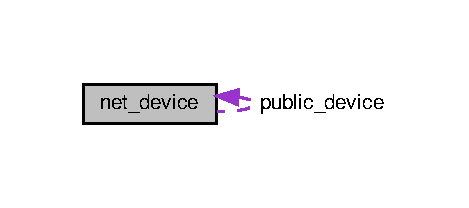
\includegraphics[width=225pt]{structnet__device__coll__graph}
\end{center}
\end{figure}
\subsection*{Public Attributes}
\begin{DoxyCompactItemize}
\item 
gboolean \hyperlink{structnet__device_af10284ed56562f2cd96fdb5ef22005d7}{is\+\_\+set}
\begin{DoxyCompactList}\small\item\em if the struct is set the has value T\+R\+UE \end{DoxyCompactList}\item 
uint32\+\_\+t \hyperlink{structnet__device_a8201165f1f516678fdbddffe8c786dd7}{dev\+\_\+pos}
\begin{DoxyCompactList}\small\item\em the depth of device in the local routing tree \end{DoxyCompactList}\item 
char \hyperlink{structnet__device_a683f88ff26dc8478bba51b95c39d9b92}{dev\+\_\+name} \mbox{[}16\mbox{]}
\begin{DoxyCompactList}\small\item\em the device name \end{DoxyCompactList}\item 
char \hyperlink{structnet__device_a65788d250a2b47bbbafeedfaa99ac695}{dev\+\_\+type} \mbox{[}20\mbox{]}
\begin{DoxyCompactList}\small\item\em the type device (physical and virtual) \end{DoxyCompactList}\item 
char \hyperlink{structnet__device_af33238d65f52774902101ad3255372f4}{dev\+\_\+method} \mbox{[}30\mbox{]}
\begin{DoxyCompactList}\small\item\em the method device uses (e.\+g. wifi) \end{DoxyCompactList}\item 
char \hyperlink{structnet__device_a92b5a35950b5bfaeb721be117e241528}{dev\+\_\+ip4} \mbox{[}16\mbox{]}
\begin{DoxyCompactList}\small\item\em the device I\+P\+V4 \end{DoxyCompactList}\item 
char \hyperlink{structnet__device_a7a8e6311682a530bfdeda88cfa808ed1}{dev\+\_\+ip6} \mbox{[}40\mbox{]}
\begin{DoxyCompactList}\small\item\em the device I\+P\+V6 \end{DoxyCompactList}\item 
char \hyperlink{structnet__device_ad708824b9b388d466795dc764d6fc477}{dev\+\_\+gateway} \mbox{[}40\mbox{]}
\begin{DoxyCompactList}\small\item\em the gateway device uses \end{DoxyCompactList}\item 
char \hyperlink{structnet__device_ac9ae8e657fb43f5baafd0fafcee819fa}{dev\+\_\+dns} \mbox{[}40\mbox{]}
\begin{DoxyCompactList}\small\item\em the dns device uses \end{DoxyCompactList}\item 
char \hyperlink{structnet__device_a1759ef9f942f991bff24268b2fc90c59}{dev\+\_\+active} \mbox{[}10\mbox{]}
\begin{DoxyCompactList}\small\item\em the status of device (A\+C\+T\+I\+VE and N\+O\+A\+C\+T\+I\+VE) \end{DoxyCompactList}\item 
char \hyperlink{structnet__device_a5f2de2bdeda68898f48a0d9347239e04}{dev\+\_\+wifi\+\_\+ap} \mbox{[}I\+W\+\_\+\+E\+S\+S\+I\+D\+\_\+\+M\+A\+X\+\_\+\+S\+I\+ZE+1\mbox{]}
\begin{DoxyCompactList}\small\item\em the access point name for wifi networks \end{DoxyCompactList}\item 
size\+\_\+t \hyperlink{structnet__device_a793c401280eb3afa81db485466aa77f2}{phy\+\_\+index}
\begin{DoxyCompactList}\small\item\em the index in the static global physical interfaces list. It may indicates the associated interface of a T\+UN device. \end{DoxyCompactList}\item 
char \hyperlink{structnet__device_ab9c29f0a4280c9f26bfedd0d7fd39789}{dev\+\_\+vpn\+\_\+profile} \mbox{[}N\+A\+M\+E\+\_\+\+M\+AX\mbox{]}
\begin{DoxyCompactList}\small\item\em the vpn profile name if the device used for a V\+PN. \end{DoxyCompactList}\item 
struct \hyperlink{structnet__device}{net\+\_\+device} $\ast$ \hyperlink{structnet__device_aa50aa45beac692be04baf4faf9d063d4}{public\+\_\+device}
\begin{DoxyCompactList}\small\item\em the pointer to the public (remote) device. It has value if the device is a physical device and it has a connection to the internet \end{DoxyCompactList}\item 
json\+\_\+object $\ast$ \hyperlink{structnet__device_ae3906a433b76b87e2c54069df9d5a342}{jobj}
\begin{DoxyCompactList}\small\item\em the J\+S\+ON representation of this device \end{DoxyCompactList}\end{DoxyCompactItemize}


\subsection{Detailed Description}
the struct stores the required information of network device in routes 

\subsection{Member Data Documentation}
\mbox{\Hypertarget{structnet__device_a1759ef9f942f991bff24268b2fc90c59}\label{structnet__device_a1759ef9f942f991bff24268b2fc90c59}} 
\index{net\+\_\+device@{net\+\_\+device}!dev\+\_\+active@{dev\+\_\+active}}
\index{dev\+\_\+active@{dev\+\_\+active}!net\+\_\+device@{net\+\_\+device}}
\subsubsection{\texorpdfstring{dev\+\_\+active}{dev\_active}}
{\footnotesize\ttfamily char net\+\_\+device\+::dev\+\_\+active\mbox{[}10\mbox{]}}



the status of device (A\+C\+T\+I\+VE and N\+O\+A\+C\+T\+I\+VE) 

\mbox{\Hypertarget{structnet__device_ac9ae8e657fb43f5baafd0fafcee819fa}\label{structnet__device_ac9ae8e657fb43f5baafd0fafcee819fa}} 
\index{net\+\_\+device@{net\+\_\+device}!dev\+\_\+dns@{dev\+\_\+dns}}
\index{dev\+\_\+dns@{dev\+\_\+dns}!net\+\_\+device@{net\+\_\+device}}
\subsubsection{\texorpdfstring{dev\+\_\+dns}{dev\_dns}}
{\footnotesize\ttfamily char net\+\_\+device\+::dev\+\_\+dns\mbox{[}40\mbox{]}}



the dns device uses 

\begin{DoxyNote}{Note}
may contain I\+P\+V6 
\end{DoxyNote}
\mbox{\Hypertarget{structnet__device_ad708824b9b388d466795dc764d6fc477}\label{structnet__device_ad708824b9b388d466795dc764d6fc477}} 
\index{net\+\_\+device@{net\+\_\+device}!dev\+\_\+gateway@{dev\+\_\+gateway}}
\index{dev\+\_\+gateway@{dev\+\_\+gateway}!net\+\_\+device@{net\+\_\+device}}
\subsubsection{\texorpdfstring{dev\+\_\+gateway}{dev\_gateway}}
{\footnotesize\ttfamily char net\+\_\+device\+::dev\+\_\+gateway\mbox{[}40\mbox{]}}



the gateway device uses 

\begin{DoxyNote}{Note}
may contain I\+P\+V6 
\end{DoxyNote}
\mbox{\Hypertarget{structnet__device_a92b5a35950b5bfaeb721be117e241528}\label{structnet__device_a92b5a35950b5bfaeb721be117e241528}} 
\index{net\+\_\+device@{net\+\_\+device}!dev\+\_\+ip4@{dev\+\_\+ip4}}
\index{dev\+\_\+ip4@{dev\+\_\+ip4}!net\+\_\+device@{net\+\_\+device}}
\subsubsection{\texorpdfstring{dev\+\_\+ip4}{dev\_ip4}}
{\footnotesize\ttfamily char net\+\_\+device\+::dev\+\_\+ip4\mbox{[}16\mbox{]}}



the device I\+P\+V4 

\mbox{\Hypertarget{structnet__device_a7a8e6311682a530bfdeda88cfa808ed1}\label{structnet__device_a7a8e6311682a530bfdeda88cfa808ed1}} 
\index{net\+\_\+device@{net\+\_\+device}!dev\+\_\+ip6@{dev\+\_\+ip6}}
\index{dev\+\_\+ip6@{dev\+\_\+ip6}!net\+\_\+device@{net\+\_\+device}}
\subsubsection{\texorpdfstring{dev\+\_\+ip6}{dev\_ip6}}
{\footnotesize\ttfamily char net\+\_\+device\+::dev\+\_\+ip6\mbox{[}40\mbox{]}}



the device I\+P\+V6 

\mbox{\Hypertarget{structnet__device_af33238d65f52774902101ad3255372f4}\label{structnet__device_af33238d65f52774902101ad3255372f4}} 
\index{net\+\_\+device@{net\+\_\+device}!dev\+\_\+method@{dev\+\_\+method}}
\index{dev\+\_\+method@{dev\+\_\+method}!net\+\_\+device@{net\+\_\+device}}
\subsubsection{\texorpdfstring{dev\+\_\+method}{dev\_method}}
{\footnotesize\ttfamily char net\+\_\+device\+::dev\+\_\+method\mbox{[}30\mbox{]}}



the method device uses (e.\+g. wifi) 

\mbox{\Hypertarget{structnet__device_a683f88ff26dc8478bba51b95c39d9b92}\label{structnet__device_a683f88ff26dc8478bba51b95c39d9b92}} 
\index{net\+\_\+device@{net\+\_\+device}!dev\+\_\+name@{dev\+\_\+name}}
\index{dev\+\_\+name@{dev\+\_\+name}!net\+\_\+device@{net\+\_\+device}}
\subsubsection{\texorpdfstring{dev\+\_\+name}{dev\_name}}
{\footnotesize\ttfamily char net\+\_\+device\+::dev\+\_\+name\mbox{[}16\mbox{]}}



the device name 

\mbox{\Hypertarget{structnet__device_a8201165f1f516678fdbddffe8c786dd7}\label{structnet__device_a8201165f1f516678fdbddffe8c786dd7}} 
\index{net\+\_\+device@{net\+\_\+device}!dev\+\_\+pos@{dev\+\_\+pos}}
\index{dev\+\_\+pos@{dev\+\_\+pos}!net\+\_\+device@{net\+\_\+device}}
\subsubsection{\texorpdfstring{dev\+\_\+pos}{dev\_pos}}
{\footnotesize\ttfamily uint32\+\_\+t net\+\_\+device\+::dev\+\_\+pos}



the depth of device in the local routing tree 

\mbox{\Hypertarget{structnet__device_a65788d250a2b47bbbafeedfaa99ac695}\label{structnet__device_a65788d250a2b47bbbafeedfaa99ac695}} 
\index{net\+\_\+device@{net\+\_\+device}!dev\+\_\+type@{dev\+\_\+type}}
\index{dev\+\_\+type@{dev\+\_\+type}!net\+\_\+device@{net\+\_\+device}}
\subsubsection{\texorpdfstring{dev\+\_\+type}{dev\_type}}
{\footnotesize\ttfamily char net\+\_\+device\+::dev\+\_\+type\mbox{[}20\mbox{]}}



the type device (physical and virtual) 

\mbox{\Hypertarget{structnet__device_ab9c29f0a4280c9f26bfedd0d7fd39789}\label{structnet__device_ab9c29f0a4280c9f26bfedd0d7fd39789}} 
\index{net\+\_\+device@{net\+\_\+device}!dev\+\_\+vpn\+\_\+profile@{dev\+\_\+vpn\+\_\+profile}}
\index{dev\+\_\+vpn\+\_\+profile@{dev\+\_\+vpn\+\_\+profile}!net\+\_\+device@{net\+\_\+device}}
\subsubsection{\texorpdfstring{dev\+\_\+vpn\+\_\+profile}{dev\_vpn\_profile}}
{\footnotesize\ttfamily char net\+\_\+device\+::dev\+\_\+vpn\+\_\+profile\mbox{[}N\+A\+M\+E\+\_\+\+M\+AX\mbox{]}}



the vpn profile name if the device used for a V\+PN. 

\mbox{\Hypertarget{structnet__device_a5f2de2bdeda68898f48a0d9347239e04}\label{structnet__device_a5f2de2bdeda68898f48a0d9347239e04}} 
\index{net\+\_\+device@{net\+\_\+device}!dev\+\_\+wifi\+\_\+ap@{dev\+\_\+wifi\+\_\+ap}}
\index{dev\+\_\+wifi\+\_\+ap@{dev\+\_\+wifi\+\_\+ap}!net\+\_\+device@{net\+\_\+device}}
\subsubsection{\texorpdfstring{dev\+\_\+wifi\+\_\+ap}{dev\_wifi\_ap}}
{\footnotesize\ttfamily char net\+\_\+device\+::dev\+\_\+wifi\+\_\+ap\mbox{[}I\+W\+\_\+\+E\+S\+S\+I\+D\+\_\+\+M\+A\+X\+\_\+\+S\+I\+ZE+1\mbox{]}}



the access point name for wifi networks 

\mbox{\Hypertarget{structnet__device_af10284ed56562f2cd96fdb5ef22005d7}\label{structnet__device_af10284ed56562f2cd96fdb5ef22005d7}} 
\index{net\+\_\+device@{net\+\_\+device}!is\+\_\+set@{is\+\_\+set}}
\index{is\+\_\+set@{is\+\_\+set}!net\+\_\+device@{net\+\_\+device}}
\subsubsection{\texorpdfstring{is\+\_\+set}{is\_set}}
{\footnotesize\ttfamily gboolean net\+\_\+device\+::is\+\_\+set}



if the struct is set the has value T\+R\+UE 

\mbox{\Hypertarget{structnet__device_ae3906a433b76b87e2c54069df9d5a342}\label{structnet__device_ae3906a433b76b87e2c54069df9d5a342}} 
\index{net\+\_\+device@{net\+\_\+device}!jobj@{jobj}}
\index{jobj@{jobj}!net\+\_\+device@{net\+\_\+device}}
\subsubsection{\texorpdfstring{jobj}{jobj}}
{\footnotesize\ttfamily json\+\_\+object$\ast$ net\+\_\+device\+::jobj}



the J\+S\+ON representation of this device 

\mbox{\Hypertarget{structnet__device_a793c401280eb3afa81db485466aa77f2}\label{structnet__device_a793c401280eb3afa81db485466aa77f2}} 
\index{net\+\_\+device@{net\+\_\+device}!phy\+\_\+index@{phy\+\_\+index}}
\index{phy\+\_\+index@{phy\+\_\+index}!net\+\_\+device@{net\+\_\+device}}
\subsubsection{\texorpdfstring{phy\+\_\+index}{phy\_index}}
{\footnotesize\ttfamily size\+\_\+t net\+\_\+device\+::phy\+\_\+index}



the index in the static global physical interfaces list. It may indicates the associated interface of a T\+UN device. 

\mbox{\Hypertarget{structnet__device_aa50aa45beac692be04baf4faf9d063d4}\label{structnet__device_aa50aa45beac692be04baf4faf9d063d4}} 
\index{net\+\_\+device@{net\+\_\+device}!public\+\_\+device@{public\+\_\+device}}
\index{public\+\_\+device@{public\+\_\+device}!net\+\_\+device@{net\+\_\+device}}
\subsubsection{\texorpdfstring{public\+\_\+device}{public\_device}}
{\footnotesize\ttfamily struct \hyperlink{structnet__device}{net\+\_\+device}$\ast$ net\+\_\+device\+::public\+\_\+device}



the pointer to the public (remote) device. It has value if the device is a physical device and it has a connection to the internet 



The documentation for this struct was generated from the following file\+:\begin{DoxyCompactItemize}
\item 
/home/sina/pantherx/networkinspection/git/include/\hyperlink{gnode-object_8h}{gnode-\/object.\+h}\end{DoxyCompactItemize}

\hypertarget{structnode__params}{}\section{node\+\_\+params Struct Reference}
\label{structnode__params}\index{node\+\_\+params@{node\+\_\+params}}


puts together the information extracted from rtnl\+\_\+route entries  


\subsection*{Public Attributes}
\begin{DoxyCompactItemize}
\item 
G\+Node $\ast$$\ast$ \hyperlink{structnode__params_a86b07f6f7d575e6b84723fbe1540771f}{node}
\item 
int $\ast$ \hyperlink{structnode__params_a5a78aaca912a055ee5920a7b222b0fd1}{roots}
\item 
char \hyperlink{structnode__params_a21fbc3409f16b2cbf0e00b76c041081f}{buf} \mbox{[}16\mbox{]}
\item 
char \hyperlink{structnode__params_ad543877faaca7b728c222501f57fb5a3}{gateway\+\_\+ipv4} \mbox{[}16\mbox{]}
\end{DoxyCompactItemize}


\subsection{Detailed Description}
puts together the information extracted from rtnl\+\_\+route entries 

\subsection{Member Data Documentation}
\mbox{\Hypertarget{structnode__params_a21fbc3409f16b2cbf0e00b76c041081f}\label{structnode__params_a21fbc3409f16b2cbf0e00b76c041081f}} 
\index{node\+\_\+params@{node\+\_\+params}!buf@{buf}}
\index{buf@{buf}!node\+\_\+params@{node\+\_\+params}}
\subsubsection{\texorpdfstring{buf}{buf}}
{\footnotesize\ttfamily char node\+\_\+params\+::buf\mbox{[}16\mbox{]}}

\mbox{\Hypertarget{structnode__params_ad543877faaca7b728c222501f57fb5a3}\label{structnode__params_ad543877faaca7b728c222501f57fb5a3}} 
\index{node\+\_\+params@{node\+\_\+params}!gateway\+\_\+ipv4@{gateway\+\_\+ipv4}}
\index{gateway\+\_\+ipv4@{gateway\+\_\+ipv4}!node\+\_\+params@{node\+\_\+params}}
\subsubsection{\texorpdfstring{gateway\+\_\+ipv4}{gateway\_ipv4}}
{\footnotesize\ttfamily char node\+\_\+params\+::gateway\+\_\+ipv4\mbox{[}16\mbox{]}}

\mbox{\Hypertarget{structnode__params_a86b07f6f7d575e6b84723fbe1540771f}\label{structnode__params_a86b07f6f7d575e6b84723fbe1540771f}} 
\index{node\+\_\+params@{node\+\_\+params}!node@{node}}
\index{node@{node}!node\+\_\+params@{node\+\_\+params}}
\subsubsection{\texorpdfstring{node}{node}}
{\footnotesize\ttfamily G\+Node$\ast$$\ast$ node\+\_\+params\+::node}

\mbox{\Hypertarget{structnode__params_a5a78aaca912a055ee5920a7b222b0fd1}\label{structnode__params_a5a78aaca912a055ee5920a7b222b0fd1}} 
\index{node\+\_\+params@{node\+\_\+params}!roots@{roots}}
\index{roots@{roots}!node\+\_\+params@{node\+\_\+params}}
\subsubsection{\texorpdfstring{roots}{roots}}
{\footnotesize\ttfamily int$\ast$ node\+\_\+params\+::roots}



The documentation for this struct was generated from the following file\+:\begin{DoxyCompactItemize}
\item 
/home/sina/pantherx/networkinspection/git/\hyperlink{route-tree_8c}{route-\/tree.\+c}\end{DoxyCompactItemize}

\hypertarget{structnode__search}{}\section{node\+\_\+search Struct Reference}
\label{structnode__search}\index{node\+\_\+search@{node\+\_\+search}}
\subsection*{Public Attributes}
\begin{DoxyCompactItemize}
\item 
char $\ast$ \hyperlink{structnode__search_ac34f755e54e8377475e42e4d9b1166cd}{ifa\+\_\+name}
\item 
G\+Node $\ast$ \hyperlink{structnode__search_acef2809bd08e8676c77b64dbb9f933d1}{krt\+\_\+node}
\end{DoxyCompactItemize}


\subsection{Member Data Documentation}
\mbox{\Hypertarget{structnode__search_ac34f755e54e8377475e42e4d9b1166cd}\label{structnode__search_ac34f755e54e8377475e42e4d9b1166cd}} 
\index{node\+\_\+search@{node\+\_\+search}!ifa\+\_\+name@{ifa\+\_\+name}}
\index{ifa\+\_\+name@{ifa\+\_\+name}!node\+\_\+search@{node\+\_\+search}}
\subsubsection{\texorpdfstring{ifa\+\_\+name}{ifa\_name}}
{\footnotesize\ttfamily char$\ast$ node\+\_\+search\+::ifa\+\_\+name}

\mbox{\Hypertarget{structnode__search_acef2809bd08e8676c77b64dbb9f933d1}\label{structnode__search_acef2809bd08e8676c77b64dbb9f933d1}} 
\index{node\+\_\+search@{node\+\_\+search}!krt\+\_\+node@{krt\+\_\+node}}
\index{krt\+\_\+node@{krt\+\_\+node}!node\+\_\+search@{node\+\_\+search}}
\subsubsection{\texorpdfstring{krt\+\_\+node}{krt\_node}}
{\footnotesize\ttfamily G\+Node$\ast$ node\+\_\+search\+::krt\+\_\+node}



The documentation for this struct was generated from the following file\+:\begin{DoxyCompactItemize}
\item 
/home/sina/pantherx/networkinspection/git/\hyperlink{route-tree_8c}{route-\/tree.\+c}\end{DoxyCompactItemize}

\hypertarget{structroute__node}{}\section{route\+\_\+node Struct Reference}
\label{structroute__node}\index{route\+\_\+node@{route\+\_\+node}}


the extracted information of a node in a kernel route table  




{\ttfamily \#include $<$route-\/tree.\+h$>$}

\subsection*{Public Attributes}
\begin{DoxyCompactItemize}
\item 
char \hyperlink{structroute__node_a4be6a66a552d88f360585c636ee70680}{if\+\_\+name} \mbox{[}I\+F\+N\+A\+M\+S\+IZ\mbox{]}
\item 
char \hyperlink{structroute__node_a27a750349a740654f57ad08fe87ff83f}{dst\+\_\+ipv4} \mbox{[}16\mbox{]}
\item 
char \hyperlink{structroute__node_a17ee301a4563560e6b7262dff9c8c0b8}{gateway\+\_\+ipv4} \mbox{[}16\mbox{]}
\item 
int \hyperlink{structroute__node_a43cbb1b4e49fd4a12395fa28a9febecc}{priority}
\end{DoxyCompactItemize}


\subsection{Detailed Description}
the extracted information of a node in a kernel route table 

\subsection{Member Data Documentation}
\mbox{\Hypertarget{structroute__node_a27a750349a740654f57ad08fe87ff83f}\label{structroute__node_a27a750349a740654f57ad08fe87ff83f}} 
\index{route\+\_\+node@{route\+\_\+node}!dst\+\_\+ipv4@{dst\+\_\+ipv4}}
\index{dst\+\_\+ipv4@{dst\+\_\+ipv4}!route\+\_\+node@{route\+\_\+node}}
\subsubsection{\texorpdfstring{dst\+\_\+ipv4}{dst\_ipv4}}
{\footnotesize\ttfamily char route\+\_\+node\+::dst\+\_\+ipv4\mbox{[}16\mbox{]}}

\mbox{\Hypertarget{structroute__node_a17ee301a4563560e6b7262dff9c8c0b8}\label{structroute__node_a17ee301a4563560e6b7262dff9c8c0b8}} 
\index{route\+\_\+node@{route\+\_\+node}!gateway\+\_\+ipv4@{gateway\+\_\+ipv4}}
\index{gateway\+\_\+ipv4@{gateway\+\_\+ipv4}!route\+\_\+node@{route\+\_\+node}}
\subsubsection{\texorpdfstring{gateway\+\_\+ipv4}{gateway\_ipv4}}
{\footnotesize\ttfamily char route\+\_\+node\+::gateway\+\_\+ipv4\mbox{[}16\mbox{]}}

\mbox{\Hypertarget{structroute__node_a4be6a66a552d88f360585c636ee70680}\label{structroute__node_a4be6a66a552d88f360585c636ee70680}} 
\index{route\+\_\+node@{route\+\_\+node}!if\+\_\+name@{if\+\_\+name}}
\index{if\+\_\+name@{if\+\_\+name}!route\+\_\+node@{route\+\_\+node}}
\subsubsection{\texorpdfstring{if\+\_\+name}{if\_name}}
{\footnotesize\ttfamily char route\+\_\+node\+::if\+\_\+name\mbox{[}I\+F\+N\+A\+M\+S\+IZ\mbox{]}}

\mbox{\Hypertarget{structroute__node_a43cbb1b4e49fd4a12395fa28a9febecc}\label{structroute__node_a43cbb1b4e49fd4a12395fa28a9febecc}} 
\index{route\+\_\+node@{route\+\_\+node}!priority@{priority}}
\index{priority@{priority}!route\+\_\+node@{route\+\_\+node}}
\subsubsection{\texorpdfstring{priority}{priority}}
{\footnotesize\ttfamily int route\+\_\+node\+::priority}



The documentation for this struct was generated from the following file\+:\begin{DoxyCompactItemize}
\item 
/home/sina/pantherx/networkinspection/git/include/\hyperlink{route-tree_8h}{route-\/tree.\+h}\end{DoxyCompactItemize}

\hypertarget{structurl__data}{}\section{url\+\_\+data Struct Reference}
\label{structurl__data}\index{url\+\_\+data@{url\+\_\+data}}


{\ttfamily \#include $<$public-\/ip.\+h$>$}

\subsection*{Public Attributes}
\begin{DoxyCompactItemize}
\item 
size\+\_\+t \hyperlink{structurl__data_a580f76d1bdde5b56bb7454e89a0d1ba8}{size}
\item 
char $\ast$ \hyperlink{structurl__data_ad3a5fe9c035fd8d6821363df1ce77725}{data}
\end{DoxyCompactItemize}


\subsection{Member Data Documentation}
\mbox{\Hypertarget{structurl__data_ad3a5fe9c035fd8d6821363df1ce77725}\label{structurl__data_ad3a5fe9c035fd8d6821363df1ce77725}} 
\index{url\+\_\+data@{url\+\_\+data}!data@{data}}
\index{data@{data}!url\+\_\+data@{url\+\_\+data}}
\subsubsection{\texorpdfstring{data}{data}}
{\footnotesize\ttfamily char$\ast$ url\+\_\+data\+::data}

\mbox{\Hypertarget{structurl__data_a580f76d1bdde5b56bb7454e89a0d1ba8}\label{structurl__data_a580f76d1bdde5b56bb7454e89a0d1ba8}} 
\index{url\+\_\+data@{url\+\_\+data}!size@{size}}
\index{size@{size}!url\+\_\+data@{url\+\_\+data}}
\subsubsection{\texorpdfstring{size}{size}}
{\footnotesize\ttfamily size\+\_\+t url\+\_\+data\+::size}



The documentation for this struct was generated from the following file\+:\begin{DoxyCompactItemize}
\item 
/home/sina/pantherx/networkinspection/git/include/\hyperlink{public-ip_8h}{public-\/ip.\+h}\end{DoxyCompactItemize}

\hypertarget{structvpnmethod}{}\section{vpnmethod Struct Reference}
\label{structvpnmethod}\index{vpnmethod@{vpnmethod}}


the struct to be put both V\+PN method and name together  




{\ttfamily \#include $<$route-\/tree.\+h$>$}

\subsection*{Public Attributes}
\begin{DoxyCompactItemize}
\item 
enum \hyperlink{route-tree_8h_a5b876670828c4e38106ba1c6d91024b7}{V\+P\+N\+\_\+\+M\+E\+T\+H\+O\+DS} \hyperlink{structvpnmethod_a33fa9abeccb46523aba83364fc44990f}{vpn\+\_\+method}
\item 
char \hyperlink{structvpnmethod_ac221598ca4c95900ae5b9fa404cbdb4d}{vpn\+\_\+name} \mbox{[}\hyperlink{route-tree_8h_a77ed9a5f9670b7a2d69c376d1199eddf}{M\+A\+X\+\_\+\+V\+P\+N\+\_\+\+N\+A\+ME}\mbox{]}
\end{DoxyCompactItemize}


\subsection{Detailed Description}
the struct to be put both V\+PN method and name together 

\subsection{Member Data Documentation}
\mbox{\Hypertarget{structvpnmethod_a33fa9abeccb46523aba83364fc44990f}\label{structvpnmethod_a33fa9abeccb46523aba83364fc44990f}} 
\index{vpnmethod@{vpnmethod}!vpn\+\_\+method@{vpn\+\_\+method}}
\index{vpn\+\_\+method@{vpn\+\_\+method}!vpnmethod@{vpnmethod}}
\subsubsection{\texorpdfstring{vpn\+\_\+method}{vpn\_method}}
{\footnotesize\ttfamily enum \hyperlink{route-tree_8h_a5b876670828c4e38106ba1c6d91024b7}{V\+P\+N\+\_\+\+M\+E\+T\+H\+O\+DS} vpnmethod\+::vpn\+\_\+method}

\mbox{\Hypertarget{structvpnmethod_ac221598ca4c95900ae5b9fa404cbdb4d}\label{structvpnmethod_ac221598ca4c95900ae5b9fa404cbdb4d}} 
\index{vpnmethod@{vpnmethod}!vpn\+\_\+name@{vpn\+\_\+name}}
\index{vpn\+\_\+name@{vpn\+\_\+name}!vpnmethod@{vpnmethod}}
\subsubsection{\texorpdfstring{vpn\+\_\+name}{vpn\_name}}
{\footnotesize\ttfamily char vpnmethod\+::vpn\+\_\+name\mbox{[}\hyperlink{route-tree_8h_a77ed9a5f9670b7a2d69c376d1199eddf}{M\+A\+X\+\_\+\+V\+P\+N\+\_\+\+N\+A\+ME}\mbox{]}}



The documentation for this struct was generated from the following file\+:\begin{DoxyCompactItemize}
\item 
/home/sina/pantherx/networkinspection/git/include/\hyperlink{route-tree_8h}{route-\/tree.\+h}\end{DoxyCompactItemize}

\chapter{File Documentation}
\hypertarget{app-profile_8c}{}\section{/home/sina/pantherx/networkinspection/git/app-\/profile.c File Reference}
\label{app-profile_8c}\index{/home/sina/pantherx/networkinspection/git/app-\/profile.\+c@{/home/sina/pantherx/networkinspection/git/app-\/profile.\+c}}
{\ttfamily \#include $<$app-\/profile.\+h$>$}\newline
{\ttfamily \#include $<$dirent.\+h$>$}\newline
{\ttfamily \#include $<$string.\+h$>$}\newline
{\ttfamily \#include $<$stdio.\+h$>$}\newline
{\ttfamily \#include $<$stdlib.\+h$>$}\newline
{\ttfamily \#include $<$libgen.\+h$>$}\newline
Include dependency graph for app-\/profile.c\+:\nopagebreak
\begin{figure}[H]
\begin{center}
\leavevmode
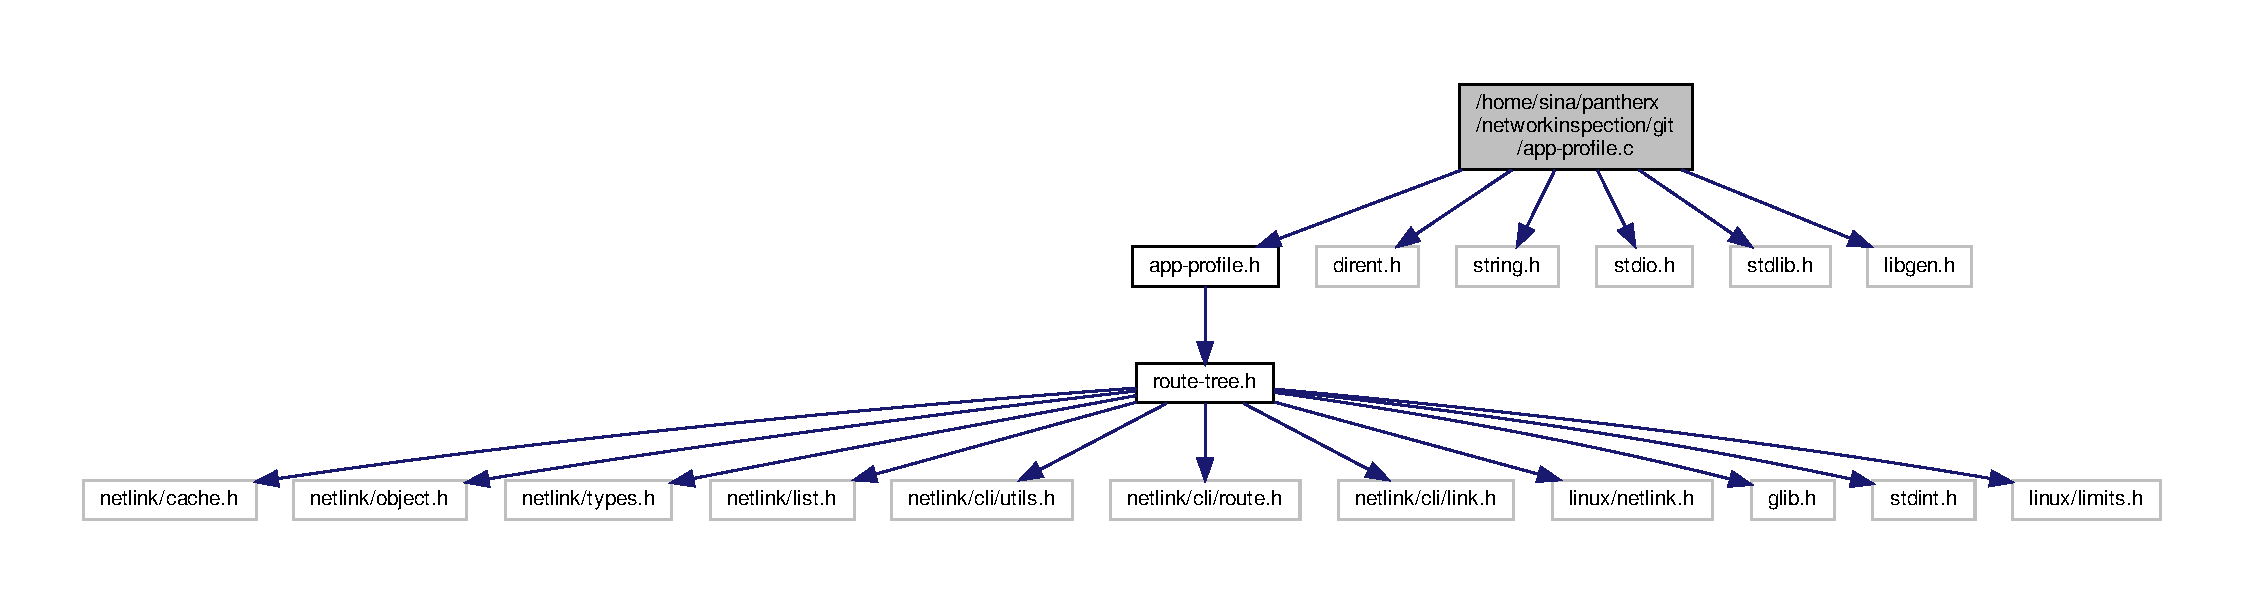
\includegraphics[width=350pt]{app-profile_8c__incl}
\end{center}
\end{figure}
\subsection*{Functions}
\begin{DoxyCompactItemize}
\item 
char $\ast$ \hyperlink{app-profile_8c_a59c7e3da3c5b7ecf10df2a5ef34b6953}{remove\+\_\+ext} (char $\ast$mystr)
\item 
int \hyperlink{app-profile_8c_a7ab4018359451259c67e57c83f9b7062}{get\+\_\+openvpn\+\_\+profile\+\_\+name} (char profile\+\_\+name\mbox{[}M\+A\+X\+\_\+\+V\+P\+N\+\_\+\+P\+R\+O\+F\+I\+L\+E\+\_\+\+N\+A\+ME\mbox{]})
\item 
int \hyperlink{app-profile_8c_aa32bea11cb1c8f99a45bc62cc8f5e455}{get\+\_\+vpn\+\_\+profile\+\_\+name} (enum V\+P\+N\+\_\+\+M\+E\+T\+H\+O\+DS vpn\+\_\+method, char profile\+\_\+name\mbox{[}M\+A\+X\+\_\+\+V\+P\+N\+\_\+\+P\+R\+O\+F\+I\+L\+E\+\_\+\+N\+A\+ME\mbox{]})
\end{DoxyCompactItemize}


\subsection{Function Documentation}
\mbox{\Hypertarget{app-profile_8c_a7ab4018359451259c67e57c83f9b7062}\label{app-profile_8c_a7ab4018359451259c67e57c83f9b7062}} 
\index{app-\/profile.\+c@{app-\/profile.\+c}!get\+\_\+openvpn\+\_\+profile\+\_\+name@{get\+\_\+openvpn\+\_\+profile\+\_\+name}}
\index{get\+\_\+openvpn\+\_\+profile\+\_\+name@{get\+\_\+openvpn\+\_\+profile\+\_\+name}!app-\/profile.\+c@{app-\/profile.\+c}}
\subsubsection{\texorpdfstring{get\+\_\+openvpn\+\_\+profile\+\_\+name()}{get\_openvpn\_profile\_name()}}
{\footnotesize\ttfamily int get\+\_\+openvpn\+\_\+profile\+\_\+name (\begin{DoxyParamCaption}\item[{char}]{profile\+\_\+name\mbox{[}\+M\+A\+X\+\_\+\+V\+P\+N\+\_\+\+P\+R\+O\+F\+I\+L\+E\+\_\+\+N\+A\+M\+E\mbox{]} }\end{DoxyParamCaption})}

\mbox{\Hypertarget{app-profile_8c_aa32bea11cb1c8f99a45bc62cc8f5e455}\label{app-profile_8c_aa32bea11cb1c8f99a45bc62cc8f5e455}} 
\index{app-\/profile.\+c@{app-\/profile.\+c}!get\+\_\+vpn\+\_\+profile\+\_\+name@{get\+\_\+vpn\+\_\+profile\+\_\+name}}
\index{get\+\_\+vpn\+\_\+profile\+\_\+name@{get\+\_\+vpn\+\_\+profile\+\_\+name}!app-\/profile.\+c@{app-\/profile.\+c}}
\subsubsection{\texorpdfstring{get\+\_\+vpn\+\_\+profile\+\_\+name()}{get\_vpn\_profile\_name()}}
{\footnotesize\ttfamily int get\+\_\+vpn\+\_\+profile\+\_\+name (\begin{DoxyParamCaption}\item[{enum V\+P\+N\+\_\+\+M\+E\+T\+H\+O\+DS}]{vpn\+\_\+method,  }\item[{char}]{profile\+\_\+name\mbox{[}\+M\+A\+X\+\_\+\+V\+P\+N\+\_\+\+P\+R\+O\+F\+I\+L\+E\+\_\+\+N\+A\+M\+E\mbox{]} }\end{DoxyParamCaption})}

\mbox{\Hypertarget{app-profile_8c_a59c7e3da3c5b7ecf10df2a5ef34b6953}\label{app-profile_8c_a59c7e3da3c5b7ecf10df2a5ef34b6953}} 
\index{app-\/profile.\+c@{app-\/profile.\+c}!remove\+\_\+ext@{remove\+\_\+ext}}
\index{remove\+\_\+ext@{remove\+\_\+ext}!app-\/profile.\+c@{app-\/profile.\+c}}
\subsubsection{\texorpdfstring{remove\+\_\+ext()}{remove\_ext()}}
{\footnotesize\ttfamily char$\ast$ remove\+\_\+ext (\begin{DoxyParamCaption}\item[{char $\ast$}]{mystr }\end{DoxyParamCaption})}


\hypertarget{checkroute_8c}{}\section{/home/sina/pantherx/networkinspection/git/checkroute.c File Reference}
\label{checkroute_8c}\index{/home/sina/pantherx/networkinspection/git/checkroute.\+c@{/home/sina/pantherx/networkinspection/git/checkroute.\+c}}
{\ttfamily \#include $<$arpa/inet.\+h$>$}\newline
{\ttfamily \#include $<$sys/socket.\+h$>$}\newline
{\ttfamily \#include $<$netdb.\+h$>$}\newline
{\ttfamily \#include $<$ifaddrs.\+h$>$}\newline
{\ttfamily \#include $<$stdio.\+h$>$}\newline
{\ttfamily \#include $<$stdlib.\+h$>$}\newline
{\ttfamily \#include $<$unistd.\+h$>$}\newline
{\ttfamily \#include $<$linux/if\+\_\+link.\+h$>$}\newline
{\ttfamily \#include $<$netlink/netlink.\+h$>$}\newline
{\ttfamily \#include $<$netlink/route/link.\+h$>$}\newline
{\ttfamily \#include $<$string.\+h$>$}\newline
{\ttfamily \#include $<$sys/types.\+h$>$}\newline
{\ttfamily \#include $<$sys/ioctl.\+h$>$}\newline
{\ttfamily \#include $<$net/if.\+h$>$}\newline
{\ttfamily \#include $<$sys/fcntl.\+h$>$}\newline
{\ttfamily \#include $<$linux/sockios.\+h$>$}\newline
{\ttfamily \#include $<$linux/ethtool.\+h$>$}\newline
Include dependency graph for checkroute.\+c\+:\nopagebreak
\begin{figure}[H]
\begin{center}
\leavevmode
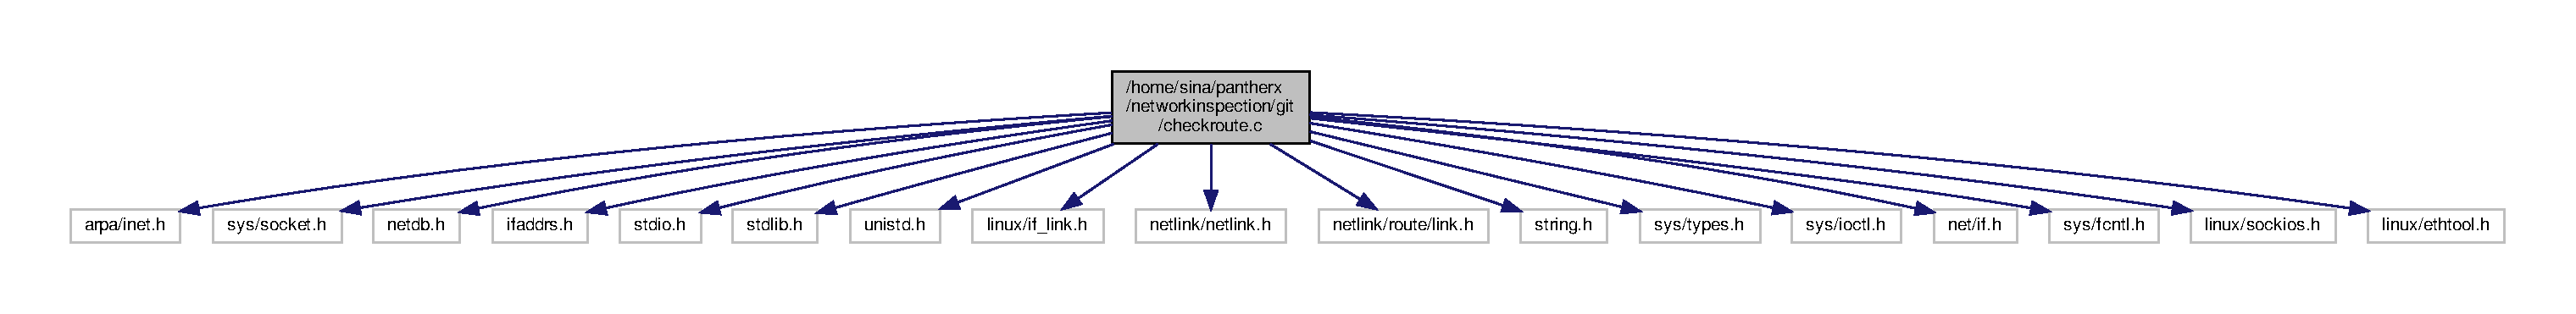
\includegraphics[width=350pt]{checkroute_8c__incl}
\end{center}
\end{figure}
\subsection*{Classes}
\begin{DoxyCompactItemize}
\item 
struct \hyperlink{structcmd__context}{cmd\+\_\+context}
\begin{DoxyCompactList}\small\item\em The struct represents the request message for ioctl system call. \end{DoxyCompactList}\end{DoxyCompactItemize}
\subsection*{Macros}
\begin{DoxyCompactItemize}
\item 
\#define \hyperlink{checkroute_8c_a369266c24eacffb87046522897a570d5}{\+\_\+\+G\+N\+U\+\_\+\+S\+O\+U\+R\+CE}~/$\ast$ To get defns of N\+I\+\_\+\+M\+A\+X\+S\+E\+RV and N\+I\+\_\+\+M\+A\+X\+H\+O\+ST $\ast$/
\end{DoxyCompactItemize}
\subsection*{Functions}
\begin{DoxyCompactItemize}
\item 
int \hyperlink{checkroute_8c_a6d58a8ebd8093edbe407365d8f3e93e5}{send\+\_\+ioctl} (struct \hyperlink{structcmd__context}{cmd\+\_\+context} $\ast$ctx, void $\ast$cmd)
\item 
int \hyperlink{checkroute_8c_a0ddf1224851353fc92bfbff6f499fa97}{main} (int argc, char $\ast$argv\mbox{[}$\,$\mbox{]})
\end{DoxyCompactItemize}


\subsection{Macro Definition Documentation}
\mbox{\Hypertarget{checkroute_8c_a369266c24eacffb87046522897a570d5}\label{checkroute_8c_a369266c24eacffb87046522897a570d5}} 
\index{checkroute.\+c@{checkroute.\+c}!\+\_\+\+G\+N\+U\+\_\+\+S\+O\+U\+R\+CE@{\+\_\+\+G\+N\+U\+\_\+\+S\+O\+U\+R\+CE}}
\index{\+\_\+\+G\+N\+U\+\_\+\+S\+O\+U\+R\+CE@{\+\_\+\+G\+N\+U\+\_\+\+S\+O\+U\+R\+CE}!checkroute.\+c@{checkroute.\+c}}
\subsubsection{\texorpdfstring{\+\_\+\+G\+N\+U\+\_\+\+S\+O\+U\+R\+CE}{\_GNU\_SOURCE}}
{\footnotesize\ttfamily \#define \+\_\+\+G\+N\+U\+\_\+\+S\+O\+U\+R\+CE~/$\ast$ To get defns of N\+I\+\_\+\+M\+A\+X\+S\+E\+RV and N\+I\+\_\+\+M\+A\+X\+H\+O\+ST $\ast$/}



\subsection{Function Documentation}
\mbox{\Hypertarget{checkroute_8c_a0ddf1224851353fc92bfbff6f499fa97}\label{checkroute_8c_a0ddf1224851353fc92bfbff6f499fa97}} 
\index{checkroute.\+c@{checkroute.\+c}!main@{main}}
\index{main@{main}!checkroute.\+c@{checkroute.\+c}}
\subsubsection{\texorpdfstring{main()}{main()}}
{\footnotesize\ttfamily int main (\begin{DoxyParamCaption}\item[{int}]{argc,  }\item[{char $\ast$}]{argv\mbox{[}$\,$\mbox{]} }\end{DoxyParamCaption})}

\mbox{\Hypertarget{checkroute_8c_a6d58a8ebd8093edbe407365d8f3e93e5}\label{checkroute_8c_a6d58a8ebd8093edbe407365d8f3e93e5}} 
\index{checkroute.\+c@{checkroute.\+c}!send\+\_\+ioctl@{send\+\_\+ioctl}}
\index{send\+\_\+ioctl@{send\+\_\+ioctl}!checkroute.\+c@{checkroute.\+c}}
\subsubsection{\texorpdfstring{send\+\_\+ioctl()}{send\_ioctl()}}
{\footnotesize\ttfamily int send\+\_\+ioctl (\begin{DoxyParamCaption}\item[{struct \hyperlink{structcmd__context}{cmd\+\_\+context} $\ast$}]{ctx,  }\item[{void $\ast$}]{cmd }\end{DoxyParamCaption})}


\hypertarget{ethtool-info_8c}{}\section{/home/sina/pantherx/networkinspection/git/ethtool-\/info.c File Reference}
\label{ethtool-info_8c}\index{/home/sina/pantherx/networkinspection/git/ethtool-\/info.\+c@{/home/sina/pantherx/networkinspection/git/ethtool-\/info.\+c}}
{\ttfamily \#include $<$ethtool-\/info.\+h$>$}\newline
{\ttfamily \#include $<$sys/socket.\+h$>$}\newline
{\ttfamily \#include $<$sys/fcntl.\+h$>$}\newline
{\ttfamily \#include $<$netinet/in.\+h$>$}\newline
{\ttfamily \#include $<$linux/sockios.\+h$>$}\newline
{\ttfamily \#include $<$linux/ethtool.\+h$>$}\newline
{\ttfamily \#include $<$stdio.\+h$>$}\newline
{\ttfamily \#include $<$stdlib.\+h$>$}\newline
Include dependency graph for ethtool-\/info.c\+:\nopagebreak
\begin{figure}[H]
\begin{center}
\leavevmode
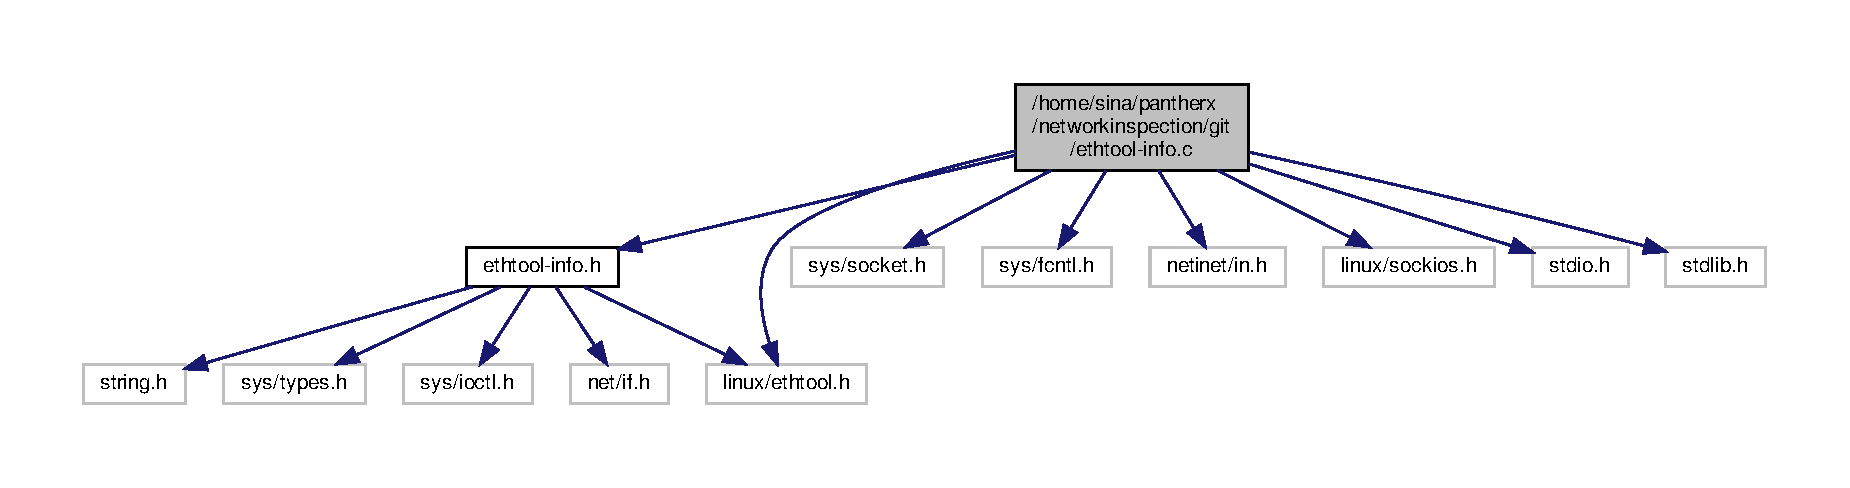
\includegraphics[width=350pt]{ethtool-info_8c__incl}
\end{center}
\end{figure}
\subsection*{Functions}
\begin{DoxyCompactItemize}
\item 
int \hyperlink{ethtool-info_8c_a6d58a8ebd8093edbe407365d8f3e93e5}{send\+\_\+ioctl} (struct \hyperlink{structcmd__context}{cmd\+\_\+context} $\ast$ctx, void $\ast$cmd)
\item 
int \hyperlink{ethtool-info_8c_a972c7feb6f25da37144ec7933d787147}{dump\+\_\+drvinfo} (struct ethtool\+\_\+drvinfo $\ast$info)
\item 
int \hyperlink{ethtool-info_8c_a92defcf2493dee90aeaac81e3b15572c}{do\+\_\+gdrv} (struct \hyperlink{structcmd__context}{cmd\+\_\+context} $\ast$ctx, struct ethtool\+\_\+drvinfo $\ast$drvinfo)
\item 
int \hyperlink{ethtool-info_8c_af4d8c485fa8cc199f6e1f27e949c9dc4}{get\+\_\+drv\+\_\+info} (char $\ast$ifa\+\_\+name, struct ethtool\+\_\+drvinfo $\ast$drvinfo)
\end{DoxyCompactItemize}


\subsection{Function Documentation}
\mbox{\Hypertarget{ethtool-info_8c_a92defcf2493dee90aeaac81e3b15572c}\label{ethtool-info_8c_a92defcf2493dee90aeaac81e3b15572c}} 
\index{ethtool-\/info.\+c@{ethtool-\/info.\+c}!do\+\_\+gdrv@{do\+\_\+gdrv}}
\index{do\+\_\+gdrv@{do\+\_\+gdrv}!ethtool-\/info.\+c@{ethtool-\/info.\+c}}
\subsubsection{\texorpdfstring{do\+\_\+gdrv()}{do\_gdrv()}}
{\footnotesize\ttfamily int do\+\_\+gdrv (\begin{DoxyParamCaption}\item[{struct \hyperlink{structcmd__context}{cmd\+\_\+context} $\ast$}]{ctx,  }\item[{struct ethtool\+\_\+drvinfo $\ast$}]{drvinfo }\end{DoxyParamCaption})}

\mbox{\Hypertarget{ethtool-info_8c_a972c7feb6f25da37144ec7933d787147}\label{ethtool-info_8c_a972c7feb6f25da37144ec7933d787147}} 
\index{ethtool-\/info.\+c@{ethtool-\/info.\+c}!dump\+\_\+drvinfo@{dump\+\_\+drvinfo}}
\index{dump\+\_\+drvinfo@{dump\+\_\+drvinfo}!ethtool-\/info.\+c@{ethtool-\/info.\+c}}
\subsubsection{\texorpdfstring{dump\+\_\+drvinfo()}{dump\_drvinfo()}}
{\footnotesize\ttfamily int dump\+\_\+drvinfo (\begin{DoxyParamCaption}\item[{struct ethtool\+\_\+drvinfo $\ast$}]{info }\end{DoxyParamCaption})}

\mbox{\Hypertarget{ethtool-info_8c_af4d8c485fa8cc199f6e1f27e949c9dc4}\label{ethtool-info_8c_af4d8c485fa8cc199f6e1f27e949c9dc4}} 
\index{ethtool-\/info.\+c@{ethtool-\/info.\+c}!get\+\_\+drv\+\_\+info@{get\+\_\+drv\+\_\+info}}
\index{get\+\_\+drv\+\_\+info@{get\+\_\+drv\+\_\+info}!ethtool-\/info.\+c@{ethtool-\/info.\+c}}
\subsubsection{\texorpdfstring{get\+\_\+drv\+\_\+info()}{get\_drv\_info()}}
{\footnotesize\ttfamily int get\+\_\+drv\+\_\+info (\begin{DoxyParamCaption}\item[{char $\ast$}]{ifa\+\_\+name,  }\item[{struct ethtool\+\_\+drvinfo $\ast$}]{drvinfo }\end{DoxyParamCaption})}

\mbox{\Hypertarget{ethtool-info_8c_a6d58a8ebd8093edbe407365d8f3e93e5}\label{ethtool-info_8c_a6d58a8ebd8093edbe407365d8f3e93e5}} 
\index{ethtool-\/info.\+c@{ethtool-\/info.\+c}!send\+\_\+ioctl@{send\+\_\+ioctl}}
\index{send\+\_\+ioctl@{send\+\_\+ioctl}!ethtool-\/info.\+c@{ethtool-\/info.\+c}}
\subsubsection{\texorpdfstring{send\+\_\+ioctl()}{send\_ioctl()}}
{\footnotesize\ttfamily int send\+\_\+ioctl (\begin{DoxyParamCaption}\item[{struct \hyperlink{structcmd__context}{cmd\+\_\+context} $\ast$}]{ctx,  }\item[{void $\ast$}]{cmd }\end{DoxyParamCaption})}


\hypertarget{gnode-object_8c}{}\section{/home/sina/pantherx/networkinspection/git/gnode-\/object.c File Reference}
\label{gnode-object_8c}\index{/home/sina/pantherx/networkinspection/git/gnode-\/object.\+c@{/home/sina/pantherx/networkinspection/git/gnode-\/object.\+c}}
{\ttfamily \#include $<$gnode-\/object.\+h$>$}\newline
{\ttfamily \#include $<$stdio.\+h$>$}\newline
Include dependency graph for gnode-\/object.c\+:\nopagebreak
\begin{figure}[H]
\begin{center}
\leavevmode
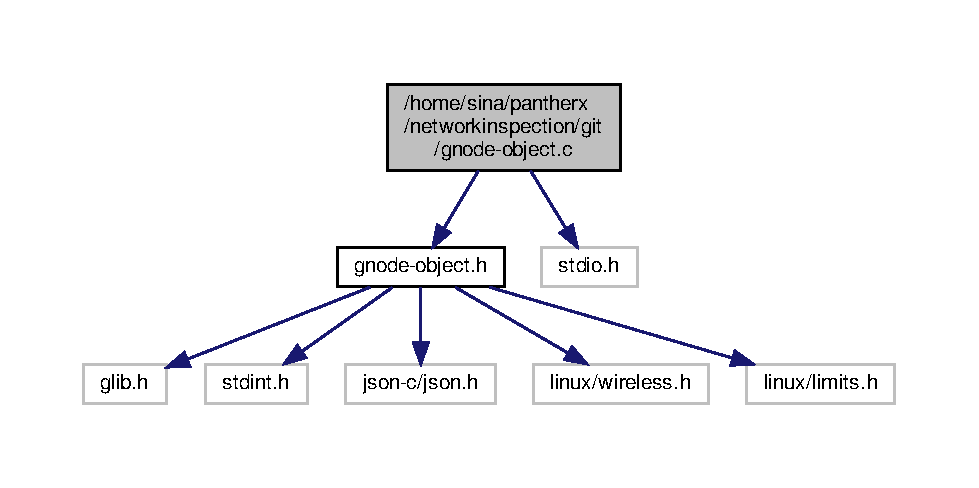
\includegraphics[width=224pt]{gnode-object_8c__incl}
\end{center}
\end{figure}
\subsection*{Functions}
\begin{DoxyCompactItemize}
\item 
Net\+Device $\ast$ \hyperlink{gnode-object_8c_ae666b3f20895e60917e691c81d464235}{net\+\_\+device\+\_\+new} ()
\item 
void \hyperlink{gnode-object_8c_af75477fcbe781bc0b17c75c1ad6d1606}{net\+\_\+device\+\_\+free} (Net\+Device $\ast$nd)
\item 
void \hyperlink{gnode-object_8c_a37bf3d0e5222ef4eeda3b40df60a1812}{internal\+\_\+traverse\+\_\+json\+\_\+func} (Net\+Device $\ast$device)
\item 
gboolean \hyperlink{gnode-object_8c_acde5d3e413f355d1b912f0dcb9d4cdc1}{traverse\+\_\+json\+\_\+func} (G\+Node $\ast$node, gpointer data)
\item 
gboolean \hyperlink{gnode-object_8c_a0d906716c0b2c59e34bff01153dc23d2}{traverse\+\_\+json\+\_\+array\+\_\+func} (G\+Node $\ast$node, gpointer data)
\end{DoxyCompactItemize}


\subsection{Function Documentation}
\mbox{\Hypertarget{gnode-object_8c_a37bf3d0e5222ef4eeda3b40df60a1812}\label{gnode-object_8c_a37bf3d0e5222ef4eeda3b40df60a1812}} 
\index{gnode-\/object.\+c@{gnode-\/object.\+c}!internal\+\_\+traverse\+\_\+json\+\_\+func@{internal\+\_\+traverse\+\_\+json\+\_\+func}}
\index{internal\+\_\+traverse\+\_\+json\+\_\+func@{internal\+\_\+traverse\+\_\+json\+\_\+func}!gnode-\/object.\+c@{gnode-\/object.\+c}}
\subsubsection{\texorpdfstring{internal\+\_\+traverse\+\_\+json\+\_\+func()}{internal\_traverse\_json\_func()}}
{\footnotesize\ttfamily void internal\+\_\+traverse\+\_\+json\+\_\+func (\begin{DoxyParamCaption}\item[{Net\+Device $\ast$}]{device }\end{DoxyParamCaption})}

\mbox{\Hypertarget{gnode-object_8c_af75477fcbe781bc0b17c75c1ad6d1606}\label{gnode-object_8c_af75477fcbe781bc0b17c75c1ad6d1606}} 
\index{gnode-\/object.\+c@{gnode-\/object.\+c}!net\+\_\+device\+\_\+free@{net\+\_\+device\+\_\+free}}
\index{net\+\_\+device\+\_\+free@{net\+\_\+device\+\_\+free}!gnode-\/object.\+c@{gnode-\/object.\+c}}
\subsubsection{\texorpdfstring{net\+\_\+device\+\_\+free()}{net\_device\_free()}}
{\footnotesize\ttfamily void net\+\_\+device\+\_\+free (\begin{DoxyParamCaption}\item[{Net\+Device $\ast$}]{nd }\end{DoxyParamCaption})}

\mbox{\Hypertarget{gnode-object_8c_ae666b3f20895e60917e691c81d464235}\label{gnode-object_8c_ae666b3f20895e60917e691c81d464235}} 
\index{gnode-\/object.\+c@{gnode-\/object.\+c}!net\+\_\+device\+\_\+new@{net\+\_\+device\+\_\+new}}
\index{net\+\_\+device\+\_\+new@{net\+\_\+device\+\_\+new}!gnode-\/object.\+c@{gnode-\/object.\+c}}
\subsubsection{\texorpdfstring{net\+\_\+device\+\_\+new()}{net\_device\_new()}}
{\footnotesize\ttfamily Net\+Device$\ast$ net\+\_\+device\+\_\+new (\begin{DoxyParamCaption}{ }\end{DoxyParamCaption})}

\mbox{\Hypertarget{gnode-object_8c_a0d906716c0b2c59e34bff01153dc23d2}\label{gnode-object_8c_a0d906716c0b2c59e34bff01153dc23d2}} 
\index{gnode-\/object.\+c@{gnode-\/object.\+c}!traverse\+\_\+json\+\_\+array\+\_\+func@{traverse\+\_\+json\+\_\+array\+\_\+func}}
\index{traverse\+\_\+json\+\_\+array\+\_\+func@{traverse\+\_\+json\+\_\+array\+\_\+func}!gnode-\/object.\+c@{gnode-\/object.\+c}}
\subsubsection{\texorpdfstring{traverse\+\_\+json\+\_\+array\+\_\+func()}{traverse\_json\_array\_func()}}
{\footnotesize\ttfamily gboolean traverse\+\_\+json\+\_\+array\+\_\+func (\begin{DoxyParamCaption}\item[{G\+Node $\ast$}]{node,  }\item[{gpointer}]{data }\end{DoxyParamCaption})}

\mbox{\Hypertarget{gnode-object_8c_acde5d3e413f355d1b912f0dcb9d4cdc1}\label{gnode-object_8c_acde5d3e413f355d1b912f0dcb9d4cdc1}} 
\index{gnode-\/object.\+c@{gnode-\/object.\+c}!traverse\+\_\+json\+\_\+func@{traverse\+\_\+json\+\_\+func}}
\index{traverse\+\_\+json\+\_\+func@{traverse\+\_\+json\+\_\+func}!gnode-\/object.\+c@{gnode-\/object.\+c}}
\subsubsection{\texorpdfstring{traverse\+\_\+json\+\_\+func()}{traverse\_json\_func()}}
{\footnotesize\ttfamily gboolean traverse\+\_\+json\+\_\+func (\begin{DoxyParamCaption}\item[{G\+Node $\ast$}]{node,  }\item[{gpointer}]{data }\end{DoxyParamCaption})}


\hypertarget{app-profile_8h}{}\section{/home/sina/pantherx/networkinspection/git/include/app-\/profile.h File Reference}
\label{app-profile_8h}\index{/home/sina/pantherx/networkinspection/git/include/app-\/profile.\+h@{/home/sina/pantherx/networkinspection/git/include/app-\/profile.\+h}}
{\ttfamily \#include $<$route-\/tree.\+h$>$}\newline
Include dependency graph for app-\/profile.h\+:\nopagebreak
\begin{figure}[H]
\begin{center}
\leavevmode
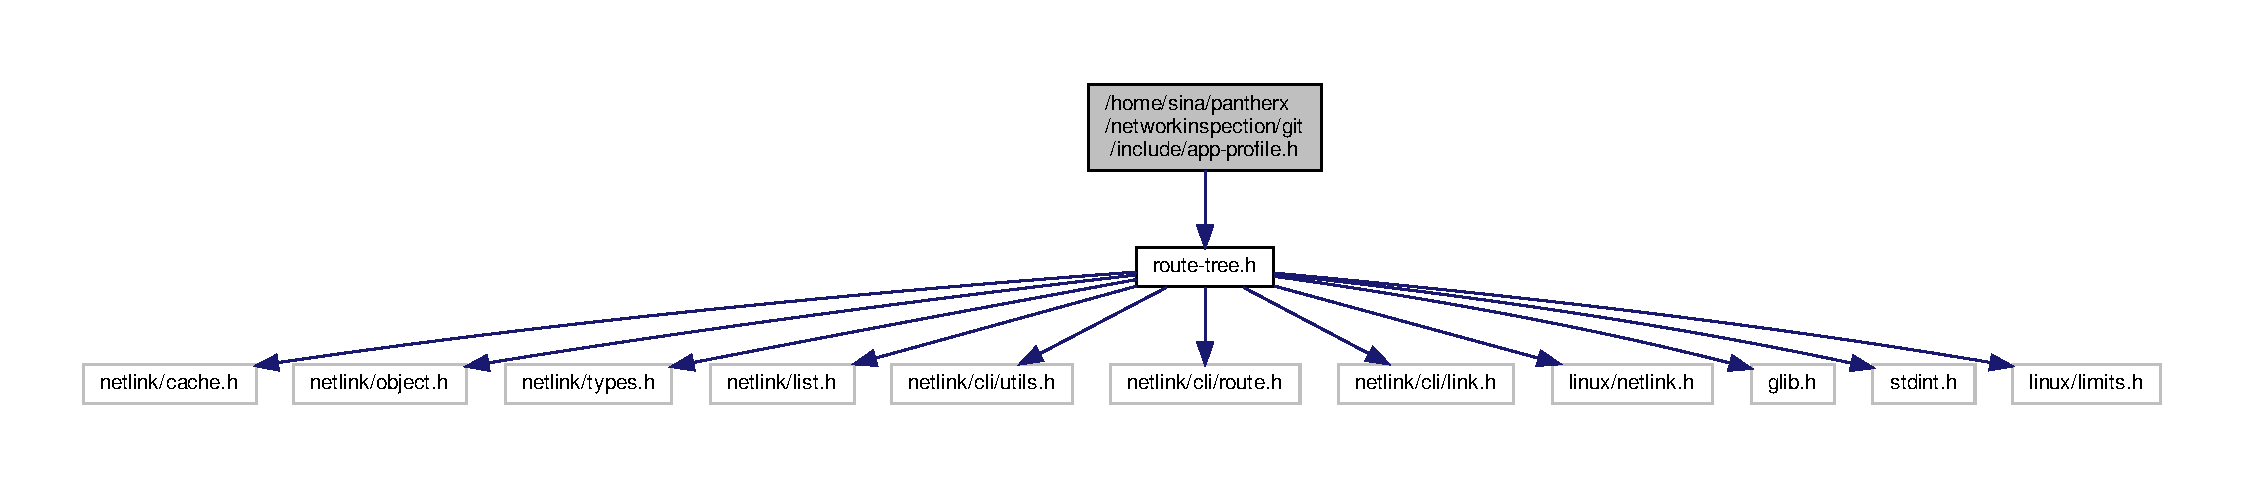
\includegraphics[width=350pt]{app-profile_8h__incl}
\end{center}
\end{figure}
This graph shows which files directly or indirectly include this file\+:\nopagebreak
\begin{figure}[H]
\begin{center}
\leavevmode
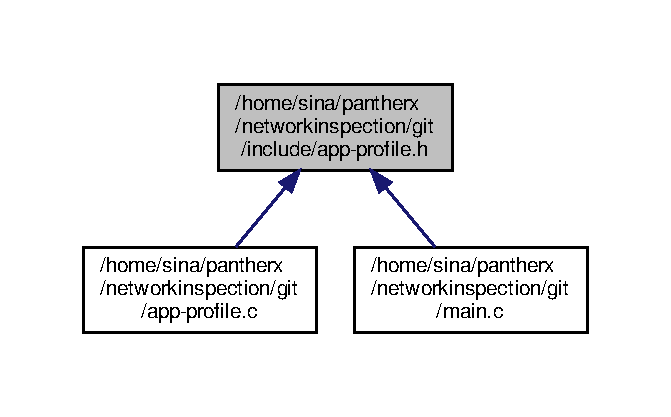
\includegraphics[width=322pt]{app-profile_8h__dep__incl}
\end{center}
\end{figure}
\subsection*{Functions}
\begin{DoxyCompactItemize}
\item 
int \hyperlink{app-profile_8h_a2af00bda795682f62e77417d4969e2e5}{get\+\_\+vpn\+\_\+profile\+\_\+name} (enum \hyperlink{route-tree_8h_a5b876670828c4e38106ba1c6d91024b7}{V\+P\+N\+\_\+\+M\+E\+T\+H\+O\+DS} vpn\+\_\+method, char profile\+\_\+name\mbox{[}\hyperlink{route-tree_8h_a77ed9a5f9670b7a2d69c376d1199eddf}{M\+A\+X\+\_\+\+V\+P\+N\+\_\+\+N\+A\+ME}\mbox{]})
\begin{DoxyCompactList}\small\item\em Finds the V\+PN\textquotesingle{}s profile name. \end{DoxyCompactList}\end{DoxyCompactItemize}


\subsection{Function Documentation}
\mbox{\Hypertarget{app-profile_8h_a2af00bda795682f62e77417d4969e2e5}\label{app-profile_8h_a2af00bda795682f62e77417d4969e2e5}} 
\index{app-\/profile.\+h@{app-\/profile.\+h}!get\+\_\+vpn\+\_\+profile\+\_\+name@{get\+\_\+vpn\+\_\+profile\+\_\+name}}
\index{get\+\_\+vpn\+\_\+profile\+\_\+name@{get\+\_\+vpn\+\_\+profile\+\_\+name}!app-\/profile.\+h@{app-\/profile.\+h}}
\subsubsection{\texorpdfstring{get\+\_\+vpn\+\_\+profile\+\_\+name()}{get\_vpn\_profile\_name()}}
{\footnotesize\ttfamily int get\+\_\+vpn\+\_\+profile\+\_\+name (\begin{DoxyParamCaption}\item[{enum \hyperlink{route-tree_8h_a5b876670828c4e38106ba1c6d91024b7}{V\+P\+N\+\_\+\+M\+E\+T\+H\+O\+DS}}]{vpn\+\_\+method,  }\item[{char}]{profile\+\_\+name\mbox{[}\+M\+A\+X\+\_\+\+V\+P\+N\+\_\+\+N\+A\+M\+E\mbox{]} }\end{DoxyParamCaption})}



Finds the V\+PN\textquotesingle{}s profile name. 

The function finds the profile name of the V\+PN if there is any.

\begin{DoxySeeAlso}{See also}
\href{https://wiki.pantherx.org}{\tt https\+://wiki.\+pantherx.\+org} 
\end{DoxySeeAlso}
\begin{DoxyRefDesc}{Todo}
\item[\hyperlink{todo__todo000008}{Todo}]T\+O\+DO Support tap-\/based interfaces.\end{DoxyRefDesc}



\begin{DoxyParams}[1]{Parameters}
\mbox{\tt in}  & {\em vpn\+\_\+method} & the method used for V\+PN i.\+e. O\+P\+E\+N\+V\+PN. \\
\hline
\mbox{\tt out}  & {\em profile\+\_\+name} & the found name of the profile if there is any. \\
\hline
\end{DoxyParams}
\begin{DoxyReturn}{Returns}
indicates that the profile\+\_\+name contains a valid name. The value -\/1 means unsupported V\+PN method. The value 0 means a default or no profile name. The value 1 means profile\+\_\+name contains a valid value. 
\end{DoxyReturn}
\begin{DoxyPrecond}{Precondition}
The vpn\+\_\+method must be retrieved first. 
\end{DoxyPrecond}

\hypertarget{arg-info_8h}{}\section{/home/sina/pantherx/networkinspection/git/include/arg-\/info.h File Reference}
\label{arg-info_8h}\index{/home/sina/pantherx/networkinspection/git/include/arg-\/info.\+h@{/home/sina/pantherx/networkinspection/git/include/arg-\/info.\+h}}
{\ttfamily \#include $<$argp.\+h$>$}\newline
{\ttfamily \#include $<$stdbool.\+h$>$}\newline
{\ttfamily \#include $<$string.\+h$>$}\newline
Include dependency graph for arg-\/info.h\+:\nopagebreak
\begin{figure}[H]
\begin{center}
\leavevmode
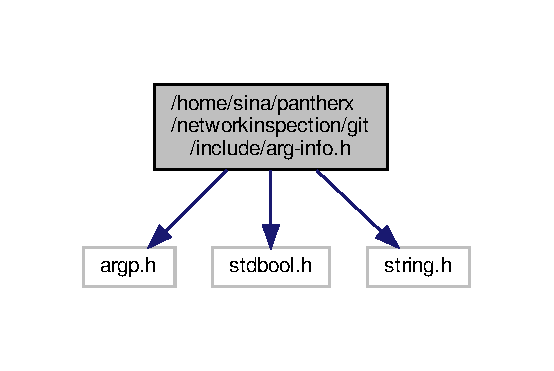
\includegraphics[width=266pt]{arg-info_8h__incl}
\end{center}
\end{figure}
This graph shows which files directly or indirectly include this file\+:\nopagebreak
\begin{figure}[H]
\begin{center}
\leavevmode
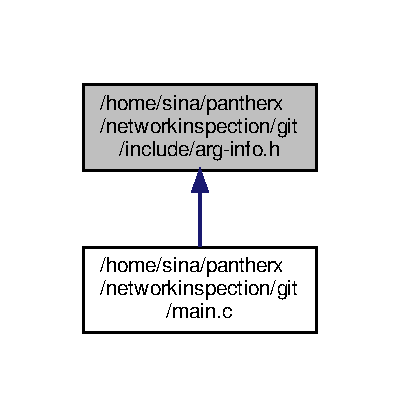
\includegraphics[width=192pt]{arg-info_8h__dep__incl}
\end{center}
\end{figure}
\subsection*{Classes}
\begin{DoxyCompactItemize}
\item 
struct \hyperlink{structarguments}{arguments}
\begin{DoxyCompactList}\small\item\em used by main to fetch the parsed arguments \end{DoxyCompactList}\end{DoxyCompactItemize}
\subsection*{Enumerations}
\begin{DoxyCompactItemize}
\item 
enum \hyperlink{arg-info_8h_ab4e88c89b3b7ea1735996cc4def22d58}{Format} \{ \hyperlink{arg-info_8h_ab4e88c89b3b7ea1735996cc4def22d58aa5210511e3859748f136ab50c313ef05}{J\+S\+ON}, 
\hyperlink{arg-info_8h_ab4e88c89b3b7ea1735996cc4def22d58afde1c37e079bb0efad8943458c4c6da8}{C\+XX}
 \}\begin{DoxyCompactList}\small\item\em the type of the output format \end{DoxyCompactList}
\end{DoxyCompactItemize}
\subsection*{Functions}
\begin{DoxyCompactItemize}
\item 
error\+\_\+t \hyperlink{arg-info_8h_a5fb6abc38ef248ec154591e0dd392c1b}{parse\+\_\+opt} (int key, char $\ast$arg, struct argp\+\_\+state $\ast$state)
\begin{DoxyCompactList}\small\item\em Parse a single option. \end{DoxyCompactList}\end{DoxyCompactItemize}
\subsection*{Variables}
\begin{DoxyCompactItemize}
\item 
const char $\ast$ \hyperlink{arg-info_8h_a62f73ea01c816f1996aed4c66f57c4fb}{argp\+\_\+program\+\_\+version} = \char`\"{}0.\+0.\+9\char`\"{}
\begin{DoxyCompactList}\small\item\em version of the px-\/network-\/inspection \end{DoxyCompactList}\item 
const char $\ast$ \hyperlink{arg-info_8h_aaa037e59f26a80a8a2e35e6f2364004d}{argp\+\_\+program\+\_\+bug\+\_\+address} = \char`\"{}$<$s.\+mahmood@pantherx.\+org$>$\char`\"{}
\begin{DoxyCompactList}\small\item\em the bug report email address. \end{DoxyCompactList}\item 
char \hyperlink{arg-info_8h_af6164deb8a824f8cb2b9147cfc3174f5}{doc} \mbox{[}$\,$\mbox{]} = \char`\"{}A utility to collect network routing details of local machine.\char`\"{}
\begin{DoxyCompactList}\small\item\em Program documentation. \end{DoxyCompactList}\item 
char \hyperlink{arg-info_8h_a91b08784b3668a8a1fbe2eec1947fb9d}{args\+\_\+doc} \mbox{[}$\,$\mbox{]} = \char`\"{}\char`\"{}
\begin{DoxyCompactList}\small\item\em A description of the arguments we accept. \end{DoxyCompactList}\item 
struct argp\+\_\+option \hyperlink{arg-info_8h_abc1fd3a47aea6a8944038c9100eb9135}{options} \mbox{[}$\,$\mbox{]}
\begin{DoxyCompactList}\small\item\em The options we understand. \end{DoxyCompactList}\item 
struct argp \hyperlink{arg-info_8h_ab70c96531b1b652d70c221cfaf3207f3}{argp} = \{ \hyperlink{arg-info_8h_abc1fd3a47aea6a8944038c9100eb9135}{options}, \hyperlink{arg-info_8h_a5fb6abc38ef248ec154591e0dd392c1b}{parse\+\_\+opt}, \hyperlink{arg-info_8h_a91b08784b3668a8a1fbe2eec1947fb9d}{args\+\_\+doc}, \hyperlink{arg-info_8h_af6164deb8a824f8cb2b9147cfc3174f5}{doc}\}
\begin{DoxyCompactList}\small\item\em The argp parser. \end{DoxyCompactList}\end{DoxyCompactItemize}


\subsection{Enumeration Type Documentation}
\mbox{\Hypertarget{arg-info_8h_ab4e88c89b3b7ea1735996cc4def22d58}\label{arg-info_8h_ab4e88c89b3b7ea1735996cc4def22d58}} 
\index{arg-\/info.\+h@{arg-\/info.\+h}!Format@{Format}}
\index{Format@{Format}!arg-\/info.\+h@{arg-\/info.\+h}}
\subsubsection{\texorpdfstring{Format}{Format}}
{\footnotesize\ttfamily enum \hyperlink{arg-info_8h_ab4e88c89b3b7ea1735996cc4def22d58}{Format}}



the type of the output format 

\begin{DoxyEnumFields}{Enumerator}
\raisebox{\heightof{T}}[0pt][0pt]{\index{J\+S\+ON@{J\+S\+ON}!arg-\/info.\+h@{arg-\/info.\+h}}\index{arg-\/info.\+h@{arg-\/info.\+h}!J\+S\+ON@{J\+S\+ON}}}\mbox{\Hypertarget{arg-info_8h_ab4e88c89b3b7ea1735996cc4def22d58aa5210511e3859748f136ab50c313ef05}\label{arg-info_8h_ab4e88c89b3b7ea1735996cc4def22d58aa5210511e3859748f136ab50c313ef05}} 
J\+S\+ON&\\
\hline

\raisebox{\heightof{T}}[0pt][0pt]{\index{C\+XX@{C\+XX}!arg-\/info.\+h@{arg-\/info.\+h}}\index{arg-\/info.\+h@{arg-\/info.\+h}!C\+XX@{C\+XX}}}\mbox{\Hypertarget{arg-info_8h_ab4e88c89b3b7ea1735996cc4def22d58afde1c37e079bb0efad8943458c4c6da8}\label{arg-info_8h_ab4e88c89b3b7ea1735996cc4def22d58afde1c37e079bb0efad8943458c4c6da8}} 
C\+XX&\\
\hline

\end{DoxyEnumFields}


\subsection{Function Documentation}
\mbox{\Hypertarget{arg-info_8h_a5fb6abc38ef248ec154591e0dd392c1b}\label{arg-info_8h_a5fb6abc38ef248ec154591e0dd392c1b}} 
\index{arg-\/info.\+h@{arg-\/info.\+h}!parse\+\_\+opt@{parse\+\_\+opt}}
\index{parse\+\_\+opt@{parse\+\_\+opt}!arg-\/info.\+h@{arg-\/info.\+h}}
\subsubsection{\texorpdfstring{parse\+\_\+opt()}{parse\_opt()}}
{\footnotesize\ttfamily error\+\_\+t parse\+\_\+opt (\begin{DoxyParamCaption}\item[{int}]{key,  }\item[{char $\ast$}]{arg,  }\item[{struct argp\+\_\+state $\ast$}]{state }\end{DoxyParamCaption})}



Parse a single option. 

The function is a call-\/back that is called by the arg-\/parser.

\begin{DoxySeeAlso}{See also}
\href{https://wiki.pantherx.org}{\tt https\+://wiki.\+pantherx.\+org}
\end{DoxySeeAlso}
\begin{DoxyNote}{Note}
not to call from code. 
\end{DoxyNote}
\begin{DoxyPostcond}{Postcondition}
use inf struct argp. 
\end{DoxyPostcond}


\subsection{Variable Documentation}
\mbox{\Hypertarget{arg-info_8h_ab70c96531b1b652d70c221cfaf3207f3}\label{arg-info_8h_ab70c96531b1b652d70c221cfaf3207f3}} 
\index{arg-\/info.\+h@{arg-\/info.\+h}!argp@{argp}}
\index{argp@{argp}!arg-\/info.\+h@{arg-\/info.\+h}}
\subsubsection{\texorpdfstring{argp}{argp}}
{\footnotesize\ttfamily struct argp argp = \{ \hyperlink{arg-info_8h_abc1fd3a47aea6a8944038c9100eb9135}{options}, \hyperlink{arg-info_8h_a5fb6abc38ef248ec154591e0dd392c1b}{parse\+\_\+opt}, \hyperlink{arg-info_8h_a91b08784b3668a8a1fbe2eec1947fb9d}{args\+\_\+doc}, \hyperlink{arg-info_8h_af6164deb8a824f8cb2b9147cfc3174f5}{doc}\}}



The argp parser. 

\mbox{\Hypertarget{arg-info_8h_aaa037e59f26a80a8a2e35e6f2364004d}\label{arg-info_8h_aaa037e59f26a80a8a2e35e6f2364004d}} 
\index{arg-\/info.\+h@{arg-\/info.\+h}!argp\+\_\+program\+\_\+bug\+\_\+address@{argp\+\_\+program\+\_\+bug\+\_\+address}}
\index{argp\+\_\+program\+\_\+bug\+\_\+address@{argp\+\_\+program\+\_\+bug\+\_\+address}!arg-\/info.\+h@{arg-\/info.\+h}}
\subsubsection{\texorpdfstring{argp\+\_\+program\+\_\+bug\+\_\+address}{argp\_program\_bug\_address}}
{\footnotesize\ttfamily const char$\ast$ argp\+\_\+program\+\_\+bug\+\_\+address = \char`\"{}$<$s.\+mahmood@pantherx.\+org$>$\char`\"{}}



the bug report email address. 

\mbox{\Hypertarget{arg-info_8h_a62f73ea01c816f1996aed4c66f57c4fb}\label{arg-info_8h_a62f73ea01c816f1996aed4c66f57c4fb}} 
\index{arg-\/info.\+h@{arg-\/info.\+h}!argp\+\_\+program\+\_\+version@{argp\+\_\+program\+\_\+version}}
\index{argp\+\_\+program\+\_\+version@{argp\+\_\+program\+\_\+version}!arg-\/info.\+h@{arg-\/info.\+h}}
\subsubsection{\texorpdfstring{argp\+\_\+program\+\_\+version}{argp\_program\_version}}
{\footnotesize\ttfamily const char$\ast$ argp\+\_\+program\+\_\+version = \char`\"{}0.\+0.\+9\char`\"{}}



version of the px-\/network-\/inspection 

\mbox{\Hypertarget{arg-info_8h_a91b08784b3668a8a1fbe2eec1947fb9d}\label{arg-info_8h_a91b08784b3668a8a1fbe2eec1947fb9d}} 
\index{arg-\/info.\+h@{arg-\/info.\+h}!args\+\_\+doc@{args\+\_\+doc}}
\index{args\+\_\+doc@{args\+\_\+doc}!arg-\/info.\+h@{arg-\/info.\+h}}
\subsubsection{\texorpdfstring{args\+\_\+doc}{args\_doc}}
{\footnotesize\ttfamily char args\+\_\+doc\mbox{[}$\,$\mbox{]} = \char`\"{}\char`\"{}}



A description of the arguments we accept. 

\mbox{\Hypertarget{arg-info_8h_af6164deb8a824f8cb2b9147cfc3174f5}\label{arg-info_8h_af6164deb8a824f8cb2b9147cfc3174f5}} 
\index{arg-\/info.\+h@{arg-\/info.\+h}!doc@{doc}}
\index{doc@{doc}!arg-\/info.\+h@{arg-\/info.\+h}}
\subsubsection{\texorpdfstring{doc}{doc}}
{\footnotesize\ttfamily char doc\mbox{[}$\,$\mbox{]} = \char`\"{}A utility to collect network routing details of local machine.\char`\"{}}



Program documentation. 

\mbox{\Hypertarget{arg-info_8h_abc1fd3a47aea6a8944038c9100eb9135}\label{arg-info_8h_abc1fd3a47aea6a8944038c9100eb9135}} 
\index{arg-\/info.\+h@{arg-\/info.\+h}!options@{options}}
\index{options@{options}!arg-\/info.\+h@{arg-\/info.\+h}}
\subsubsection{\texorpdfstring{options}{options}}
{\footnotesize\ttfamily struct argp\+\_\+option options\mbox{[}$\,$\mbox{]}}

{\bfseries Initial value\+:}
\begin{DoxyCode}
=
\{
    \{\textcolor{stringliteral}{"format"}, \textcolor{charliteral}{'f'}, \textcolor{stringliteral}{"Format <JSON:CXX>"}, 0, \textcolor{stringliteral}{"File Format which has to be one of JSON or CXX"} \},
    \{\textcolor{stringliteral}{"output"}, \textcolor{charliteral}{'o'}, \textcolor{stringliteral}{"File"}, 0, \textcolor{stringliteral}{"Output to FILE instead of standard output"} \},
    \{ 0 \}
\}
\end{DoxyCode}


The options we understand. 


\hypertarget{ethtool-info_8h}{}\section{/home/sina/pantherx/networkinspection/git/include/ethtool-\/info.h File Reference}
\label{ethtool-info_8h}\index{/home/sina/pantherx/networkinspection/git/include/ethtool-\/info.\+h@{/home/sina/pantherx/networkinspection/git/include/ethtool-\/info.\+h}}
{\ttfamily \#include $<$string.\+h$>$}\newline
{\ttfamily \#include $<$sys/types.\+h$>$}\newline
{\ttfamily \#include $<$sys/ioctl.\+h$>$}\newline
{\ttfamily \#include $<$net/if.\+h$>$}\newline
{\ttfamily \#include $<$linux/ethtool.\+h$>$}\newline
Include dependency graph for ethtool-\/info.h\+:\nopagebreak
\begin{figure}[H]
\begin{center}
\leavevmode
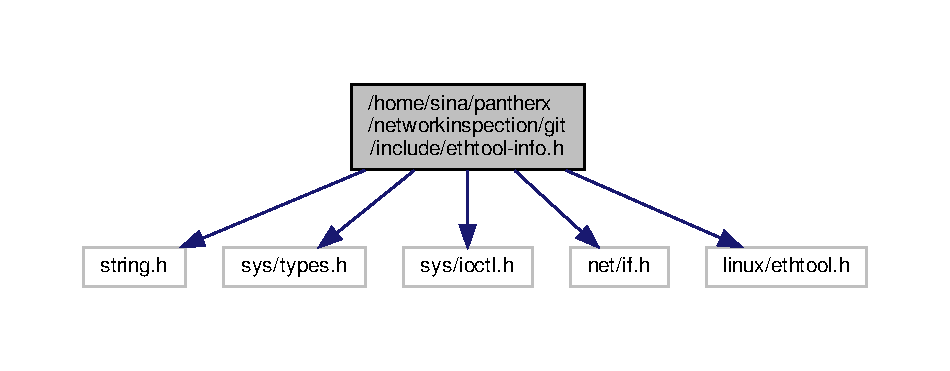
\includegraphics[width=350pt]{ethtool-info_8h__incl}
\end{center}
\end{figure}
This graph shows which files directly or indirectly include this file\+:\nopagebreak
\begin{figure}[H]
\begin{center}
\leavevmode
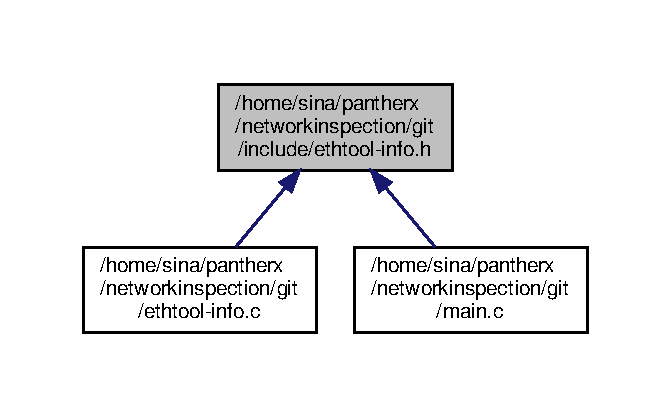
\includegraphics[width=322pt]{ethtool-info_8h__dep__incl}
\end{center}
\end{figure}
\subsection*{Classes}
\begin{DoxyCompactItemize}
\item 
struct \hyperlink{structcmd__context}{cmd\+\_\+context}
\end{DoxyCompactItemize}
\subsection*{Functions}
\begin{DoxyCompactItemize}
\item 
int \hyperlink{ethtool-info_8h_a6d58a8ebd8093edbe407365d8f3e93e5}{send\+\_\+ioctl} (struct \hyperlink{structcmd__context}{cmd\+\_\+context} $\ast$ctx, void $\ast$cmd)
\item 
int \hyperlink{ethtool-info_8h_a972c7feb6f25da37144ec7933d787147}{dump\+\_\+drvinfo} (struct ethtool\+\_\+drvinfo $\ast$info)
\item 
int \hyperlink{ethtool-info_8h_a92defcf2493dee90aeaac81e3b15572c}{do\+\_\+gdrv} (struct \hyperlink{structcmd__context}{cmd\+\_\+context} $\ast$ctx, struct ethtool\+\_\+drvinfo $\ast$drvinfo)
\item 
int \hyperlink{ethtool-info_8h_af4d8c485fa8cc199f6e1f27e949c9dc4}{get\+\_\+drv\+\_\+info} (char $\ast$ifa\+\_\+name, struct ethtool\+\_\+drvinfo $\ast$drvinfo)
\end{DoxyCompactItemize}


\subsection{Function Documentation}
\mbox{\Hypertarget{ethtool-info_8h_a92defcf2493dee90aeaac81e3b15572c}\label{ethtool-info_8h_a92defcf2493dee90aeaac81e3b15572c}} 
\index{ethtool-\/info.\+h@{ethtool-\/info.\+h}!do\+\_\+gdrv@{do\+\_\+gdrv}}
\index{do\+\_\+gdrv@{do\+\_\+gdrv}!ethtool-\/info.\+h@{ethtool-\/info.\+h}}
\subsubsection{\texorpdfstring{do\+\_\+gdrv()}{do\_gdrv()}}
{\footnotesize\ttfamily int do\+\_\+gdrv (\begin{DoxyParamCaption}\item[{struct \hyperlink{structcmd__context}{cmd\+\_\+context} $\ast$}]{ctx,  }\item[{struct ethtool\+\_\+drvinfo $\ast$}]{drvinfo }\end{DoxyParamCaption})}

\mbox{\Hypertarget{ethtool-info_8h_a972c7feb6f25da37144ec7933d787147}\label{ethtool-info_8h_a972c7feb6f25da37144ec7933d787147}} 
\index{ethtool-\/info.\+h@{ethtool-\/info.\+h}!dump\+\_\+drvinfo@{dump\+\_\+drvinfo}}
\index{dump\+\_\+drvinfo@{dump\+\_\+drvinfo}!ethtool-\/info.\+h@{ethtool-\/info.\+h}}
\subsubsection{\texorpdfstring{dump\+\_\+drvinfo()}{dump\_drvinfo()}}
{\footnotesize\ttfamily int dump\+\_\+drvinfo (\begin{DoxyParamCaption}\item[{struct ethtool\+\_\+drvinfo $\ast$}]{info }\end{DoxyParamCaption})}

\mbox{\Hypertarget{ethtool-info_8h_af4d8c485fa8cc199f6e1f27e949c9dc4}\label{ethtool-info_8h_af4d8c485fa8cc199f6e1f27e949c9dc4}} 
\index{ethtool-\/info.\+h@{ethtool-\/info.\+h}!get\+\_\+drv\+\_\+info@{get\+\_\+drv\+\_\+info}}
\index{get\+\_\+drv\+\_\+info@{get\+\_\+drv\+\_\+info}!ethtool-\/info.\+h@{ethtool-\/info.\+h}}
\subsubsection{\texorpdfstring{get\+\_\+drv\+\_\+info()}{get\_drv\_info()}}
{\footnotesize\ttfamily int get\+\_\+drv\+\_\+info (\begin{DoxyParamCaption}\item[{char $\ast$}]{ifa\+\_\+name,  }\item[{struct ethtool\+\_\+drvinfo $\ast$}]{drvinfo }\end{DoxyParamCaption})}

\mbox{\Hypertarget{ethtool-info_8h_a6d58a8ebd8093edbe407365d8f3e93e5}\label{ethtool-info_8h_a6d58a8ebd8093edbe407365d8f3e93e5}} 
\index{ethtool-\/info.\+h@{ethtool-\/info.\+h}!send\+\_\+ioctl@{send\+\_\+ioctl}}
\index{send\+\_\+ioctl@{send\+\_\+ioctl}!ethtool-\/info.\+h@{ethtool-\/info.\+h}}
\subsubsection{\texorpdfstring{send\+\_\+ioctl()}{send\_ioctl()}}
{\footnotesize\ttfamily int send\+\_\+ioctl (\begin{DoxyParamCaption}\item[{struct \hyperlink{structcmd__context}{cmd\+\_\+context} $\ast$}]{ctx,  }\item[{void $\ast$}]{cmd }\end{DoxyParamCaption})}


\hypertarget{gnode-object_8h}{}\section{/home/sina/pantherx/networkinspection/git/include/gnode-\/object.h File Reference}
\label{gnode-object_8h}\index{/home/sina/pantherx/networkinspection/git/include/gnode-\/object.\+h@{/home/sina/pantherx/networkinspection/git/include/gnode-\/object.\+h}}
{\ttfamily \#include $<$glib.\+h$>$}\newline
{\ttfamily \#include $<$stdint.\+h$>$}\newline
{\ttfamily \#include $<$json-\/c/json.\+h$>$}\newline
{\ttfamily \#include $<$linux/wireless.\+h$>$}\newline
{\ttfamily \#include $<$linux/limits.\+h$>$}\newline
Include dependency graph for gnode-\/object.h\+:\nopagebreak
\begin{figure}[H]
\begin{center}
\leavevmode
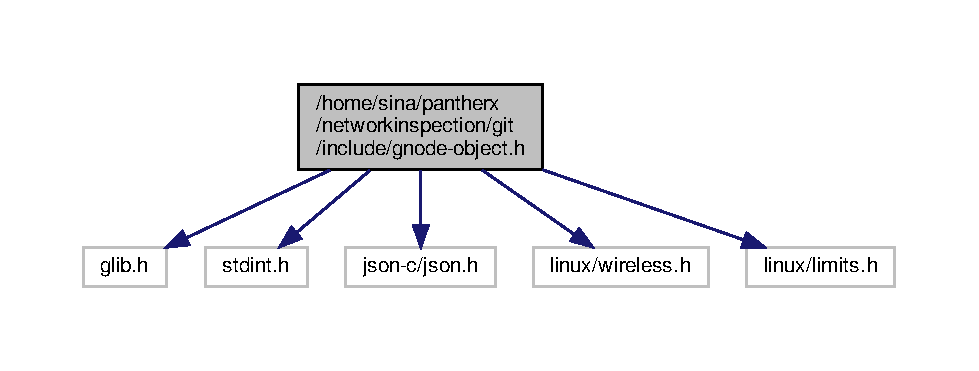
\includegraphics[width=350pt]{gnode-object_8h__incl}
\end{center}
\end{figure}
This graph shows which files directly or indirectly include this file\+:\nopagebreak
\begin{figure}[H]
\begin{center}
\leavevmode
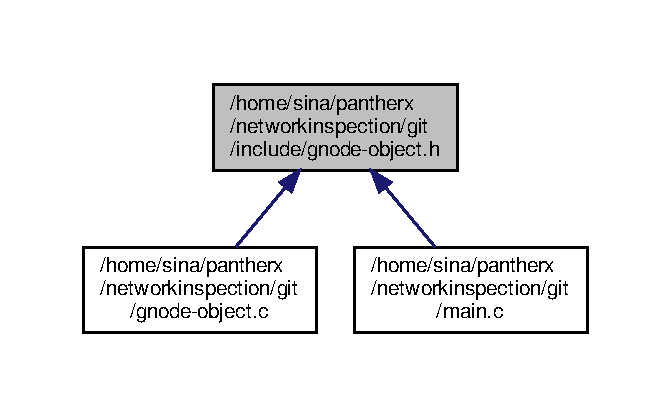
\includegraphics[width=322pt]{gnode-object_8h__dep__incl}
\end{center}
\end{figure}
\subsection*{Classes}
\begin{DoxyCompactItemize}
\item 
struct \hyperlink{structnet__device}{net\+\_\+device}
\end{DoxyCompactItemize}
\subsection*{Macros}
\begin{DoxyCompactItemize}
\item 
\#define \hyperlink{gnode-object_8h_a92eeaa07ea1bf740872e6f0fc1cf0caf}{N\+E\+T\+D\+E\+V\+I\+CE}(o)~(\hyperlink{gnode-object_8h_ab9c23d3a2ba4d9157b5ab053f61388dc}{Net\+Device}$\ast$)(o)
\end{DoxyCompactItemize}
\subsection*{Typedefs}
\begin{DoxyCompactItemize}
\item 
typedef struct \hyperlink{structnet__device}{net\+\_\+device} \hyperlink{gnode-object_8h_ab9c23d3a2ba4d9157b5ab053f61388dc}{Net\+Device}
\end{DoxyCompactItemize}
\subsection*{Functions}
\begin{DoxyCompactItemize}
\item 
\hyperlink{gnode-object_8h_ab9c23d3a2ba4d9157b5ab053f61388dc}{Net\+Device} $\ast$ \hyperlink{gnode-object_8h_ae666b3f20895e60917e691c81d464235}{net\+\_\+device\+\_\+new} ()
\item 
void \hyperlink{gnode-object_8h_af75477fcbe781bc0b17c75c1ad6d1606}{net\+\_\+device\+\_\+free} (\hyperlink{gnode-object_8h_ab9c23d3a2ba4d9157b5ab053f61388dc}{Net\+Device} $\ast$nd)
\item 
gboolean \hyperlink{gnode-object_8h_acde5d3e413f355d1b912f0dcb9d4cdc1}{traverse\+\_\+json\+\_\+func} (G\+Node $\ast$node, gpointer data)
\item 
gboolean \hyperlink{gnode-object_8h_a0d906716c0b2c59e34bff01153dc23d2}{traverse\+\_\+json\+\_\+array\+\_\+func} (G\+Node $\ast$node, gpointer data)
\end{DoxyCompactItemize}


\subsection{Macro Definition Documentation}
\mbox{\Hypertarget{gnode-object_8h_a92eeaa07ea1bf740872e6f0fc1cf0caf}\label{gnode-object_8h_a92eeaa07ea1bf740872e6f0fc1cf0caf}} 
\index{gnode-\/object.\+h@{gnode-\/object.\+h}!N\+E\+T\+D\+E\+V\+I\+CE@{N\+E\+T\+D\+E\+V\+I\+CE}}
\index{N\+E\+T\+D\+E\+V\+I\+CE@{N\+E\+T\+D\+E\+V\+I\+CE}!gnode-\/object.\+h@{gnode-\/object.\+h}}
\subsubsection{\texorpdfstring{N\+E\+T\+D\+E\+V\+I\+CE}{NETDEVICE}}
{\footnotesize\ttfamily \#define N\+E\+T\+D\+E\+V\+I\+CE(\begin{DoxyParamCaption}\item[{}]{o }\end{DoxyParamCaption})~(\hyperlink{gnode-object_8h_ab9c23d3a2ba4d9157b5ab053f61388dc}{Net\+Device}$\ast$)(o)}



\subsection{Typedef Documentation}
\mbox{\Hypertarget{gnode-object_8h_ab9c23d3a2ba4d9157b5ab053f61388dc}\label{gnode-object_8h_ab9c23d3a2ba4d9157b5ab053f61388dc}} 
\index{gnode-\/object.\+h@{gnode-\/object.\+h}!Net\+Device@{Net\+Device}}
\index{Net\+Device@{Net\+Device}!gnode-\/object.\+h@{gnode-\/object.\+h}}
\subsubsection{\texorpdfstring{Net\+Device}{NetDevice}}
{\footnotesize\ttfamily typedef struct \hyperlink{structnet__device}{net\+\_\+device}  \hyperlink{gnode-object_8h_ab9c23d3a2ba4d9157b5ab053f61388dc}{Net\+Device}}



\subsection{Function Documentation}
\mbox{\Hypertarget{gnode-object_8h_af75477fcbe781bc0b17c75c1ad6d1606}\label{gnode-object_8h_af75477fcbe781bc0b17c75c1ad6d1606}} 
\index{gnode-\/object.\+h@{gnode-\/object.\+h}!net\+\_\+device\+\_\+free@{net\+\_\+device\+\_\+free}}
\index{net\+\_\+device\+\_\+free@{net\+\_\+device\+\_\+free}!gnode-\/object.\+h@{gnode-\/object.\+h}}
\subsubsection{\texorpdfstring{net\+\_\+device\+\_\+free()}{net\_device\_free()}}
{\footnotesize\ttfamily void net\+\_\+device\+\_\+free (\begin{DoxyParamCaption}\item[{\hyperlink{gnode-object_8h_ab9c23d3a2ba4d9157b5ab053f61388dc}{Net\+Device} $\ast$}]{nd }\end{DoxyParamCaption})}

\mbox{\Hypertarget{gnode-object_8h_ae666b3f20895e60917e691c81d464235}\label{gnode-object_8h_ae666b3f20895e60917e691c81d464235}} 
\index{gnode-\/object.\+h@{gnode-\/object.\+h}!net\+\_\+device\+\_\+new@{net\+\_\+device\+\_\+new}}
\index{net\+\_\+device\+\_\+new@{net\+\_\+device\+\_\+new}!gnode-\/object.\+h@{gnode-\/object.\+h}}
\subsubsection{\texorpdfstring{net\+\_\+device\+\_\+new()}{net\_device\_new()}}
{\footnotesize\ttfamily \hyperlink{gnode-object_8h_ab9c23d3a2ba4d9157b5ab053f61388dc}{Net\+Device}$\ast$ net\+\_\+device\+\_\+new (\begin{DoxyParamCaption}{ }\end{DoxyParamCaption})}

\mbox{\Hypertarget{gnode-object_8h_a0d906716c0b2c59e34bff01153dc23d2}\label{gnode-object_8h_a0d906716c0b2c59e34bff01153dc23d2}} 
\index{gnode-\/object.\+h@{gnode-\/object.\+h}!traverse\+\_\+json\+\_\+array\+\_\+func@{traverse\+\_\+json\+\_\+array\+\_\+func}}
\index{traverse\+\_\+json\+\_\+array\+\_\+func@{traverse\+\_\+json\+\_\+array\+\_\+func}!gnode-\/object.\+h@{gnode-\/object.\+h}}
\subsubsection{\texorpdfstring{traverse\+\_\+json\+\_\+array\+\_\+func()}{traverse\_json\_array\_func()}}
{\footnotesize\ttfamily gboolean traverse\+\_\+json\+\_\+array\+\_\+func (\begin{DoxyParamCaption}\item[{G\+Node $\ast$}]{node,  }\item[{gpointer}]{data }\end{DoxyParamCaption})}

\mbox{\Hypertarget{gnode-object_8h_acde5d3e413f355d1b912f0dcb9d4cdc1}\label{gnode-object_8h_acde5d3e413f355d1b912f0dcb9d4cdc1}} 
\index{gnode-\/object.\+h@{gnode-\/object.\+h}!traverse\+\_\+json\+\_\+func@{traverse\+\_\+json\+\_\+func}}
\index{traverse\+\_\+json\+\_\+func@{traverse\+\_\+json\+\_\+func}!gnode-\/object.\+h@{gnode-\/object.\+h}}
\subsubsection{\texorpdfstring{traverse\+\_\+json\+\_\+func()}{traverse\_json\_func()}}
{\footnotesize\ttfamily gboolean traverse\+\_\+json\+\_\+func (\begin{DoxyParamCaption}\item[{G\+Node $\ast$}]{node,  }\item[{gpointer}]{data }\end{DoxyParamCaption})}


\hypertarget{public-ip_8h}{}\section{/home/sina/pantherx/networkinspection/git/include/public-\/ip.h File Reference}
\label{public-ip_8h}\index{/home/sina/pantherx/networkinspection/git/include/public-\/ip.\+h@{/home/sina/pantherx/networkinspection/git/include/public-\/ip.\+h}}
{\ttfamily \#include $<$stdlib.\+h$>$}\newline
{\ttfamily \#include $<$route-\/tree.\+h$>$}\newline
Include dependency graph for public-\/ip.h\+:\nopagebreak
\begin{figure}[H]
\begin{center}
\leavevmode
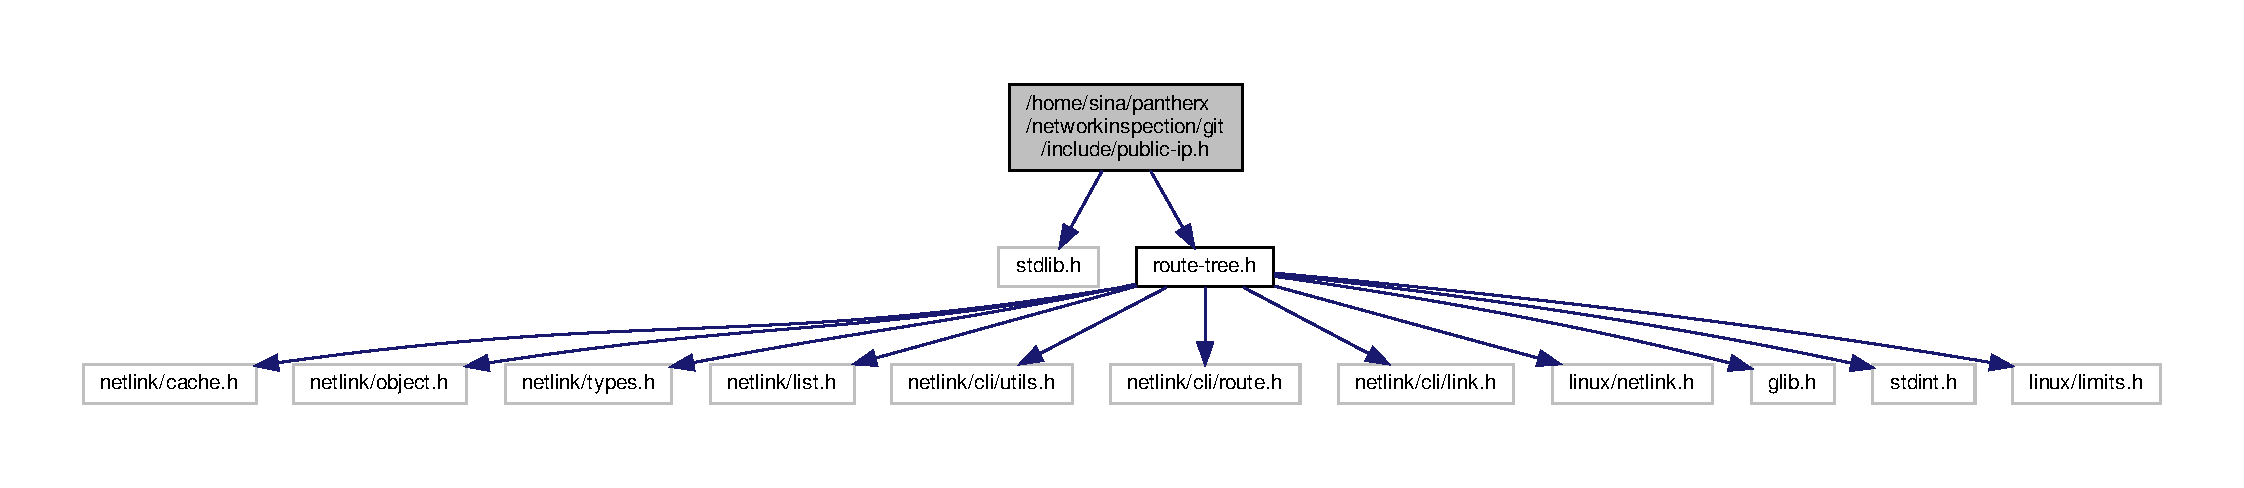
\includegraphics[width=350pt]{public-ip_8h__incl}
\end{center}
\end{figure}
This graph shows which files directly or indirectly include this file\+:\nopagebreak
\begin{figure}[H]
\begin{center}
\leavevmode
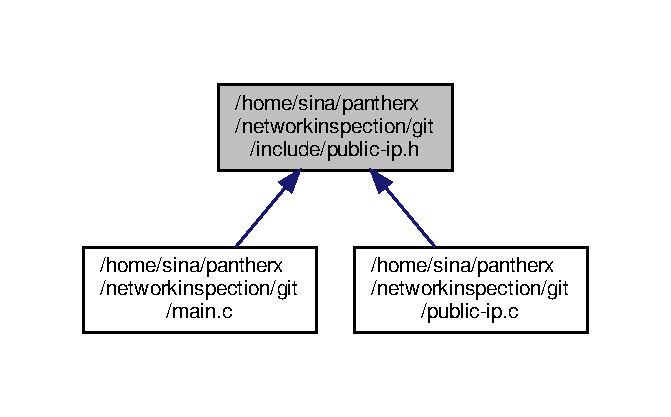
\includegraphics[width=322pt]{public-ip_8h__dep__incl}
\end{center}
\end{figure}
\subsection*{Classes}
\begin{DoxyCompactItemize}
\item 
struct \hyperlink{structurl__data}{url\+\_\+data}
\end{DoxyCompactItemize}
\subsection*{Functions}
\begin{DoxyCompactItemize}
\item 
void \hyperlink{public-ip_8h_a343631cf6f2ceb1736d8b227c2cf76d3}{get\+\_\+public\+\_\+ip} (char if\+\_\+names\mbox{[}\hyperlink{route-tree_8h_a5f66955385e84e67789d731b5cad24c7}{M\+A\+X\+\_\+\+P\+H\+Y\+S\+\_\+\+I\+FS}\mbox{]}\mbox{[}16\mbox{]}, int if\+\_\+number, char if\+\_\+public\+\_\+ips\mbox{[}\hyperlink{route-tree_8h_a5f66955385e84e67789d731b5cad24c7}{M\+A\+X\+\_\+\+P\+H\+Y\+S\+\_\+\+I\+FS}\mbox{]}\mbox{[}40\mbox{]})
\end{DoxyCompactItemize}


\subsection{Function Documentation}
\mbox{\Hypertarget{public-ip_8h_a343631cf6f2ceb1736d8b227c2cf76d3}\label{public-ip_8h_a343631cf6f2ceb1736d8b227c2cf76d3}} 
\index{public-\/ip.\+h@{public-\/ip.\+h}!get\+\_\+public\+\_\+ip@{get\+\_\+public\+\_\+ip}}
\index{get\+\_\+public\+\_\+ip@{get\+\_\+public\+\_\+ip}!public-\/ip.\+h@{public-\/ip.\+h}}
\subsubsection{\texorpdfstring{get\+\_\+public\+\_\+ip()}{get\_public\_ip()}}
{\footnotesize\ttfamily void get\+\_\+public\+\_\+ip (\begin{DoxyParamCaption}\item[{char}]{if\+\_\+names\mbox{[}\+M\+A\+X\+\_\+\+P\+H\+Y\+S\+\_\+\+I\+F\+S\mbox{]}\mbox{[}16\mbox{]},  }\item[{int}]{if\+\_\+number,  }\item[{char}]{if\+\_\+public\+\_\+ips\mbox{[}\+M\+A\+X\+\_\+\+P\+H\+Y\+S\+\_\+\+I\+F\+S\mbox{]}\mbox{[}40\mbox{]} }\end{DoxyParamCaption})}


\hypertarget{route-tree_8h}{}\section{/home/sina/pantherx/networkinspection/git/include/route-\/tree.h File Reference}
\label{route-tree_8h}\index{/home/sina/pantherx/networkinspection/git/include/route-\/tree.\+h@{/home/sina/pantherx/networkinspection/git/include/route-\/tree.\+h}}
{\ttfamily \#include $<$netlink/cache.\+h$>$}\newline
{\ttfamily \#include $<$netlink/object.\+h$>$}\newline
{\ttfamily \#include $<$netlink/types.\+h$>$}\newline
{\ttfamily \#include $<$netlink/list.\+h$>$}\newline
{\ttfamily \#include $<$netlink/cli/utils.\+h$>$}\newline
{\ttfamily \#include $<$netlink/cli/route.\+h$>$}\newline
{\ttfamily \#include $<$netlink/cli/link.\+h$>$}\newline
{\ttfamily \#include $<$linux/netlink.\+h$>$}\newline
{\ttfamily \#include $<$glib.\+h$>$}\newline
{\ttfamily \#include $<$stdint.\+h$>$}\newline
{\ttfamily \#include $<$linux/limits.\+h$>$}\newline
Include dependency graph for route-\/tree.h\+:\nopagebreak
\begin{figure}[H]
\begin{center}
\leavevmode
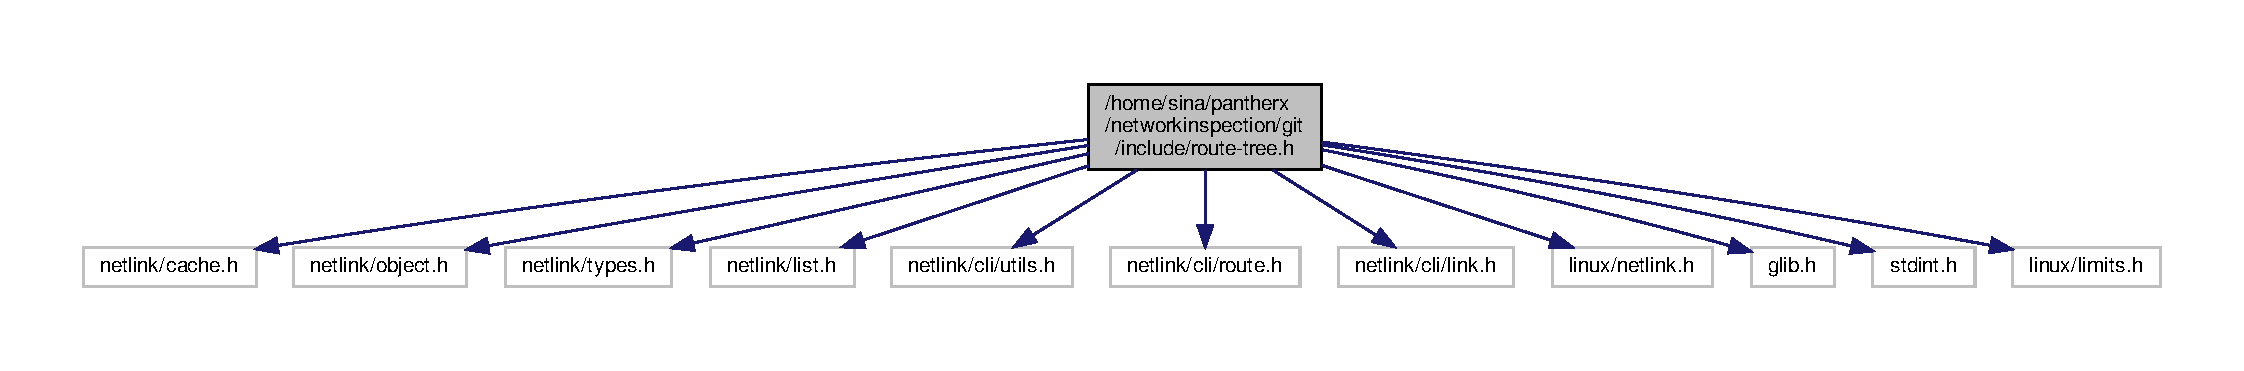
\includegraphics[width=350pt]{route-tree_8h__incl}
\end{center}
\end{figure}
This graph shows which files directly or indirectly include this file\+:\nopagebreak
\begin{figure}[H]
\begin{center}
\leavevmode
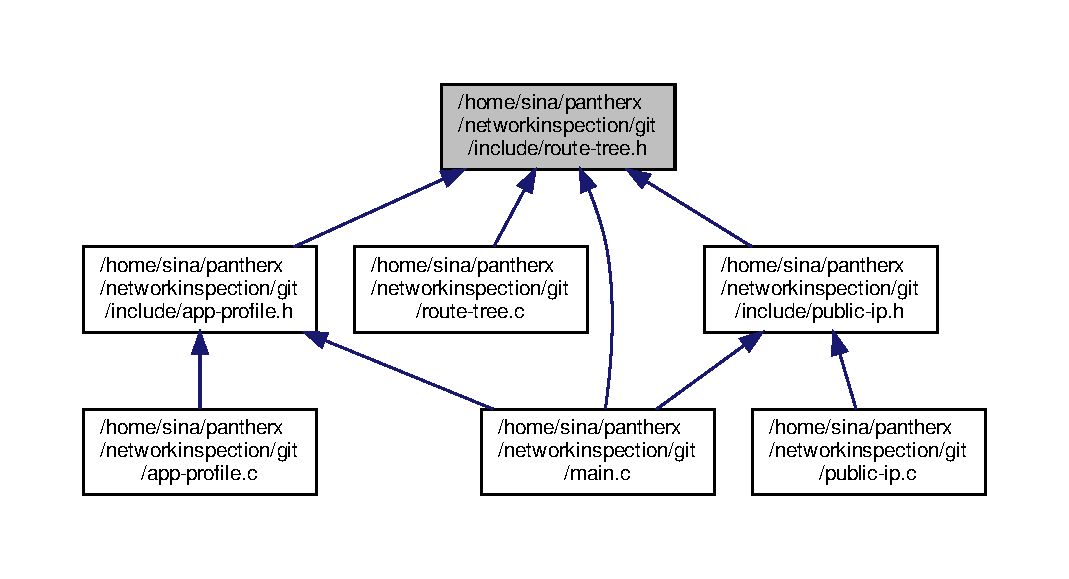
\includegraphics[width=350pt]{route-tree_8h__dep__incl}
\end{center}
\end{figure}
\subsection*{Classes}
\begin{DoxyCompactItemize}
\item 
struct \hyperlink{structvpnmethod}{vpnmethod}
\begin{DoxyCompactList}\small\item\em the struct to be put both V\+PN method and name together \end{DoxyCompactList}\item 
struct \hyperlink{structroute__node}{route\+\_\+node}
\begin{DoxyCompactList}\small\item\em the extracted information of a node in a kernel route table \end{DoxyCompactList}\end{DoxyCompactItemize}
\subsection*{Macros}
\begin{DoxyCompactItemize}
\item 
\#define \hyperlink{route-tree_8h_a8e1da3af3417de420798c8b448b6a8cb}{M\+A\+X\+\_\+\+R\+O\+O\+T\+S\+\_\+\+N\+U\+M\+B\+ER}~10
\item 
\#define \hyperlink{route-tree_8h_a5f66955385e84e67789d731b5cad24c7}{M\+A\+X\+\_\+\+P\+H\+Y\+S\+\_\+\+I\+FS}~\hyperlink{route-tree_8h_a8e1da3af3417de420798c8b448b6a8cb}{M\+A\+X\+\_\+\+R\+O\+O\+T\+S\+\_\+\+N\+U\+M\+B\+ER}
\item 
\#define \hyperlink{route-tree_8h_a82e5e4b05dda947b534dc0941ad418ba}{M\+A\+X\+\_\+\+T\+A\+P\+\_\+\+I\+FS}~10
\item 
\#define \hyperlink{route-tree_8h_a0d314d64c79d675bd2614b20e738d527}{M\+A\+X\+\_\+\+T\+U\+N\+\_\+\+I\+FS}~10
\item 
\#define \hyperlink{route-tree_8h_a77ed9a5f9670b7a2d69c376d1199eddf}{M\+A\+X\+\_\+\+V\+P\+N\+\_\+\+N\+A\+ME}~50
\item 
\#define \hyperlink{route-tree_8h_ab6867a2365732ebd41ddf7459525d032}{M\+A\+X\+\_\+\+V\+P\+N\+\_\+\+P\+R\+O\+F\+I\+L\+E\+\_\+\+N\+A\+ME}~N\+A\+M\+E\+\_\+\+M\+AX
\item 
\#define \hyperlink{route-tree_8h_ab4431a377dee3e169cfe060fe7666758}{R\+O\+U\+T\+E\+N\+O\+DE}(o)~(\hyperlink{route-tree_8h_a1296be44c6672a1adb94ba6dc416682c}{Route\+Node}$\ast$)(o)
\item 
\#define \hyperlink{route-tree_8h_a58aa26c75d296ca73e2bca481e6e036f}{V\+P\+N\+M\+E\+T\+H\+OD}(o)~(\hyperlink{route-tree_8h_a1034dd038389279bf422489d4d99d43a}{Vpn\+Method}$\ast$)(o)
\end{DoxyCompactItemize}
\subsection*{Typedefs}
\begin{DoxyCompactItemize}
\item 
typedef struct \hyperlink{structvpnmethod}{vpnmethod} \hyperlink{route-tree_8h_a1034dd038389279bf422489d4d99d43a}{Vpn\+Method}
\begin{DoxyCompactList}\small\item\em the struct to be put both V\+PN method and name together \end{DoxyCompactList}\item 
typedef struct \hyperlink{structroute__node}{route\+\_\+node} \hyperlink{route-tree_8h_a1296be44c6672a1adb94ba6dc416682c}{Route\+Node}
\begin{DoxyCompactList}\small\item\em the extracted information of a node in a kernel route table \end{DoxyCompactList}\end{DoxyCompactItemize}
\subsection*{Enumerations}
\begin{DoxyCompactItemize}
\item 
enum \hyperlink{route-tree_8h_a5b876670828c4e38106ba1c6d91024b7}{V\+P\+N\+\_\+\+M\+E\+T\+H\+O\+DS} \{ \newline
\hyperlink{route-tree_8h_a5b876670828c4e38106ba1c6d91024b7ab1ae185eb0d77c55896e16a13cc83fcd}{O\+P\+E\+N\+V\+PN}, 
\hyperlink{route-tree_8h_a5b876670828c4e38106ba1c6d91024b7a16a826749e7c59a1ac398c5fea811044}{W\+I\+R\+E\+G\+U\+A\+RD}, 
\hyperlink{route-tree_8h_a5b876670828c4e38106ba1c6d91024b7ac610d0f8eb941cb8d8a5a1e30f60ea1b}{A\+N\+Y\+C\+O\+N\+N\+E\+CT}, 
\hyperlink{route-tree_8h_a5b876670828c4e38106ba1c6d91024b7a12890d8b7f1c543c687d8d72ce33d749}{V\+P\+N\+\_\+\+M\+E\+T\+H\+O\+D\+S\+\_\+\+N\+U\+M\+B\+E\+RS}, 
\newline
\hyperlink{route-tree_8h_a5b876670828c4e38106ba1c6d91024b7a096310080aa42637b2920b2e9e78aacd}{N\+O\+\_\+\+V\+P\+N\+\_\+\+M\+E\+T\+H\+OD}, 
\hyperlink{route-tree_8h_a5b876670828c4e38106ba1c6d91024b7a7df79fc150333242d7a3df021b1b2206}{V\+P\+N\+\_\+\+M\+E\+T\+H\+O\+D\+\_\+\+U\+N\+K\+N\+O\+WN}
 \}\begin{DoxyCompactList}\small\item\em the supported methods for running V\+PN on a machine \end{DoxyCompactList}
\end{DoxyCompactItemize}
\subsection*{Functions}
\begin{DoxyCompactItemize}
\item 
\hyperlink{route-tree_8h_a1034dd038389279bf422489d4d99d43a}{Vpn\+Method} $\ast$ \hyperlink{route-tree_8h_a3ccbf1b413fe282c1490701f739273a8}{vpn\+\_\+method\+\_\+new} ()
\begin{DoxyCompactList}\small\item\em creates a new Vpn\+Method object \end{DoxyCompactList}\item 
void \hyperlink{route-tree_8h_a24c2b4e2f6cd24a639b2fe63bb48f48e}{vpn\+\_\+method\+\_\+free} (\hyperlink{route-tree_8h_a1034dd038389279bf422489d4d99d43a}{Vpn\+Method} $\ast$vm)
\begin{DoxyCompactList}\small\item\em destroys a Vpn\+Method object \end{DoxyCompactList}\item 
\hyperlink{route-tree_8h_a1034dd038389279bf422489d4d99d43a}{Vpn\+Method} $\ast$ \hyperlink{route-tree_8h_a267529614de44218b8187f3ac46ce46f}{detect\+\_\+vpn\+\_\+method} ()
\begin{DoxyCompactList}\small\item\em detect V\+PN method based on kernel routing pattern \end{DoxyCompactList}\item 
\hyperlink{route-tree_8h_a1296be44c6672a1adb94ba6dc416682c}{Route\+Node} $\ast$ \hyperlink{route-tree_8h_a941ed51572db1d1d4720f8a329dd0d8b}{route\+\_\+node\+\_\+new} ()
\begin{DoxyCompactList}\small\item\em creates a new Route\+Node object \end{DoxyCompactList}\item 
void \hyperlink{route-tree_8h_a1b80d492072ee18f906bdd2fbaad9b4b}{route\+\_\+node\+\_\+free} (\hyperlink{route-tree_8h_a1296be44c6672a1adb94ba6dc416682c}{Route\+Node} $\ast$nd)
\begin{DoxyCompactList}\small\item\em destroys a Route\+Node object \end{DoxyCompactList}\item 
int \hyperlink{route-tree_8h_a5a490e2e29be18ae630572e3776539af}{analyze\+\_\+kernel\+\_\+route} (G\+Node $\ast$kernel\+\_\+route\+\_\+roots\mbox{[}\hyperlink{route-tree_8h_a8e1da3af3417de420798c8b448b6a8cb}{M\+A\+X\+\_\+\+R\+O\+O\+T\+S\+\_\+\+N\+U\+M\+B\+ER}\mbox{]}, int $\ast$kernel\+\_\+roots, enum \hyperlink{route-tree_8h_a5b876670828c4e38106ba1c6d91024b7}{V\+P\+N\+\_\+\+M\+E\+T\+H\+O\+DS} vpn\+\_\+method)
\begin{DoxyCompactList}\small\item\em detect V\+PN method based on kernel routing pattern \end{DoxyCompactList}\item 
G\+Node $\ast$ \hyperlink{route-tree_8h_a77affcaa875961893c05c7e211678ed1}{get\+\_\+kernel\+\_\+route\+\_\+node} (G\+Node $\ast$kernel\+\_\+route\+\_\+roots\mbox{[}\hyperlink{route-tree_8h_a8e1da3af3417de420798c8b448b6a8cb}{M\+A\+X\+\_\+\+R\+O\+O\+T\+S\+\_\+\+N\+U\+M\+B\+ER}\mbox{]}, int roots, char $\ast$ifa\+\_\+name)
\begin{DoxyCompactList}\small\item\em find the node with the interface name within the jungle of kernel route table \end{DoxyCompactList}\end{DoxyCompactItemize}


\subsection{Macro Definition Documentation}
\mbox{\Hypertarget{route-tree_8h_a5f66955385e84e67789d731b5cad24c7}\label{route-tree_8h_a5f66955385e84e67789d731b5cad24c7}} 
\index{route-\/tree.\+h@{route-\/tree.\+h}!M\+A\+X\+\_\+\+P\+H\+Y\+S\+\_\+\+I\+FS@{M\+A\+X\+\_\+\+P\+H\+Y\+S\+\_\+\+I\+FS}}
\index{M\+A\+X\+\_\+\+P\+H\+Y\+S\+\_\+\+I\+FS@{M\+A\+X\+\_\+\+P\+H\+Y\+S\+\_\+\+I\+FS}!route-\/tree.\+h@{route-\/tree.\+h}}
\subsubsection{\texorpdfstring{M\+A\+X\+\_\+\+P\+H\+Y\+S\+\_\+\+I\+FS}{MAX\_PHYS\_IFS}}
{\footnotesize\ttfamily \#define M\+A\+X\+\_\+\+P\+H\+Y\+S\+\_\+\+I\+FS~\hyperlink{route-tree_8h_a8e1da3af3417de420798c8b448b6a8cb}{M\+A\+X\+\_\+\+R\+O\+O\+T\+S\+\_\+\+N\+U\+M\+B\+ER}}

\mbox{\Hypertarget{route-tree_8h_a8e1da3af3417de420798c8b448b6a8cb}\label{route-tree_8h_a8e1da3af3417de420798c8b448b6a8cb}} 
\index{route-\/tree.\+h@{route-\/tree.\+h}!M\+A\+X\+\_\+\+R\+O\+O\+T\+S\+\_\+\+N\+U\+M\+B\+ER@{M\+A\+X\+\_\+\+R\+O\+O\+T\+S\+\_\+\+N\+U\+M\+B\+ER}}
\index{M\+A\+X\+\_\+\+R\+O\+O\+T\+S\+\_\+\+N\+U\+M\+B\+ER@{M\+A\+X\+\_\+\+R\+O\+O\+T\+S\+\_\+\+N\+U\+M\+B\+ER}!route-\/tree.\+h@{route-\/tree.\+h}}
\subsubsection{\texorpdfstring{M\+A\+X\+\_\+\+R\+O\+O\+T\+S\+\_\+\+N\+U\+M\+B\+ER}{MAX\_ROOTS\_NUMBER}}
{\footnotesize\ttfamily \#define M\+A\+X\+\_\+\+R\+O\+O\+T\+S\+\_\+\+N\+U\+M\+B\+ER~10}

\mbox{\Hypertarget{route-tree_8h_a82e5e4b05dda947b534dc0941ad418ba}\label{route-tree_8h_a82e5e4b05dda947b534dc0941ad418ba}} 
\index{route-\/tree.\+h@{route-\/tree.\+h}!M\+A\+X\+\_\+\+T\+A\+P\+\_\+\+I\+FS@{M\+A\+X\+\_\+\+T\+A\+P\+\_\+\+I\+FS}}
\index{M\+A\+X\+\_\+\+T\+A\+P\+\_\+\+I\+FS@{M\+A\+X\+\_\+\+T\+A\+P\+\_\+\+I\+FS}!route-\/tree.\+h@{route-\/tree.\+h}}
\subsubsection{\texorpdfstring{M\+A\+X\+\_\+\+T\+A\+P\+\_\+\+I\+FS}{MAX\_TAP\_IFS}}
{\footnotesize\ttfamily \#define M\+A\+X\+\_\+\+T\+A\+P\+\_\+\+I\+FS~10}

\mbox{\Hypertarget{route-tree_8h_a0d314d64c79d675bd2614b20e738d527}\label{route-tree_8h_a0d314d64c79d675bd2614b20e738d527}} 
\index{route-\/tree.\+h@{route-\/tree.\+h}!M\+A\+X\+\_\+\+T\+U\+N\+\_\+\+I\+FS@{M\+A\+X\+\_\+\+T\+U\+N\+\_\+\+I\+FS}}
\index{M\+A\+X\+\_\+\+T\+U\+N\+\_\+\+I\+FS@{M\+A\+X\+\_\+\+T\+U\+N\+\_\+\+I\+FS}!route-\/tree.\+h@{route-\/tree.\+h}}
\subsubsection{\texorpdfstring{M\+A\+X\+\_\+\+T\+U\+N\+\_\+\+I\+FS}{MAX\_TUN\_IFS}}
{\footnotesize\ttfamily \#define M\+A\+X\+\_\+\+T\+U\+N\+\_\+\+I\+FS~10}

\mbox{\Hypertarget{route-tree_8h_a77ed9a5f9670b7a2d69c376d1199eddf}\label{route-tree_8h_a77ed9a5f9670b7a2d69c376d1199eddf}} 
\index{route-\/tree.\+h@{route-\/tree.\+h}!M\+A\+X\+\_\+\+V\+P\+N\+\_\+\+N\+A\+ME@{M\+A\+X\+\_\+\+V\+P\+N\+\_\+\+N\+A\+ME}}
\index{M\+A\+X\+\_\+\+V\+P\+N\+\_\+\+N\+A\+ME@{M\+A\+X\+\_\+\+V\+P\+N\+\_\+\+N\+A\+ME}!route-\/tree.\+h@{route-\/tree.\+h}}
\subsubsection{\texorpdfstring{M\+A\+X\+\_\+\+V\+P\+N\+\_\+\+N\+A\+ME}{MAX\_VPN\_NAME}}
{\footnotesize\ttfamily \#define M\+A\+X\+\_\+\+V\+P\+N\+\_\+\+N\+A\+ME~50}

\mbox{\Hypertarget{route-tree_8h_ab6867a2365732ebd41ddf7459525d032}\label{route-tree_8h_ab6867a2365732ebd41ddf7459525d032}} 
\index{route-\/tree.\+h@{route-\/tree.\+h}!M\+A\+X\+\_\+\+V\+P\+N\+\_\+\+P\+R\+O\+F\+I\+L\+E\+\_\+\+N\+A\+ME@{M\+A\+X\+\_\+\+V\+P\+N\+\_\+\+P\+R\+O\+F\+I\+L\+E\+\_\+\+N\+A\+ME}}
\index{M\+A\+X\+\_\+\+V\+P\+N\+\_\+\+P\+R\+O\+F\+I\+L\+E\+\_\+\+N\+A\+ME@{M\+A\+X\+\_\+\+V\+P\+N\+\_\+\+P\+R\+O\+F\+I\+L\+E\+\_\+\+N\+A\+ME}!route-\/tree.\+h@{route-\/tree.\+h}}
\subsubsection{\texorpdfstring{M\+A\+X\+\_\+\+V\+P\+N\+\_\+\+P\+R\+O\+F\+I\+L\+E\+\_\+\+N\+A\+ME}{MAX\_VPN\_PROFILE\_NAME}}
{\footnotesize\ttfamily \#define M\+A\+X\+\_\+\+V\+P\+N\+\_\+\+P\+R\+O\+F\+I\+L\+E\+\_\+\+N\+A\+ME~N\+A\+M\+E\+\_\+\+M\+AX}

\mbox{\Hypertarget{route-tree_8h_ab4431a377dee3e169cfe060fe7666758}\label{route-tree_8h_ab4431a377dee3e169cfe060fe7666758}} 
\index{route-\/tree.\+h@{route-\/tree.\+h}!R\+O\+U\+T\+E\+N\+O\+DE@{R\+O\+U\+T\+E\+N\+O\+DE}}
\index{R\+O\+U\+T\+E\+N\+O\+DE@{R\+O\+U\+T\+E\+N\+O\+DE}!route-\/tree.\+h@{route-\/tree.\+h}}
\subsubsection{\texorpdfstring{R\+O\+U\+T\+E\+N\+O\+DE}{ROUTENODE}}
{\footnotesize\ttfamily \#define R\+O\+U\+T\+E\+N\+O\+DE(\begin{DoxyParamCaption}\item[{}]{o }\end{DoxyParamCaption})~(\hyperlink{route-tree_8h_a1296be44c6672a1adb94ba6dc416682c}{Route\+Node}$\ast$)(o)}

\mbox{\Hypertarget{route-tree_8h_a58aa26c75d296ca73e2bca481e6e036f}\label{route-tree_8h_a58aa26c75d296ca73e2bca481e6e036f}} 
\index{route-\/tree.\+h@{route-\/tree.\+h}!V\+P\+N\+M\+E\+T\+H\+OD@{V\+P\+N\+M\+E\+T\+H\+OD}}
\index{V\+P\+N\+M\+E\+T\+H\+OD@{V\+P\+N\+M\+E\+T\+H\+OD}!route-\/tree.\+h@{route-\/tree.\+h}}
\subsubsection{\texorpdfstring{V\+P\+N\+M\+E\+T\+H\+OD}{VPNMETHOD}}
{\footnotesize\ttfamily \#define V\+P\+N\+M\+E\+T\+H\+OD(\begin{DoxyParamCaption}\item[{}]{o }\end{DoxyParamCaption})~(\hyperlink{route-tree_8h_a1034dd038389279bf422489d4d99d43a}{Vpn\+Method}$\ast$)(o)}



\subsection{Typedef Documentation}
\mbox{\Hypertarget{route-tree_8h_a1296be44c6672a1adb94ba6dc416682c}\label{route-tree_8h_a1296be44c6672a1adb94ba6dc416682c}} 
\index{route-\/tree.\+h@{route-\/tree.\+h}!Route\+Node@{Route\+Node}}
\index{Route\+Node@{Route\+Node}!route-\/tree.\+h@{route-\/tree.\+h}}
\subsubsection{\texorpdfstring{Route\+Node}{RouteNode}}
{\footnotesize\ttfamily typedef struct \hyperlink{structroute__node}{route\+\_\+node} \hyperlink{route-tree_8h_a1296be44c6672a1adb94ba6dc416682c}{Route\+Node}}



the extracted information of a node in a kernel route table 

\mbox{\Hypertarget{route-tree_8h_a1034dd038389279bf422489d4d99d43a}\label{route-tree_8h_a1034dd038389279bf422489d4d99d43a}} 
\index{route-\/tree.\+h@{route-\/tree.\+h}!Vpn\+Method@{Vpn\+Method}}
\index{Vpn\+Method@{Vpn\+Method}!route-\/tree.\+h@{route-\/tree.\+h}}
\subsubsection{\texorpdfstring{Vpn\+Method}{VpnMethod}}
{\footnotesize\ttfamily typedef struct \hyperlink{structvpnmethod}{vpnmethod}  \hyperlink{route-tree_8h_a1034dd038389279bf422489d4d99d43a}{Vpn\+Method}}



the struct to be put both V\+PN method and name together 



\subsection{Enumeration Type Documentation}
\mbox{\Hypertarget{route-tree_8h_a5b876670828c4e38106ba1c6d91024b7}\label{route-tree_8h_a5b876670828c4e38106ba1c6d91024b7}} 
\index{route-\/tree.\+h@{route-\/tree.\+h}!V\+P\+N\+\_\+\+M\+E\+T\+H\+O\+DS@{V\+P\+N\+\_\+\+M\+E\+T\+H\+O\+DS}}
\index{V\+P\+N\+\_\+\+M\+E\+T\+H\+O\+DS@{V\+P\+N\+\_\+\+M\+E\+T\+H\+O\+DS}!route-\/tree.\+h@{route-\/tree.\+h}}
\subsubsection{\texorpdfstring{V\+P\+N\+\_\+\+M\+E\+T\+H\+O\+DS}{VPN\_METHODS}}
{\footnotesize\ttfamily enum \hyperlink{route-tree_8h_a5b876670828c4e38106ba1c6d91024b7}{V\+P\+N\+\_\+\+M\+E\+T\+H\+O\+DS}}



the supported methods for running V\+PN on a machine 

\begin{DoxyEnumFields}{Enumerator}
\raisebox{\heightof{T}}[0pt][0pt]{\index{O\+P\+E\+N\+V\+PN@{O\+P\+E\+N\+V\+PN}!route-\/tree.\+h@{route-\/tree.\+h}}\index{route-\/tree.\+h@{route-\/tree.\+h}!O\+P\+E\+N\+V\+PN@{O\+P\+E\+N\+V\+PN}}}\mbox{\Hypertarget{route-tree_8h_a5b876670828c4e38106ba1c6d91024b7ab1ae185eb0d77c55896e16a13cc83fcd}\label{route-tree_8h_a5b876670828c4e38106ba1c6d91024b7ab1ae185eb0d77c55896e16a13cc83fcd}} 
O\+P\+E\+N\+V\+PN&\\
\hline

\raisebox{\heightof{T}}[0pt][0pt]{\index{W\+I\+R\+E\+G\+U\+A\+RD@{W\+I\+R\+E\+G\+U\+A\+RD}!route-\/tree.\+h@{route-\/tree.\+h}}\index{route-\/tree.\+h@{route-\/tree.\+h}!W\+I\+R\+E\+G\+U\+A\+RD@{W\+I\+R\+E\+G\+U\+A\+RD}}}\mbox{\Hypertarget{route-tree_8h_a5b876670828c4e38106ba1c6d91024b7a16a826749e7c59a1ac398c5fea811044}\label{route-tree_8h_a5b876670828c4e38106ba1c6d91024b7a16a826749e7c59a1ac398c5fea811044}} 
W\+I\+R\+E\+G\+U\+A\+RD&\\
\hline

\raisebox{\heightof{T}}[0pt][0pt]{\index{A\+N\+Y\+C\+O\+N\+N\+E\+CT@{A\+N\+Y\+C\+O\+N\+N\+E\+CT}!route-\/tree.\+h@{route-\/tree.\+h}}\index{route-\/tree.\+h@{route-\/tree.\+h}!A\+N\+Y\+C\+O\+N\+N\+E\+CT@{A\+N\+Y\+C\+O\+N\+N\+E\+CT}}}\mbox{\Hypertarget{route-tree_8h_a5b876670828c4e38106ba1c6d91024b7ac610d0f8eb941cb8d8a5a1e30f60ea1b}\label{route-tree_8h_a5b876670828c4e38106ba1c6d91024b7ac610d0f8eb941cb8d8a5a1e30f60ea1b}} 
A\+N\+Y\+C\+O\+N\+N\+E\+CT&\\
\hline

\raisebox{\heightof{T}}[0pt][0pt]{\index{V\+P\+N\+\_\+\+M\+E\+T\+H\+O\+D\+S\+\_\+\+N\+U\+M\+B\+E\+RS@{V\+P\+N\+\_\+\+M\+E\+T\+H\+O\+D\+S\+\_\+\+N\+U\+M\+B\+E\+RS}!route-\/tree.\+h@{route-\/tree.\+h}}\index{route-\/tree.\+h@{route-\/tree.\+h}!V\+P\+N\+\_\+\+M\+E\+T\+H\+O\+D\+S\+\_\+\+N\+U\+M\+B\+E\+RS@{V\+P\+N\+\_\+\+M\+E\+T\+H\+O\+D\+S\+\_\+\+N\+U\+M\+B\+E\+RS}}}\mbox{\Hypertarget{route-tree_8h_a5b876670828c4e38106ba1c6d91024b7a12890d8b7f1c543c687d8d72ce33d749}\label{route-tree_8h_a5b876670828c4e38106ba1c6d91024b7a12890d8b7f1c543c687d8d72ce33d749}} 
V\+P\+N\+\_\+\+M\+E\+T\+H\+O\+D\+S\+\_\+\+N\+U\+M\+B\+E\+RS&represents the number of supported V\+PN methods \\
\hline

\raisebox{\heightof{T}}[0pt][0pt]{\index{N\+O\+\_\+\+V\+P\+N\+\_\+\+M\+E\+T\+H\+OD@{N\+O\+\_\+\+V\+P\+N\+\_\+\+M\+E\+T\+H\+OD}!route-\/tree.\+h@{route-\/tree.\+h}}\index{route-\/tree.\+h@{route-\/tree.\+h}!N\+O\+\_\+\+V\+P\+N\+\_\+\+M\+E\+T\+H\+OD@{N\+O\+\_\+\+V\+P\+N\+\_\+\+M\+E\+T\+H\+OD}}}\mbox{\Hypertarget{route-tree_8h_a5b876670828c4e38106ba1c6d91024b7a096310080aa42637b2920b2e9e78aacd}\label{route-tree_8h_a5b876670828c4e38106ba1c6d91024b7a096310080aa42637b2920b2e9e78aacd}} 
N\+O\+\_\+\+V\+P\+N\+\_\+\+M\+E\+T\+H\+OD&\\
\hline

\raisebox{\heightof{T}}[0pt][0pt]{\index{V\+P\+N\+\_\+\+M\+E\+T\+H\+O\+D\+\_\+\+U\+N\+K\+N\+O\+WN@{V\+P\+N\+\_\+\+M\+E\+T\+H\+O\+D\+\_\+\+U\+N\+K\+N\+O\+WN}!route-\/tree.\+h@{route-\/tree.\+h}}\index{route-\/tree.\+h@{route-\/tree.\+h}!V\+P\+N\+\_\+\+M\+E\+T\+H\+O\+D\+\_\+\+U\+N\+K\+N\+O\+WN@{V\+P\+N\+\_\+\+M\+E\+T\+H\+O\+D\+\_\+\+U\+N\+K\+N\+O\+WN}}}\mbox{\Hypertarget{route-tree_8h_a5b876670828c4e38106ba1c6d91024b7a7df79fc150333242d7a3df021b1b2206}\label{route-tree_8h_a5b876670828c4e38106ba1c6d91024b7a7df79fc150333242d7a3df021b1b2206}} 
V\+P\+N\+\_\+\+M\+E\+T\+H\+O\+D\+\_\+\+U\+N\+K\+N\+O\+WN&\\
\hline

\end{DoxyEnumFields}


\subsection{Function Documentation}
\mbox{\Hypertarget{route-tree_8h_a5a490e2e29be18ae630572e3776539af}\label{route-tree_8h_a5a490e2e29be18ae630572e3776539af}} 
\index{route-\/tree.\+h@{route-\/tree.\+h}!analyze\+\_\+kernel\+\_\+route@{analyze\+\_\+kernel\+\_\+route}}
\index{analyze\+\_\+kernel\+\_\+route@{analyze\+\_\+kernel\+\_\+route}!route-\/tree.\+h@{route-\/tree.\+h}}
\subsubsection{\texorpdfstring{analyze\+\_\+kernel\+\_\+route()}{analyze\_kernel\_route()}}
{\footnotesize\ttfamily int analyze\+\_\+kernel\+\_\+route (\begin{DoxyParamCaption}\item[{G\+Node $\ast$}]{kernel\+\_\+route\+\_\+roots\mbox{[}\+M\+A\+X\+\_\+\+R\+O\+O\+T\+S\+\_\+\+N\+U\+M\+B\+E\+R\mbox{]},  }\item[{int $\ast$}]{kernel\+\_\+roots,  }\item[{enum \hyperlink{route-tree_8h_a5b876670828c4e38106ba1c6d91024b7}{V\+P\+N\+\_\+\+M\+E\+T\+H\+O\+DS}}]{vpn\+\_\+method }\end{DoxyParamCaption})}



detect V\+PN method based on kernel routing pattern 

\begin{DoxySeeAlso}{See also}
\href{https://wiki.pantherx.org}{\tt https\+://wiki.\+pantherx.\+org} 
\end{DoxySeeAlso}
\begin{DoxyRefDesc}{Todo}
\item[\hyperlink{todo__todo000024}{Todo}]T\+O\+DO Support tap-\/based interfaces. T\+O\+DO Support complicated patterns.\end{DoxyRefDesc}



\begin{DoxyParams}[1]{Parameters}
\mbox{\tt out}  & {\em kernel\+\_\+route\+\_\+roots} & indicates the jungle of the kernel route table \\
\hline
\mbox{\tt out}  & {\em kernel\+\_\+roots} & the number of roots in jungle \\
\hline
\mbox{\tt in}  & {\em vpn\+\_\+method} & the V\+PN method detected \\
\hline
\end{DoxyParams}
\begin{DoxyReturn}{Returns}
the index of the primary kernel route
\end{DoxyReturn}
\begin{DoxyPrecond}{Precondition}
the vpn method has to be detected
\end{DoxyPrecond}
\begin{DoxySeeAlso}{See also}
\href{https://wiki.pantherx.org}{\tt https\+://wiki.\+pantherx.\+org} 
\end{DoxySeeAlso}
\begin{DoxyRefDesc}{Todo}
\item[\hyperlink{todo__todo000016}{Todo}]T\+O\+DO Support tap-\/based interfaces. T\+O\+DO Support complicated patterns.\end{DoxyRefDesc}



\begin{DoxyParams}[1]{Parameters}
\mbox{\tt out}  & {\em kernel\+\_\+route\+\_\+roots} & indicates the jungle of the kernel route table \\
\hline
\mbox{\tt out}  & {\em kernel\+\_\+roots} & the number of roots in jungle \\
\hline
\mbox{\tt in}  & {\em vpn\+\_\+method} & the V\+PN method detected \\
\hline
\end{DoxyParams}
\begin{DoxyReturn}{Returns}
the index of the primary kernel route
\end{DoxyReturn}
\begin{DoxyPrecond}{Precondition}
the vpn method has to be detected 
\end{DoxyPrecond}
\mbox{\Hypertarget{route-tree_8h_a267529614de44218b8187f3ac46ce46f}\label{route-tree_8h_a267529614de44218b8187f3ac46ce46f}} 
\index{route-\/tree.\+h@{route-\/tree.\+h}!detect\+\_\+vpn\+\_\+method@{detect\+\_\+vpn\+\_\+method}}
\index{detect\+\_\+vpn\+\_\+method@{detect\+\_\+vpn\+\_\+method}!route-\/tree.\+h@{route-\/tree.\+h}}
\subsubsection{\texorpdfstring{detect\+\_\+vpn\+\_\+method()}{detect\_vpn\_method()}}
{\footnotesize\ttfamily \hyperlink{route-tree_8h_a1034dd038389279bf422489d4d99d43a}{Vpn\+Method}$\ast$ detect\+\_\+vpn\+\_\+method (\begin{DoxyParamCaption}{ }\end{DoxyParamCaption})}



detect V\+PN method based on kernel routing pattern 

\begin{DoxySeeAlso}{See also}
\href{https://wiki.pantherx.org}{\tt https\+://wiki.\+pantherx.\+org} 
\end{DoxySeeAlso}
\begin{DoxyRefDesc}{Todo}
\item[\hyperlink{todo__todo000023}{Todo}]T\+O\+DO Support tap-\/based interfaces. T\+O\+DO Support complicated patterns. \end{DoxyRefDesc}


\begin{DoxySeeAlso}{See also}
\href{https://wiki.pantherx.org}{\tt https\+://wiki.\+pantherx.\+org} 
\end{DoxySeeAlso}
\begin{DoxyRefDesc}{Todo}
\item[\hyperlink{todo__todo000019}{Todo}]T\+O\+DO Support tap-\/based interfaces. T\+O\+DO Support complicated patterns. \end{DoxyRefDesc}
\mbox{\Hypertarget{route-tree_8h_a77affcaa875961893c05c7e211678ed1}\label{route-tree_8h_a77affcaa875961893c05c7e211678ed1}} 
\index{route-\/tree.\+h@{route-\/tree.\+h}!get\+\_\+kernel\+\_\+route\+\_\+node@{get\+\_\+kernel\+\_\+route\+\_\+node}}
\index{get\+\_\+kernel\+\_\+route\+\_\+node@{get\+\_\+kernel\+\_\+route\+\_\+node}!route-\/tree.\+h@{route-\/tree.\+h}}
\subsubsection{\texorpdfstring{get\+\_\+kernel\+\_\+route\+\_\+node()}{get\_kernel\_route\_node()}}
{\footnotesize\ttfamily G\+Node$\ast$ get\+\_\+kernel\+\_\+route\+\_\+node (\begin{DoxyParamCaption}\item[{G\+Node $\ast$}]{kernel\+\_\+route\+\_\+roots\mbox{[}\+M\+A\+X\+\_\+\+R\+O\+O\+T\+S\+\_\+\+N\+U\+M\+B\+E\+R\mbox{]},  }\item[{int}]{roots,  }\item[{char $\ast$}]{ifa\+\_\+name }\end{DoxyParamCaption})}



find the node with the interface name within the jungle of kernel route table 

\begin{DoxySeeAlso}{See also}
\href{https://wiki.pantherx.org}{\tt https\+://wiki.\+pantherx.\+org} 
\end{DoxySeeAlso}
\begin{DoxyRefDesc}{Todo}
\item[\hyperlink{todo__todo000025}{Todo}]T\+O\+DO Support tap-\/based interfaces. T\+O\+DO Support complicated patterns.\end{DoxyRefDesc}



\begin{DoxyParams}[1]{Parameters}
\mbox{\tt in}  & {\em kernel\+\_\+route\+\_\+roots} & indicates the jungle of the kernel route table \\
\hline
\mbox{\tt in}  & {\em roots} & the number of roots in jungle \\
\hline
\mbox{\tt in}  & {\em ifa\+\_\+name} & the name to be searched for \\
\hline
\end{DoxyParams}
\begin{DoxyReturn}{Returns}
the node if any find
\end{DoxyReturn}
\begin{DoxyPrecond}{Precondition}
the kernel route table has to be retrieved before
\end{DoxyPrecond}
\begin{DoxySeeAlso}{See also}
\href{https://wiki.pantherx.org}{\tt https\+://wiki.\+pantherx.\+org} 
\end{DoxySeeAlso}
\begin{DoxyRefDesc}{Todo}
\item[\hyperlink{todo__todo000018}{Todo}]T\+O\+DO Support tap-\/based interfaces. T\+O\+DO Support complicated patterns.\end{DoxyRefDesc}



\begin{DoxyParams}[1]{Parameters}
\mbox{\tt in}  & {\em kernel\+\_\+route\+\_\+roots} & indicates the jungle of the kernel route table \\
\hline
\mbox{\tt in}  & {\em roots} & the number of roots in jungle \\
\hline
\mbox{\tt in}  & {\em ifa\+\_\+name} & the name to be searched for \\
\hline
\end{DoxyParams}
\begin{DoxyReturn}{Returns}
the node if any find
\end{DoxyReturn}
\begin{DoxyPrecond}{Precondition}
the kernel route table has to be retrieved before 
\end{DoxyPrecond}
\mbox{\Hypertarget{route-tree_8h_a1b80d492072ee18f906bdd2fbaad9b4b}\label{route-tree_8h_a1b80d492072ee18f906bdd2fbaad9b4b}} 
\index{route-\/tree.\+h@{route-\/tree.\+h}!route\+\_\+node\+\_\+free@{route\+\_\+node\+\_\+free}}
\index{route\+\_\+node\+\_\+free@{route\+\_\+node\+\_\+free}!route-\/tree.\+h@{route-\/tree.\+h}}
\subsubsection{\texorpdfstring{route\+\_\+node\+\_\+free()}{route\_node\_free()}}
{\footnotesize\ttfamily void route\+\_\+node\+\_\+free (\begin{DoxyParamCaption}\item[{\hyperlink{route-tree_8h_a1296be44c6672a1adb94ba6dc416682c}{Route\+Node} $\ast$}]{nd }\end{DoxyParamCaption})}



destroys a Route\+Node object 

\mbox{\Hypertarget{route-tree_8h_a941ed51572db1d1d4720f8a329dd0d8b}\label{route-tree_8h_a941ed51572db1d1d4720f8a329dd0d8b}} 
\index{route-\/tree.\+h@{route-\/tree.\+h}!route\+\_\+node\+\_\+new@{route\+\_\+node\+\_\+new}}
\index{route\+\_\+node\+\_\+new@{route\+\_\+node\+\_\+new}!route-\/tree.\+h@{route-\/tree.\+h}}
\subsubsection{\texorpdfstring{route\+\_\+node\+\_\+new()}{route\_node\_new()}}
{\footnotesize\ttfamily \hyperlink{route-tree_8h_a1296be44c6672a1adb94ba6dc416682c}{Route\+Node}$\ast$ route\+\_\+node\+\_\+new (\begin{DoxyParamCaption}{ }\end{DoxyParamCaption})}



creates a new Route\+Node object 

\mbox{\Hypertarget{route-tree_8h_a24c2b4e2f6cd24a639b2fe63bb48f48e}\label{route-tree_8h_a24c2b4e2f6cd24a639b2fe63bb48f48e}} 
\index{route-\/tree.\+h@{route-\/tree.\+h}!vpn\+\_\+method\+\_\+free@{vpn\+\_\+method\+\_\+free}}
\index{vpn\+\_\+method\+\_\+free@{vpn\+\_\+method\+\_\+free}!route-\/tree.\+h@{route-\/tree.\+h}}
\subsubsection{\texorpdfstring{vpn\+\_\+method\+\_\+free()}{vpn\_method\_free()}}
{\footnotesize\ttfamily void vpn\+\_\+method\+\_\+free (\begin{DoxyParamCaption}\item[{\hyperlink{route-tree_8h_a1034dd038389279bf422489d4d99d43a}{Vpn\+Method} $\ast$}]{vm }\end{DoxyParamCaption})}



destroys a Vpn\+Method object 

\mbox{\Hypertarget{route-tree_8h_a3ccbf1b413fe282c1490701f739273a8}\label{route-tree_8h_a3ccbf1b413fe282c1490701f739273a8}} 
\index{route-\/tree.\+h@{route-\/tree.\+h}!vpn\+\_\+method\+\_\+new@{vpn\+\_\+method\+\_\+new}}
\index{vpn\+\_\+method\+\_\+new@{vpn\+\_\+method\+\_\+new}!route-\/tree.\+h@{route-\/tree.\+h}}
\subsubsection{\texorpdfstring{vpn\+\_\+method\+\_\+new()}{vpn\_method\_new()}}
{\footnotesize\ttfamily \hyperlink{route-tree_8h_a1034dd038389279bf422489d4d99d43a}{Vpn\+Method}$\ast$ vpn\+\_\+method\+\_\+new (\begin{DoxyParamCaption}{ }\end{DoxyParamCaption})}



creates a new Vpn\+Method object 


\hypertarget{main_8c}{}\section{/home/sina/pantherx/networkinspection/git/main.c File Reference}
\label{main_8c}\index{/home/sina/pantherx/networkinspection/git/main.\+c@{/home/sina/pantherx/networkinspection/git/main.\+c}}
{\ttfamily \#include $<$stdio.\+h$>$}\newline
{\ttfamily \#include $<$stdlib.\+h$>$}\newline
{\ttfamily \#include $<$string.\+h$>$}\newline
{\ttfamily \#include $<$unistd.\+h$>$}\newline
{\ttfamily \#include $<$search.\+h$>$}\newline
{\ttfamily \#include $<$arpa/inet.\+h$>$}\newline
{\ttfamily \#include $<$sys/socket.\+h$>$}\newline
{\ttfamily \#include $<$netdb.\+h$>$}\newline
{\ttfamily \#include $<$ifaddrs.\+h$>$}\newline
{\ttfamily \#include $<$linux/if\+\_\+link.\+h$>$}\newline
{\ttfamily \#include $<$netlink/netlink.\+h$>$}\newline
{\ttfamily \#include $<$netlink/route/link.\+h$>$}\newline
{\ttfamily \#include $<$sys/ioctl.\+h$>$}\newline
{\ttfamily \#include $<$netinet/in.\+h$>$}\newline
{\ttfamily \#include $<$net/if.\+h$>$}\newline
{\ttfamily \#include $<$linux/wireless.\+h$>$}\newline
{\ttfamily \#include $<$arg-\/info.\+h$>$}\newline
{\ttfamily \#include $<$ethtool-\/info.\+h$>$}\newline
{\ttfamily \#include $<$gnode-\/object.\+h$>$}\newline
{\ttfamily \#include $<$route-\/tree.\+h$>$}\newline
{\ttfamily \#include $<$app-\/profile.\+h$>$}\newline
{\ttfamily \#include $<$json-\/c/json.\+h$>$}\newline
{\ttfamily \#include $<$public-\/ip.\+h$>$}\newline
Include dependency graph for main.\+c\+:\nopagebreak
\begin{figure}[H]
\begin{center}
\leavevmode
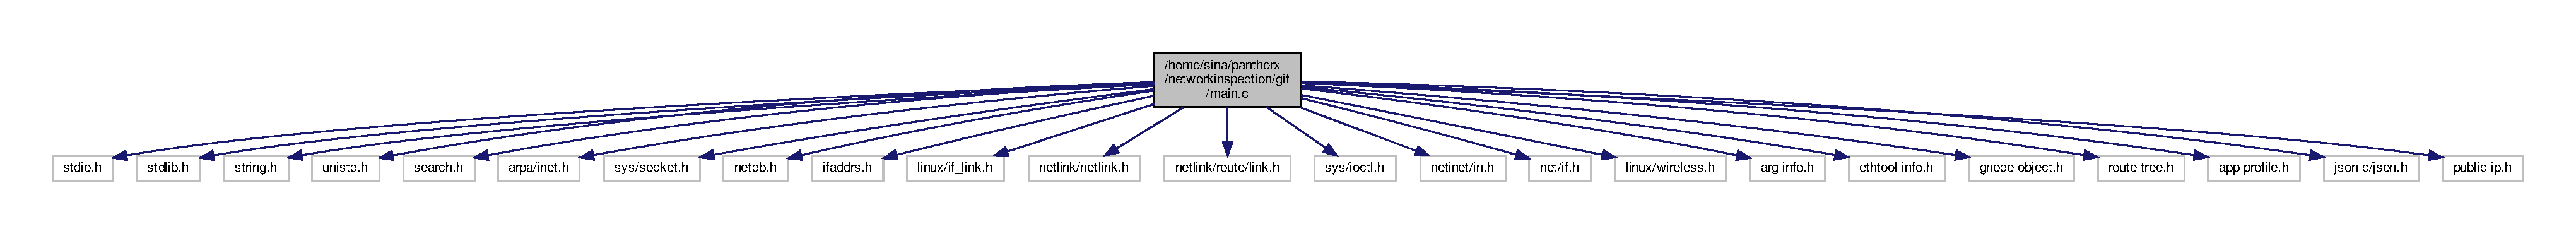
\includegraphics[width=350pt]{main_8c__incl}
\end{center}
\end{figure}
\subsection*{Enumerations}
\begin{DoxyCompactItemize}
\item 
enum \hyperlink{main_8c_a7bc1c477dae83ef66bdbd360fce8b3b7}{I\+F\+\_\+\+T\+R\+A\+V\+E\+R\+S\+E\+\_\+\+M\+O\+DE} \{ \hyperlink{main_8c_a7bc1c477dae83ef66bdbd360fce8b3b7a447898b405796e8408d14997383cd7f0}{P\+HY}, 
\hyperlink{main_8c_a7bc1c477dae83ef66bdbd360fce8b3b7a75039ed322737bab50d3a284f7bfc381}{T\+AP}, 
\hyperlink{main_8c_a7bc1c477dae83ef66bdbd360fce8b3b7a5a4e4e444e81403d9166b0fa64196761}{T\+UN}, 
\hyperlink{main_8c_a7bc1c477dae83ef66bdbd360fce8b3b7a309fd8ba753197f13b23ede644b0d58c}{P\+UB}
 \}\begin{DoxyCompactList}\small\item\em The traverse mode used for traversing group of interfaces. \end{DoxyCompactList}
\item 
enum \hyperlink{main_8c_a5ffcda19913c05c9d113f32fcd11805c}{I\+F\+\_\+\+M\+O\+DE} \{ \hyperlink{main_8c_a5ffcda19913c05c9d113f32fcd11805ca885cef154adf6c48c3392f8ca8898d75}{P\+H\+Y\+\_\+\+M\+O\+DE}, 
\hyperlink{main_8c_a5ffcda19913c05c9d113f32fcd11805ca17b28ff1a59054d22c2d4bf08eb638f0}{T\+A\+P\+\_\+\+M\+O\+DE}, 
\hyperlink{main_8c_a5ffcda19913c05c9d113f32fcd11805caac481b78320c3a986f8f81c29f86ef49}{T\+U\+N\+\_\+\+M\+O\+DE}, 
\hyperlink{main_8c_a5ffcda19913c05c9d113f32fcd11805ca46dbf2e0f925aa7b0f3f9edd25acf5e6}{I\+F\+\_\+\+N\+O\+NE}
 \}\begin{DoxyCompactList}\small\item\em The interface mode used to retrieve public IP. \end{DoxyCompactList}
\end{DoxyCompactItemize}
\subsection*{Functions}
\begin{DoxyCompactItemize}
\item 
void \hyperlink{main_8c_a345bf2d3cf0cd82bcbbba3e054eafd48}{find\+\_\+primary\+\_\+if\+\_\+index} ()
\begin{DoxyCompactList}\small\item\em Finds the primary interface. \end{DoxyCompactList}\item 
int \hyperlink{main_8c_ae6c1cdef3918f1d4c01e4c3c566bb211}{get\+\_\+wifi\+\_\+info} (const char $\ast$ifname, char $\ast$protocol, char $\ast$essid\+\_\+name)
\begin{DoxyCompactList}\small\item\em The function get one interface information. \end{DoxyCompactList}\item 
void \hyperlink{main_8c_a6f5d8c51479e6196fb3d19e3538a46d0}{get\+\_\+if\+\_\+info} (struct ifaddrs $\ast$ifa, int family, enum \hyperlink{main_8c_a7bc1c477dae83ef66bdbd360fce8b3b7}{I\+F\+\_\+\+T\+R\+A\+V\+E\+R\+S\+E\+\_\+\+M\+O\+DE} tr\+\_\+mode)
\begin{DoxyCompactList}\small\item\em The function get one interface information. \end{DoxyCompactList}\item 
void \hyperlink{main_8c_a5e3d195dba2da8b65b35a85c7834dfa2}{traverse\+\_\+ifs} (struct ifaddrs $\ast$ifaddr, enum \hyperlink{main_8c_a7bc1c477dae83ef66bdbd360fce8b3b7}{I\+F\+\_\+\+T\+R\+A\+V\+E\+R\+S\+E\+\_\+\+M\+O\+DE} tr\+\_\+mode)
\begin{DoxyCompactList}\small\item\em The function traverses interfaces. \end{DoxyCompactList}\item 
void \hyperlink{main_8c_a9af8032bea78a008241c6a446021e90b}{public\+\_\+ip\+\_\+retrieve} ()
\begin{DoxyCompactList}\small\item\em The function retrieve all public I\+Ps. \end{DoxyCompactList}\item 
void \hyperlink{main_8c_a25501fb2b3310a216de1ece7fa86e233}{get\+\_\+routes} ()
\begin{DoxyCompactList}\small\item\em The main function detects all routes to public network (Internet). \end{DoxyCompactList}\item 
int \hyperlink{main_8c_a3c04138a5bfe5d72780bb7e82a18e627}{main} (int argc, char $\ast$$\ast$argv)
\begin{DoxyCompactList}\small\item\em The main function of the project. \end{DoxyCompactList}\end{DoxyCompactItemize}


\subsection{Enumeration Type Documentation}
\mbox{\Hypertarget{main_8c_a5ffcda19913c05c9d113f32fcd11805c}\label{main_8c_a5ffcda19913c05c9d113f32fcd11805c}} 
\index{main.\+c@{main.\+c}!I\+F\+\_\+\+M\+O\+DE@{I\+F\+\_\+\+M\+O\+DE}}
\index{I\+F\+\_\+\+M\+O\+DE@{I\+F\+\_\+\+M\+O\+DE}!main.\+c@{main.\+c}}
\subsubsection{\texorpdfstring{I\+F\+\_\+\+M\+O\+DE}{IF\_MODE}}
{\footnotesize\ttfamily enum \hyperlink{main_8c_a5ffcda19913c05c9d113f32fcd11805c}{I\+F\+\_\+\+M\+O\+DE}}



The interface mode used to retrieve public IP. 

\begin{DoxyEnumFields}{Enumerator}
\raisebox{\heightof{T}}[0pt][0pt]{\index{P\+H\+Y\+\_\+\+M\+O\+DE@{P\+H\+Y\+\_\+\+M\+O\+DE}!main.\+c@{main.\+c}}\index{main.\+c@{main.\+c}!P\+H\+Y\+\_\+\+M\+O\+DE@{P\+H\+Y\+\_\+\+M\+O\+DE}}}\mbox{\Hypertarget{main_8c_a5ffcda19913c05c9d113f32fcd11805ca885cef154adf6c48c3392f8ca8898d75}\label{main_8c_a5ffcda19913c05c9d113f32fcd11805ca885cef154adf6c48c3392f8ca8898d75}} 
P\+H\+Y\+\_\+\+M\+O\+DE&The public IP is accessible via physical interface. \\
\hline

\raisebox{\heightof{T}}[0pt][0pt]{\index{T\+A\+P\+\_\+\+M\+O\+DE@{T\+A\+P\+\_\+\+M\+O\+DE}!main.\+c@{main.\+c}}\index{main.\+c@{main.\+c}!T\+A\+P\+\_\+\+M\+O\+DE@{T\+A\+P\+\_\+\+M\+O\+DE}}}\mbox{\Hypertarget{main_8c_a5ffcda19913c05c9d113f32fcd11805ca17b28ff1a59054d22c2d4bf08eb638f0}\label{main_8c_a5ffcda19913c05c9d113f32fcd11805ca17b28ff1a59054d22c2d4bf08eb638f0}} 
T\+A\+P\+\_\+\+M\+O\+DE&The public IP is accessible via tap interface. \\
\hline

\raisebox{\heightof{T}}[0pt][0pt]{\index{T\+U\+N\+\_\+\+M\+O\+DE@{T\+U\+N\+\_\+\+M\+O\+DE}!main.\+c@{main.\+c}}\index{main.\+c@{main.\+c}!T\+U\+N\+\_\+\+M\+O\+DE@{T\+U\+N\+\_\+\+M\+O\+DE}}}\mbox{\Hypertarget{main_8c_a5ffcda19913c05c9d113f32fcd11805caac481b78320c3a986f8f81c29f86ef49}\label{main_8c_a5ffcda19913c05c9d113f32fcd11805caac481b78320c3a986f8f81c29f86ef49}} 
T\+U\+N\+\_\+\+M\+O\+DE&The public IP is accessible via tun interface. \\
\hline

\raisebox{\heightof{T}}[0pt][0pt]{\index{I\+F\+\_\+\+N\+O\+NE@{I\+F\+\_\+\+N\+O\+NE}!main.\+c@{main.\+c}}\index{main.\+c@{main.\+c}!I\+F\+\_\+\+N\+O\+NE@{I\+F\+\_\+\+N\+O\+NE}}}\mbox{\Hypertarget{main_8c_a5ffcda19913c05c9d113f32fcd11805ca46dbf2e0f925aa7b0f3f9edd25acf5e6}\label{main_8c_a5ffcda19913c05c9d113f32fcd11805ca46dbf2e0f925aa7b0f3f9edd25acf5e6}} 
I\+F\+\_\+\+N\+O\+NE&The public IP is accessibility is not determined. \\
\hline

\end{DoxyEnumFields}
\mbox{\Hypertarget{main_8c_a7bc1c477dae83ef66bdbd360fce8b3b7}\label{main_8c_a7bc1c477dae83ef66bdbd360fce8b3b7}} 
\index{main.\+c@{main.\+c}!I\+F\+\_\+\+T\+R\+A\+V\+E\+R\+S\+E\+\_\+\+M\+O\+DE@{I\+F\+\_\+\+T\+R\+A\+V\+E\+R\+S\+E\+\_\+\+M\+O\+DE}}
\index{I\+F\+\_\+\+T\+R\+A\+V\+E\+R\+S\+E\+\_\+\+M\+O\+DE@{I\+F\+\_\+\+T\+R\+A\+V\+E\+R\+S\+E\+\_\+\+M\+O\+DE}!main.\+c@{main.\+c}}
\subsubsection{\texorpdfstring{I\+F\+\_\+\+T\+R\+A\+V\+E\+R\+S\+E\+\_\+\+M\+O\+DE}{IF\_TRAVERSE\_MODE}}
{\footnotesize\ttfamily enum \hyperlink{main_8c_a7bc1c477dae83ef66bdbd360fce8b3b7}{I\+F\+\_\+\+T\+R\+A\+V\+E\+R\+S\+E\+\_\+\+M\+O\+DE}}



The traverse mode used for traversing group of interfaces. 

\begin{DoxyEnumFields}{Enumerator}
\raisebox{\heightof{T}}[0pt][0pt]{\index{P\+HY@{P\+HY}!main.\+c@{main.\+c}}\index{main.\+c@{main.\+c}!P\+HY@{P\+HY}}}\mbox{\Hypertarget{main_8c_a7bc1c477dae83ef66bdbd360fce8b3b7a447898b405796e8408d14997383cd7f0}\label{main_8c_a7bc1c477dae83ef66bdbd360fce8b3b7a447898b405796e8408d14997383cd7f0}} 
P\+HY&Means physical interface. \\
\hline

\raisebox{\heightof{T}}[0pt][0pt]{\index{T\+AP@{T\+AP}!main.\+c@{main.\+c}}\index{main.\+c@{main.\+c}!T\+AP@{T\+AP}}}\mbox{\Hypertarget{main_8c_a7bc1c477dae83ef66bdbd360fce8b3b7a75039ed322737bab50d3a284f7bfc381}\label{main_8c_a7bc1c477dae83ef66bdbd360fce8b3b7a75039ed322737bab50d3a284f7bfc381}} 
T\+AP&Means tap-\/based interfaces. \\
\hline

\raisebox{\heightof{T}}[0pt][0pt]{\index{T\+UN@{T\+UN}!main.\+c@{main.\+c}}\index{main.\+c@{main.\+c}!T\+UN@{T\+UN}}}\mbox{\Hypertarget{main_8c_a7bc1c477dae83ef66bdbd360fce8b3b7a5a4e4e444e81403d9166b0fa64196761}\label{main_8c_a7bc1c477dae83ef66bdbd360fce8b3b7a5a4e4e444e81403d9166b0fa64196761}} 
T\+UN&Means tun-\/based interfaces. \\
\hline

\raisebox{\heightof{T}}[0pt][0pt]{\index{P\+UB@{P\+UB}!main.\+c@{main.\+c}}\index{main.\+c@{main.\+c}!P\+UB@{P\+UB}}}\mbox{\Hypertarget{main_8c_a7bc1c477dae83ef66bdbd360fce8b3b7a309fd8ba753197f13b23ede644b0d58c}\label{main_8c_a7bc1c477dae83ef66bdbd360fce8b3b7a309fd8ba753197f13b23ede644b0d58c}} 
P\+UB&Means public interfaces. Not used now. \\
\hline

\end{DoxyEnumFields}


\subsection{Function Documentation}
\mbox{\Hypertarget{main_8c_a345bf2d3cf0cd82bcbbba3e054eafd48}\label{main_8c_a345bf2d3cf0cd82bcbbba3e054eafd48}} 
\index{main.\+c@{main.\+c}!find\+\_\+primary\+\_\+if\+\_\+index@{find\+\_\+primary\+\_\+if\+\_\+index}}
\index{find\+\_\+primary\+\_\+if\+\_\+index@{find\+\_\+primary\+\_\+if\+\_\+index}!main.\+c@{main.\+c}}
\subsubsection{\texorpdfstring{find\+\_\+primary\+\_\+if\+\_\+index()}{find\_primary\_if\_index()}}
{\footnotesize\ttfamily void find\+\_\+primary\+\_\+if\+\_\+index (\begin{DoxyParamCaption}{ }\end{DoxyParamCaption})}



Finds the primary interface. 

The function finds the primary physical interface through which, the main traffic of the machine goes.

\begin{DoxySeeAlso}{See also}
\href{https://wiki.pantherx.org}{\tt https\+://wiki.\+pantherx.\+org} 
\end{DoxySeeAlso}
\begin{DoxyRefDesc}{Todo}
\item[\hyperlink{todo__todo000003}{Todo}]T\+O\+DO Support tap-\/based interfaces.\end{DoxyRefDesc}


\begin{DoxyPrecond}{Precondition}
The gstatic global variable kernel\+\_\+route\+\_\+roots must be set. 
\end{DoxyPrecond}
\begin{DoxyNote}{Note}
It sets the static global variable primary\+\_\+if\+\_\+index that indicates the index of primary physical interface. 
\end{DoxyNote}
\mbox{\Hypertarget{main_8c_a6f5d8c51479e6196fb3d19e3538a46d0}\label{main_8c_a6f5d8c51479e6196fb3d19e3538a46d0}} 
\index{main.\+c@{main.\+c}!get\+\_\+if\+\_\+info@{get\+\_\+if\+\_\+info}}
\index{get\+\_\+if\+\_\+info@{get\+\_\+if\+\_\+info}!main.\+c@{main.\+c}}
\subsubsection{\texorpdfstring{get\+\_\+if\+\_\+info()}{get\_if\_info()}}
{\footnotesize\ttfamily void get\+\_\+if\+\_\+info (\begin{DoxyParamCaption}\item[{struct ifaddrs $\ast$}]{ifa,  }\item[{int}]{family,  }\item[{enum \hyperlink{main_8c_a7bc1c477dae83ef66bdbd360fce8b3b7}{I\+F\+\_\+\+T\+R\+A\+V\+E\+R\+S\+E\+\_\+\+M\+O\+DE}}]{tr\+\_\+mode }\end{DoxyParamCaption})}



The function get one interface information. 

The function uses many different A\+PI and libraries to gather interfaces information.

\begin{DoxySeeAlso}{See also}
\href{https://wiki.pantherx.org}{\tt https\+://wiki.\+pantherx.\+org} 
\end{DoxySeeAlso}
\begin{DoxyRefDesc}{Todo}
\item[\hyperlink{todo__todo000004}{Todo}]T\+O\+DO Support tap-\/based interfaces.\end{DoxyRefDesc}


\begin{DoxyPrecond}{Precondition}
The input must be provided. The kernel\+\_\+route\+\_\+roots must be set. The V\+PN type and profile must be detected. 
\end{DoxyPrecond}

\begin{DoxyParams}[1]{Parameters}
\mbox{\tt in}  & {\em ifa} & The input network interface. \\
\hline
\mbox{\tt in}  & {\em family} & The protocol family of the interface (i.\+e inet or inet6). \\
\hline
\mbox{\tt in}  & {\em tr\+\_\+mode} & The type of interfaces to be traversed. \\
\hline
\end{DoxyParams}
\begin{DoxyNote}{Note}
It uses kernel\+\_\+route\+\_\+roots and affects other static global variables and arrays. 
\end{DoxyNote}
\mbox{\Hypertarget{main_8c_a25501fb2b3310a216de1ece7fa86e233}\label{main_8c_a25501fb2b3310a216de1ece7fa86e233}} 
\index{main.\+c@{main.\+c}!get\+\_\+routes@{get\+\_\+routes}}
\index{get\+\_\+routes@{get\+\_\+routes}!main.\+c@{main.\+c}}
\subsubsection{\texorpdfstring{get\+\_\+routes()}{get\_routes()}}
{\footnotesize\ttfamily void get\+\_\+routes (\begin{DoxyParamCaption}{ }\end{DoxyParamCaption})}



The main function detects all routes to public network (Internet). 

The main function traverse the route and interfaces trees to establish all routes.

\begin{DoxySeeAlso}{See also}
\href{https://wiki.pantherx.org}{\tt https\+://wiki.\+pantherx.\+org} 
\end{DoxySeeAlso}
\begin{DoxyRefDesc}{Todo}
\item[\hyperlink{todo__todo000007}{Todo}]T\+O\+DO Add complicated routes. T\+O\+DO Support tap-\/based V\+P\+Ns.\end{DoxyRefDesc}


\begin{DoxyPrecond}{Precondition}
It must be called after detect\+\_\+vpn\+\_\+method, get\+\_\+vpn\+\_\+profile\+\_\+name, argp\+\_\+parse, and analyze\+\_\+kernel\+\_\+route functions. 
\end{DoxyPrecond}
\begin{DoxyPostcond}{Postcondition}
The detected routes have to be traversed to produce J\+S\+ON output. 
\end{DoxyPostcond}
\mbox{\Hypertarget{main_8c_ae6c1cdef3918f1d4c01e4c3c566bb211}\label{main_8c_ae6c1cdef3918f1d4c01e4c3c566bb211}} 
\index{main.\+c@{main.\+c}!get\+\_\+wifi\+\_\+info@{get\+\_\+wifi\+\_\+info}}
\index{get\+\_\+wifi\+\_\+info@{get\+\_\+wifi\+\_\+info}!main.\+c@{main.\+c}}
\subsubsection{\texorpdfstring{get\+\_\+wifi\+\_\+info()}{get\_wifi\_info()}}
{\footnotesize\ttfamily int get\+\_\+wifi\+\_\+info (\begin{DoxyParamCaption}\item[{const char $\ast$}]{ifname,  }\item[{char $\ast$}]{protocol,  }\item[{char $\ast$}]{essid\+\_\+name }\end{DoxyParamCaption})}



The function get one interface information. 

The function uses many different A\+PI and libraries to gather interfaces information.

\begin{DoxySeeAlso}{See also}
\href{https://wiki.pantherx.org}{\tt https\+://wiki.\+pantherx.\+org}
\end{DoxySeeAlso}

\begin{DoxyParams}[1]{Parameters}
\mbox{\tt in}  & {\em ifname} & The input network interface to be checked for wifi information. \\
\hline
\mbox{\tt out}  & {\em protocol} & The running link-\/layer protocol of wifi (e.\+g I\+E\+EE 802.\+a). \\
\hline
\mbox{\tt out}  & {\em essid\+\_\+name} & The name of the access point that the wifi interface is connected to. \\
\hline
\end{DoxyParams}
\begin{DoxyNote}{Note}
It uses kernel\textquotesingle{}s wifi interface. 
\end{DoxyNote}
\mbox{\Hypertarget{main_8c_a3c04138a5bfe5d72780bb7e82a18e627}\label{main_8c_a3c04138a5bfe5d72780bb7e82a18e627}} 
\index{main.\+c@{main.\+c}!main@{main}}
\index{main@{main}!main.\+c@{main.\+c}}
\subsubsection{\texorpdfstring{main()}{main()}}
{\footnotesize\ttfamily int main (\begin{DoxyParamCaption}\item[{int}]{argc,  }\item[{char $\ast$$\ast$}]{argv }\end{DoxyParamCaption})}



The main function of the project. 

\begin{DoxyAuthor}{Author}
Sina Mahmoodi
\end{DoxyAuthor}
The main get input arguments, uses the vpn detection, public IP detection, route parsing, and network interface to inspect the network.

\begin{DoxySeeAlso}{See also}
\href{https://wiki.pantherx.org}{\tt https\+://wiki.\+pantherx.\+org}
\end{DoxySeeAlso}
\begin{DoxyRemark}{Remarks}
px-\/network-\/inspection provides J\+S\+ON based output in both file and stdout. Use px-\/network-\/inspection --usage to see the command help. 
\end{DoxyRemark}
\mbox{\Hypertarget{main_8c_a9af8032bea78a008241c6a446021e90b}\label{main_8c_a9af8032bea78a008241c6a446021e90b}} 
\index{main.\+c@{main.\+c}!public\+\_\+ip\+\_\+retrieve@{public\+\_\+ip\+\_\+retrieve}}
\index{public\+\_\+ip\+\_\+retrieve@{public\+\_\+ip\+\_\+retrieve}!main.\+c@{main.\+c}}
\subsubsection{\texorpdfstring{public\+\_\+ip\+\_\+retrieve()}{public\_ip\_retrieve()}}
{\footnotesize\ttfamily void public\+\_\+ip\+\_\+retrieve (\begin{DoxyParamCaption}{ }\end{DoxyParamCaption})}



The function retrieve all public I\+Ps. 

The main function gets publlic I\+Ps based on the V\+PN model.

\begin{DoxySeeAlso}{See also}
\href{https://wiki.pantherx.org}{\tt https\+://wiki.\+pantherx.\+org} 
\end{DoxySeeAlso}
\begin{DoxyRefDesc}{Todo}
\item[\hyperlink{todo__todo000006}{Todo}]T\+O\+DO Support tap-\/based V\+P\+Ns.\end{DoxyRefDesc}


\begin{DoxyPrecond}{Precondition}
All routes must be extracted. 
\end{DoxyPrecond}
\mbox{\Hypertarget{main_8c_a5e3d195dba2da8b65b35a85c7834dfa2}\label{main_8c_a5e3d195dba2da8b65b35a85c7834dfa2}} 
\index{main.\+c@{main.\+c}!traverse\+\_\+ifs@{traverse\+\_\+ifs}}
\index{traverse\+\_\+ifs@{traverse\+\_\+ifs}!main.\+c@{main.\+c}}
\subsubsection{\texorpdfstring{traverse\+\_\+ifs()}{traverse\_ifs()}}
{\footnotesize\ttfamily void traverse\+\_\+ifs (\begin{DoxyParamCaption}\item[{struct ifaddrs $\ast$}]{ifaddr,  }\item[{enum \hyperlink{main_8c_a7bc1c477dae83ef66bdbd360fce8b3b7}{I\+F\+\_\+\+T\+R\+A\+V\+E\+R\+S\+E\+\_\+\+M\+O\+DE}}]{tr\+\_\+mode }\end{DoxyParamCaption})}



The function traverses interfaces. 

The function traverses a group network interfaces according to their device type\+: P\+HY, T\+UN, T\+AP, and ....

\begin{DoxySeeAlso}{See also}
\href{https://wiki.pantherx.org}{\tt https\+://wiki.\+pantherx.\+org} 
\end{DoxySeeAlso}
\begin{DoxyRefDesc}{Todo}
\item[\hyperlink{todo__todo000005}{Todo}]T\+O\+DO Support tap-\/based interfaces.\end{DoxyRefDesc}


\begin{DoxyPrecond}{Precondition}
The input must be provided. 
\end{DoxyPrecond}

\begin{DoxyParams}[1]{Parameters}
\mbox{\tt in}  & {\em ifaddr} & List of input network interfaces to be checked and traversed. \\
\hline
\mbox{\tt in}  & {\em tr\+\_\+mode} & The type of interfaces to be traversed. \\
\hline
\end{DoxyParams}
\begin{DoxyNote}{Note}
It uses kernel\+\_\+route\+\_\+roots and affects other static global variables and arrays. 
\end{DoxyNote}

\hypertarget{public-ip_8c}{}\section{/home/sina/pantherx/networkinspection/git/public-\/ip.c File Reference}
\label{public-ip_8c}\index{/home/sina/pantherx/networkinspection/git/public-\/ip.\+c@{/home/sina/pantherx/networkinspection/git/public-\/ip.\+c}}
{\ttfamily \#include $<$public-\/ip.\+h$>$}\newline
{\ttfamily \#include $<$stdio.\+h$>$}\newline
{\ttfamily \#include $<$stdlib.\+h$>$}\newline
{\ttfamily \#include $<$string.\+h$>$}\newline
{\ttfamily \#include $<$curl/curl.\+h$>$}\newline
Include dependency graph for public-\/ip.c\+:\nopagebreak
\begin{figure}[H]
\begin{center}
\leavevmode
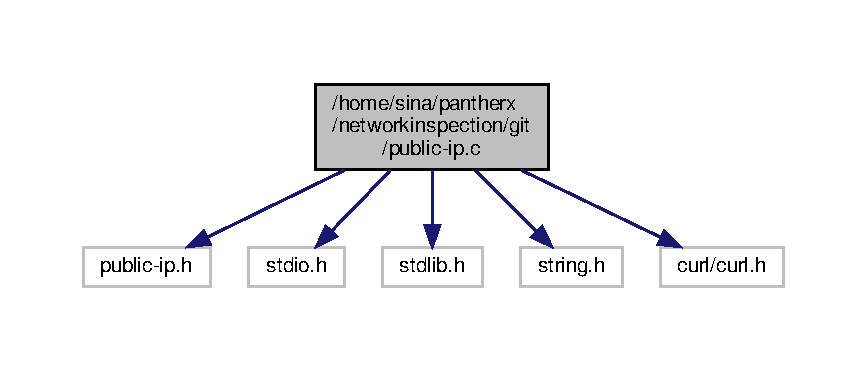
\includegraphics[width=350pt]{public-ip_8c__incl}
\end{center}
\end{figure}
\subsection*{Functions}
\begin{DoxyCompactItemize}
\item 
struct \hyperlink{structurl__data}{url\+\_\+data} $\ast$ \hyperlink{public-ip_8c_a546e9ee82a2fff0c37e173d76ab08db4}{handle\+\_\+url} (char $\ast$url, char $\ast$if\+\_\+name)
\item 
void \hyperlink{public-ip_8c_a343631cf6f2ceb1736d8b227c2cf76d3}{get\+\_\+public\+\_\+ip} (char if\+\_\+names\mbox{[}\hyperlink{route-tree_8h_a5f66955385e84e67789d731b5cad24c7}{M\+A\+X\+\_\+\+P\+H\+Y\+S\+\_\+\+I\+FS}\mbox{]}\mbox{[}16\mbox{]}, int if\+\_\+number, char if\+\_\+public\+\_\+ips\mbox{[}\hyperlink{route-tree_8h_a5f66955385e84e67789d731b5cad24c7}{M\+A\+X\+\_\+\+P\+H\+Y\+S\+\_\+\+I\+FS}\mbox{]}\mbox{[}40\mbox{]})
\end{DoxyCompactItemize}


\subsection{Function Documentation}
\mbox{\Hypertarget{public-ip_8c_a343631cf6f2ceb1736d8b227c2cf76d3}\label{public-ip_8c_a343631cf6f2ceb1736d8b227c2cf76d3}} 
\index{public-\/ip.\+c@{public-\/ip.\+c}!get\+\_\+public\+\_\+ip@{get\+\_\+public\+\_\+ip}}
\index{get\+\_\+public\+\_\+ip@{get\+\_\+public\+\_\+ip}!public-\/ip.\+c@{public-\/ip.\+c}}
\subsubsection{\texorpdfstring{get\+\_\+public\+\_\+ip()}{get\_public\_ip()}}
{\footnotesize\ttfamily void get\+\_\+public\+\_\+ip (\begin{DoxyParamCaption}\item[{char}]{if\+\_\+names\mbox{[}\+M\+A\+X\+\_\+\+P\+H\+Y\+S\+\_\+\+I\+F\+S\mbox{]}\mbox{[}16\mbox{]},  }\item[{int}]{if\+\_\+number,  }\item[{char}]{if\+\_\+public\+\_\+ips\mbox{[}\+M\+A\+X\+\_\+\+P\+H\+Y\+S\+\_\+\+I\+F\+S\mbox{]}\mbox{[}40\mbox{]} }\end{DoxyParamCaption})}

\mbox{\Hypertarget{public-ip_8c_a546e9ee82a2fff0c37e173d76ab08db4}\label{public-ip_8c_a546e9ee82a2fff0c37e173d76ab08db4}} 
\index{public-\/ip.\+c@{public-\/ip.\+c}!handle\+\_\+url@{handle\+\_\+url}}
\index{handle\+\_\+url@{handle\+\_\+url}!public-\/ip.\+c@{public-\/ip.\+c}}
\subsubsection{\texorpdfstring{handle\+\_\+url()}{handle\_url()}}
{\footnotesize\ttfamily struct \hyperlink{structurl__data}{url\+\_\+data}$\ast$ handle\+\_\+url (\begin{DoxyParamCaption}\item[{char $\ast$}]{url,  }\item[{char $\ast$}]{if\+\_\+name }\end{DoxyParamCaption})}


\hypertarget{README_8md}{}\section{/home/sina/pantherx/networkinspection/git/\+R\+E\+A\+D\+ME.md File Reference}
\label{README_8md}\index{/home/sina/pantherx/networkinspection/git/\+R\+E\+A\+D\+M\+E.\+md@{/home/sina/pantherx/networkinspection/git/\+R\+E\+A\+D\+M\+E.\+md}}

\hypertarget{route-tree_8c}{}\section{/home/sina/pantherx/networkinspection/git/route-\/tree.c File Reference}
\label{route-tree_8c}\index{/home/sina/pantherx/networkinspection/git/route-\/tree.\+c@{/home/sina/pantherx/networkinspection/git/route-\/tree.\+c}}
{\ttfamily \#include $<$route-\/tree.\+h$>$}\newline
{\ttfamily \#include $<$limits.\+h$>$}\newline
Include dependency graph for route-\/tree.c\+:\nopagebreak
\begin{figure}[H]
\begin{center}
\leavevmode
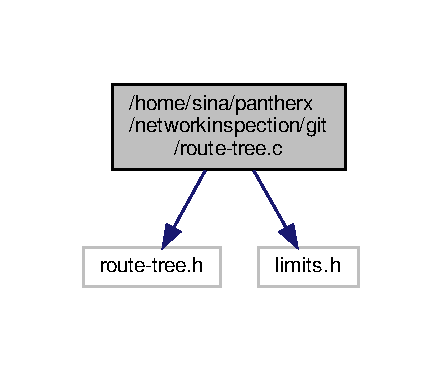
\includegraphics[width=350pt]{route-tree_8c__incl}
\end{center}
\end{figure}
\subsection*{Classes}
\begin{DoxyCompactItemize}
\item 
struct \hyperlink{structnode__params}{node\+\_\+params}
\item 
struct \hyperlink{structnode__search}{node\+\_\+search}
\end{DoxyCompactItemize}
\subsection*{Typedefs}
\begin{DoxyCompactItemize}
\item 
typedef struct \hyperlink{structnode__params}{node\+\_\+params} \hyperlink{route-tree_8c_a3aa763b62cd1d285ed35bb7f0fe4d149}{Node\+Params}
\item 
typedef struct \hyperlink{structnode__search}{node\+\_\+search} \hyperlink{route-tree_8c_a26d9b840f9226a0ce349b00950ea0bdc}{Node\+Search}
\end{DoxyCompactItemize}
\subsection*{Enumerations}
\begin{DoxyCompactItemize}
\item 
enum \hyperlink{route-tree_8c_aed8cdbb52dbe32c343a8c26887888e7f}{R\+O\+U\+T\+E\+\_\+\+Q\+U\+E\+RY} \{ \hyperlink{route-tree_8c_aed8cdbb52dbe32c343a8c26887888e7fab02d9a33d5a8476efc87ecc7049cc120}{R\+O\+U\+T\+E\+\_\+\+Q\+U\+E\+R\+Y\+\_\+\+G\+E\+T\+\_\+\+T\+R\+EE}, 
\hyperlink{route-tree_8c_aed8cdbb52dbe32c343a8c26887888e7fae1f920d24672bfd2b4deee446627d969}{R\+O\+U\+T\+E\+\_\+\+Q\+U\+E\+R\+Y\+\_\+\+G\+E\+T\+\_\+\+F\+I\+R\+ST}
 \}
\end{DoxyCompactItemize}
\subsection*{Functions}
\begin{DoxyCompactItemize}
\item 
\hyperlink{route-tree_8h_a1034dd038389279bf422489d4d99d43a}{Vpn\+Method} $\ast$ \hyperlink{route-tree_8c_a3ccbf1b413fe282c1490701f739273a8}{vpn\+\_\+method\+\_\+new} ()
\item 
void \hyperlink{route-tree_8c_a06257b65d43c86e35b44ae0d91b226cf}{vpn\+\_\+method\+\_\+free} ()
\item 
\hyperlink{route-tree_8h_a1296be44c6672a1adb94ba6dc416682c}{Route\+Node} $\ast$ \hyperlink{route-tree_8c_a941ed51572db1d1d4720f8a329dd0d8b}{route\+\_\+node\+\_\+new} ()
\item 
void \hyperlink{route-tree_8c_a1b80d492072ee18f906bdd2fbaad9b4b}{route\+\_\+node\+\_\+free} (\hyperlink{route-tree_8h_a1296be44c6672a1adb94ba6dc416682c}{Route\+Node} $\ast$nd)
\item 
void \hyperlink{route-tree_8c_ac750dd5c6890dd949d1029d4363fa0e0}{first\+\_\+entry\+\_\+cb} (struct nl\+\_\+object $\ast$obj, void $\ast$data)
\item 
void \hyperlink{route-tree_8c_a8402c2baca9819b3791b35b6c1645ce6}{next\+\_\+hop\+\_\+entry\+\_\+cb} (struct rtnl\+\_\+nexthop $\ast$nh, void $\ast$data)
\item 
void \hyperlink{route-tree_8c_a112b373b8e4a4a0eacfba3cc078e5ce2}{route\+\_\+entry\+\_\+cb} (struct nl\+\_\+object $\ast$obj, void $\ast$data)
\item 
void \hyperlink{route-tree_8c_a7e256826bca6c828a8564f27f84dd517}{get\+\_\+route\+\_\+trees} (enum \hyperlink{route-tree_8c_aed8cdbb52dbe32c343a8c26887888e7f}{R\+O\+U\+T\+E\+\_\+\+Q\+U\+E\+RY} query\+\_\+id, G\+Node $\ast$node\mbox{[}\hyperlink{route-tree_8h_a8e1da3af3417de420798c8b448b6a8cb}{M\+A\+X\+\_\+\+R\+O\+O\+T\+S\+\_\+\+N\+U\+M\+B\+ER}\mbox{]}, int $\ast$roots, int argc, char $\ast$argv\mbox{[}$\,$\mbox{]})
\item 
int \hyperlink{route-tree_8c_a023982baea4d991af1755c75365e6070}{analyze\+\_\+openvpn\+\_\+kernel\+\_\+route} (G\+Node $\ast$kernel\+\_\+route\+\_\+roots\mbox{[}\hyperlink{route-tree_8h_a8e1da3af3417de420798c8b448b6a8cb}{M\+A\+X\+\_\+\+R\+O\+O\+T\+S\+\_\+\+N\+U\+M\+B\+ER}\mbox{]}, int $\ast$kernel\+\_\+roots)
\item 
int \hyperlink{route-tree_8c_ad4fe4de0af6177aad9c1936fcaa1d988}{analyze\+\_\+anyconnect\+\_\+kernel\+\_\+route} (G\+Node $\ast$kernel\+\_\+route\+\_\+roots\mbox{[}\hyperlink{route-tree_8h_a8e1da3af3417de420798c8b448b6a8cb}{M\+A\+X\+\_\+\+R\+O\+O\+T\+S\+\_\+\+N\+U\+M\+B\+ER}\mbox{]}, int $\ast$kernel\+\_\+roots)
\item 
int \hyperlink{route-tree_8c_a5a490e2e29be18ae630572e3776539af}{analyze\+\_\+kernel\+\_\+route} (G\+Node $\ast$kernel\+\_\+route\+\_\+roots\mbox{[}\hyperlink{route-tree_8h_a8e1da3af3417de420798c8b448b6a8cb}{M\+A\+X\+\_\+\+R\+O\+O\+T\+S\+\_\+\+N\+U\+M\+B\+ER}\mbox{]}, int $\ast$kernel\+\_\+roots, enum \hyperlink{route-tree_8h_a5b876670828c4e38106ba1c6d91024b7}{V\+P\+N\+\_\+\+M\+E\+T\+H\+O\+DS} vpn\+\_\+method)
\item 
gboolean \hyperlink{route-tree_8c_a3a0eeaa4d6b227ed8aa19e5d56096cd3}{find\+\_\+node\+\_\+traverse} (G\+Node $\ast$node, gpointer data)
\item 
G\+Node $\ast$ \hyperlink{route-tree_8c_a77affcaa875961893c05c7e211678ed1}{get\+\_\+kernel\+\_\+route\+\_\+node} (G\+Node $\ast$kernel\+\_\+route\+\_\+roots\mbox{[}\hyperlink{route-tree_8h_a8e1da3af3417de420798c8b448b6a8cb}{M\+A\+X\+\_\+\+R\+O\+O\+T\+S\+\_\+\+N\+U\+M\+B\+ER}\mbox{]}, int roots, char $\ast$ifa\+\_\+name)
\item 
\hyperlink{route-tree_8h_a1034dd038389279bf422489d4d99d43a}{Vpn\+Method} $\ast$ \hyperlink{route-tree_8c_a267529614de44218b8187f3ac46ce46f}{detect\+\_\+vpn\+\_\+method} ()
\end{DoxyCompactItemize}


\subsection{Typedef Documentation}
\mbox{\Hypertarget{route-tree_8c_a3aa763b62cd1d285ed35bb7f0fe4d149}\label{route-tree_8c_a3aa763b62cd1d285ed35bb7f0fe4d149}} 
\index{route-\/tree.\+c@{route-\/tree.\+c}!Node\+Params@{Node\+Params}}
\index{Node\+Params@{Node\+Params}!route-\/tree.\+c@{route-\/tree.\+c}}
\subsubsection{\texorpdfstring{Node\+Params}{NodeParams}}
{\footnotesize\ttfamily typedef struct \hyperlink{structnode__params}{node\+\_\+params}  \hyperlink{route-tree_8c_a3aa763b62cd1d285ed35bb7f0fe4d149}{Node\+Params}}

\mbox{\Hypertarget{route-tree_8c_a26d9b840f9226a0ce349b00950ea0bdc}\label{route-tree_8c_a26d9b840f9226a0ce349b00950ea0bdc}} 
\index{route-\/tree.\+c@{route-\/tree.\+c}!Node\+Search@{Node\+Search}}
\index{Node\+Search@{Node\+Search}!route-\/tree.\+c@{route-\/tree.\+c}}
\subsubsection{\texorpdfstring{Node\+Search}{NodeSearch}}
{\footnotesize\ttfamily typedef struct \hyperlink{structnode__search}{node\+\_\+search}  \hyperlink{route-tree_8c_a26d9b840f9226a0ce349b00950ea0bdc}{Node\+Search}}



\subsection{Enumeration Type Documentation}
\mbox{\Hypertarget{route-tree_8c_aed8cdbb52dbe32c343a8c26887888e7f}\label{route-tree_8c_aed8cdbb52dbe32c343a8c26887888e7f}} 
\index{route-\/tree.\+c@{route-\/tree.\+c}!R\+O\+U\+T\+E\+\_\+\+Q\+U\+E\+RY@{R\+O\+U\+T\+E\+\_\+\+Q\+U\+E\+RY}}
\index{R\+O\+U\+T\+E\+\_\+\+Q\+U\+E\+RY@{R\+O\+U\+T\+E\+\_\+\+Q\+U\+E\+RY}!route-\/tree.\+c@{route-\/tree.\+c}}
\subsubsection{\texorpdfstring{R\+O\+U\+T\+E\+\_\+\+Q\+U\+E\+RY}{ROUTE\_QUERY}}
{\footnotesize\ttfamily enum \hyperlink{route-tree_8c_aed8cdbb52dbe32c343a8c26887888e7f}{R\+O\+U\+T\+E\+\_\+\+Q\+U\+E\+RY}}

\begin{DoxyEnumFields}{Enumerator}
\raisebox{\heightof{T}}[0pt][0pt]{\index{R\+O\+U\+T\+E\+\_\+\+Q\+U\+E\+R\+Y\+\_\+\+G\+E\+T\+\_\+\+T\+R\+EE@{R\+O\+U\+T\+E\+\_\+\+Q\+U\+E\+R\+Y\+\_\+\+G\+E\+T\+\_\+\+T\+R\+EE}!route-\/tree.\+c@{route-\/tree.\+c}}\index{route-\/tree.\+c@{route-\/tree.\+c}!R\+O\+U\+T\+E\+\_\+\+Q\+U\+E\+R\+Y\+\_\+\+G\+E\+T\+\_\+\+T\+R\+EE@{R\+O\+U\+T\+E\+\_\+\+Q\+U\+E\+R\+Y\+\_\+\+G\+E\+T\+\_\+\+T\+R\+EE}}}\mbox{\Hypertarget{route-tree_8c_aed8cdbb52dbe32c343a8c26887888e7fab02d9a33d5a8476efc87ecc7049cc120}\label{route-tree_8c_aed8cdbb52dbe32c343a8c26887888e7fab02d9a33d5a8476efc87ecc7049cc120}} 
R\+O\+U\+T\+E\+\_\+\+Q\+U\+E\+R\+Y\+\_\+\+G\+E\+T\+\_\+\+T\+R\+EE&\\
\hline

\raisebox{\heightof{T}}[0pt][0pt]{\index{R\+O\+U\+T\+E\+\_\+\+Q\+U\+E\+R\+Y\+\_\+\+G\+E\+T\+\_\+\+F\+I\+R\+ST@{R\+O\+U\+T\+E\+\_\+\+Q\+U\+E\+R\+Y\+\_\+\+G\+E\+T\+\_\+\+F\+I\+R\+ST}!route-\/tree.\+c@{route-\/tree.\+c}}\index{route-\/tree.\+c@{route-\/tree.\+c}!R\+O\+U\+T\+E\+\_\+\+Q\+U\+E\+R\+Y\+\_\+\+G\+E\+T\+\_\+\+F\+I\+R\+ST@{R\+O\+U\+T\+E\+\_\+\+Q\+U\+E\+R\+Y\+\_\+\+G\+E\+T\+\_\+\+F\+I\+R\+ST}}}\mbox{\Hypertarget{route-tree_8c_aed8cdbb52dbe32c343a8c26887888e7fae1f920d24672bfd2b4deee446627d969}\label{route-tree_8c_aed8cdbb52dbe32c343a8c26887888e7fae1f920d24672bfd2b4deee446627d969}} 
R\+O\+U\+T\+E\+\_\+\+Q\+U\+E\+R\+Y\+\_\+\+G\+E\+T\+\_\+\+F\+I\+R\+ST&\\
\hline

\end{DoxyEnumFields}


\subsection{Function Documentation}
\mbox{\Hypertarget{route-tree_8c_ad4fe4de0af6177aad9c1936fcaa1d988}\label{route-tree_8c_ad4fe4de0af6177aad9c1936fcaa1d988}} 
\index{route-\/tree.\+c@{route-\/tree.\+c}!analyze\+\_\+anyconnect\+\_\+kernel\+\_\+route@{analyze\+\_\+anyconnect\+\_\+kernel\+\_\+route}}
\index{analyze\+\_\+anyconnect\+\_\+kernel\+\_\+route@{analyze\+\_\+anyconnect\+\_\+kernel\+\_\+route}!route-\/tree.\+c@{route-\/tree.\+c}}
\subsubsection{\texorpdfstring{analyze\+\_\+anyconnect\+\_\+kernel\+\_\+route()}{analyze\_anyconnect\_kernel\_route()}}
{\footnotesize\ttfamily int analyze\+\_\+anyconnect\+\_\+kernel\+\_\+route (\begin{DoxyParamCaption}\item[{G\+Node $\ast$}]{kernel\+\_\+route\+\_\+roots\mbox{[}\+M\+A\+X\+\_\+\+R\+O\+O\+T\+S\+\_\+\+N\+U\+M\+B\+E\+R\mbox{]},  }\item[{int $\ast$}]{kernel\+\_\+roots }\end{DoxyParamCaption})}

\mbox{\Hypertarget{route-tree_8c_a5a490e2e29be18ae630572e3776539af}\label{route-tree_8c_a5a490e2e29be18ae630572e3776539af}} 
\index{route-\/tree.\+c@{route-\/tree.\+c}!analyze\+\_\+kernel\+\_\+route@{analyze\+\_\+kernel\+\_\+route}}
\index{analyze\+\_\+kernel\+\_\+route@{analyze\+\_\+kernel\+\_\+route}!route-\/tree.\+c@{route-\/tree.\+c}}
\subsubsection{\texorpdfstring{analyze\+\_\+kernel\+\_\+route()}{analyze\_kernel\_route()}}
{\footnotesize\ttfamily int analyze\+\_\+kernel\+\_\+route (\begin{DoxyParamCaption}\item[{G\+Node $\ast$}]{kernel\+\_\+route\+\_\+roots\mbox{[}\+M\+A\+X\+\_\+\+R\+O\+O\+T\+S\+\_\+\+N\+U\+M\+B\+E\+R\mbox{]},  }\item[{int $\ast$}]{kernel\+\_\+roots,  }\item[{enum \hyperlink{route-tree_8h_a5b876670828c4e38106ba1c6d91024b7}{V\+P\+N\+\_\+\+M\+E\+T\+H\+O\+DS}}]{vpn\+\_\+method }\end{DoxyParamCaption})}

\mbox{\Hypertarget{route-tree_8c_a023982baea4d991af1755c75365e6070}\label{route-tree_8c_a023982baea4d991af1755c75365e6070}} 
\index{route-\/tree.\+c@{route-\/tree.\+c}!analyze\+\_\+openvpn\+\_\+kernel\+\_\+route@{analyze\+\_\+openvpn\+\_\+kernel\+\_\+route}}
\index{analyze\+\_\+openvpn\+\_\+kernel\+\_\+route@{analyze\+\_\+openvpn\+\_\+kernel\+\_\+route}!route-\/tree.\+c@{route-\/tree.\+c}}
\subsubsection{\texorpdfstring{analyze\+\_\+openvpn\+\_\+kernel\+\_\+route()}{analyze\_openvpn\_kernel\_route()}}
{\footnotesize\ttfamily int analyze\+\_\+openvpn\+\_\+kernel\+\_\+route (\begin{DoxyParamCaption}\item[{G\+Node $\ast$}]{kernel\+\_\+route\+\_\+roots\mbox{[}\+M\+A\+X\+\_\+\+R\+O\+O\+T\+S\+\_\+\+N\+U\+M\+B\+E\+R\mbox{]},  }\item[{int $\ast$}]{kernel\+\_\+roots }\end{DoxyParamCaption})}

\mbox{\Hypertarget{route-tree_8c_a267529614de44218b8187f3ac46ce46f}\label{route-tree_8c_a267529614de44218b8187f3ac46ce46f}} 
\index{route-\/tree.\+c@{route-\/tree.\+c}!detect\+\_\+vpn\+\_\+method@{detect\+\_\+vpn\+\_\+method}}
\index{detect\+\_\+vpn\+\_\+method@{detect\+\_\+vpn\+\_\+method}!route-\/tree.\+c@{route-\/tree.\+c}}
\subsubsection{\texorpdfstring{detect\+\_\+vpn\+\_\+method()}{detect\_vpn\_method()}}
{\footnotesize\ttfamily \hyperlink{route-tree_8h_a1034dd038389279bf422489d4d99d43a}{Vpn\+Method}$\ast$ detect\+\_\+vpn\+\_\+method (\begin{DoxyParamCaption}{ }\end{DoxyParamCaption})}

\mbox{\Hypertarget{route-tree_8c_a3a0eeaa4d6b227ed8aa19e5d56096cd3}\label{route-tree_8c_a3a0eeaa4d6b227ed8aa19e5d56096cd3}} 
\index{route-\/tree.\+c@{route-\/tree.\+c}!find\+\_\+node\+\_\+traverse@{find\+\_\+node\+\_\+traverse}}
\index{find\+\_\+node\+\_\+traverse@{find\+\_\+node\+\_\+traverse}!route-\/tree.\+c@{route-\/tree.\+c}}
\subsubsection{\texorpdfstring{find\+\_\+node\+\_\+traverse()}{find\_node\_traverse()}}
{\footnotesize\ttfamily gboolean find\+\_\+node\+\_\+traverse (\begin{DoxyParamCaption}\item[{G\+Node $\ast$}]{node,  }\item[{gpointer}]{data }\end{DoxyParamCaption})}

\mbox{\Hypertarget{route-tree_8c_ac750dd5c6890dd949d1029d4363fa0e0}\label{route-tree_8c_ac750dd5c6890dd949d1029d4363fa0e0}} 
\index{route-\/tree.\+c@{route-\/tree.\+c}!first\+\_\+entry\+\_\+cb@{first\+\_\+entry\+\_\+cb}}
\index{first\+\_\+entry\+\_\+cb@{first\+\_\+entry\+\_\+cb}!route-\/tree.\+c@{route-\/tree.\+c}}
\subsubsection{\texorpdfstring{first\+\_\+entry\+\_\+cb()}{first\_entry\_cb()}}
{\footnotesize\ttfamily void first\+\_\+entry\+\_\+cb (\begin{DoxyParamCaption}\item[{struct nl\+\_\+object $\ast$}]{obj,  }\item[{void $\ast$}]{data }\end{DoxyParamCaption})}

\mbox{\Hypertarget{route-tree_8c_a77affcaa875961893c05c7e211678ed1}\label{route-tree_8c_a77affcaa875961893c05c7e211678ed1}} 
\index{route-\/tree.\+c@{route-\/tree.\+c}!get\+\_\+kernel\+\_\+route\+\_\+node@{get\+\_\+kernel\+\_\+route\+\_\+node}}
\index{get\+\_\+kernel\+\_\+route\+\_\+node@{get\+\_\+kernel\+\_\+route\+\_\+node}!route-\/tree.\+c@{route-\/tree.\+c}}
\subsubsection{\texorpdfstring{get\+\_\+kernel\+\_\+route\+\_\+node()}{get\_kernel\_route\_node()}}
{\footnotesize\ttfamily G\+Node$\ast$ get\+\_\+kernel\+\_\+route\+\_\+node (\begin{DoxyParamCaption}\item[{G\+Node $\ast$}]{kernel\+\_\+route\+\_\+roots\mbox{[}\+M\+A\+X\+\_\+\+R\+O\+O\+T\+S\+\_\+\+N\+U\+M\+B\+E\+R\mbox{]},  }\item[{int}]{roots,  }\item[{char $\ast$}]{ifa\+\_\+name }\end{DoxyParamCaption})}

\mbox{\Hypertarget{route-tree_8c_a7e256826bca6c828a8564f27f84dd517}\label{route-tree_8c_a7e256826bca6c828a8564f27f84dd517}} 
\index{route-\/tree.\+c@{route-\/tree.\+c}!get\+\_\+route\+\_\+trees@{get\+\_\+route\+\_\+trees}}
\index{get\+\_\+route\+\_\+trees@{get\+\_\+route\+\_\+trees}!route-\/tree.\+c@{route-\/tree.\+c}}
\subsubsection{\texorpdfstring{get\+\_\+route\+\_\+trees()}{get\_route\_trees()}}
{\footnotesize\ttfamily void get\+\_\+route\+\_\+trees (\begin{DoxyParamCaption}\item[{enum \hyperlink{route-tree_8c_aed8cdbb52dbe32c343a8c26887888e7f}{R\+O\+U\+T\+E\+\_\+\+Q\+U\+E\+RY}}]{query\+\_\+id,  }\item[{G\+Node $\ast$}]{node\mbox{[}\+M\+A\+X\+\_\+\+R\+O\+O\+T\+S\+\_\+\+N\+U\+M\+B\+E\+R\mbox{]},  }\item[{int $\ast$}]{roots,  }\item[{int}]{argc,  }\item[{char $\ast$}]{argv\mbox{[}$\,$\mbox{]} }\end{DoxyParamCaption})}

\mbox{\Hypertarget{route-tree_8c_a8402c2baca9819b3791b35b6c1645ce6}\label{route-tree_8c_a8402c2baca9819b3791b35b6c1645ce6}} 
\index{route-\/tree.\+c@{route-\/tree.\+c}!next\+\_\+hop\+\_\+entry\+\_\+cb@{next\+\_\+hop\+\_\+entry\+\_\+cb}}
\index{next\+\_\+hop\+\_\+entry\+\_\+cb@{next\+\_\+hop\+\_\+entry\+\_\+cb}!route-\/tree.\+c@{route-\/tree.\+c}}
\subsubsection{\texorpdfstring{next\+\_\+hop\+\_\+entry\+\_\+cb()}{next\_hop\_entry\_cb()}}
{\footnotesize\ttfamily void next\+\_\+hop\+\_\+entry\+\_\+cb (\begin{DoxyParamCaption}\item[{struct rtnl\+\_\+nexthop $\ast$}]{nh,  }\item[{void $\ast$}]{data }\end{DoxyParamCaption})}

\mbox{\Hypertarget{route-tree_8c_a112b373b8e4a4a0eacfba3cc078e5ce2}\label{route-tree_8c_a112b373b8e4a4a0eacfba3cc078e5ce2}} 
\index{route-\/tree.\+c@{route-\/tree.\+c}!route\+\_\+entry\+\_\+cb@{route\+\_\+entry\+\_\+cb}}
\index{route\+\_\+entry\+\_\+cb@{route\+\_\+entry\+\_\+cb}!route-\/tree.\+c@{route-\/tree.\+c}}
\subsubsection{\texorpdfstring{route\+\_\+entry\+\_\+cb()}{route\_entry\_cb()}}
{\footnotesize\ttfamily void route\+\_\+entry\+\_\+cb (\begin{DoxyParamCaption}\item[{struct nl\+\_\+object $\ast$}]{obj,  }\item[{void $\ast$}]{data }\end{DoxyParamCaption})}

\mbox{\Hypertarget{route-tree_8c_a1b80d492072ee18f906bdd2fbaad9b4b}\label{route-tree_8c_a1b80d492072ee18f906bdd2fbaad9b4b}} 
\index{route-\/tree.\+c@{route-\/tree.\+c}!route\+\_\+node\+\_\+free@{route\+\_\+node\+\_\+free}}
\index{route\+\_\+node\+\_\+free@{route\+\_\+node\+\_\+free}!route-\/tree.\+c@{route-\/tree.\+c}}
\subsubsection{\texorpdfstring{route\+\_\+node\+\_\+free()}{route\_node\_free()}}
{\footnotesize\ttfamily void route\+\_\+node\+\_\+free (\begin{DoxyParamCaption}\item[{\hyperlink{route-tree_8h_a1296be44c6672a1adb94ba6dc416682c}{Route\+Node} $\ast$}]{nd }\end{DoxyParamCaption})}

\mbox{\Hypertarget{route-tree_8c_a941ed51572db1d1d4720f8a329dd0d8b}\label{route-tree_8c_a941ed51572db1d1d4720f8a329dd0d8b}} 
\index{route-\/tree.\+c@{route-\/tree.\+c}!route\+\_\+node\+\_\+new@{route\+\_\+node\+\_\+new}}
\index{route\+\_\+node\+\_\+new@{route\+\_\+node\+\_\+new}!route-\/tree.\+c@{route-\/tree.\+c}}
\subsubsection{\texorpdfstring{route\+\_\+node\+\_\+new()}{route\_node\_new()}}
{\footnotesize\ttfamily \hyperlink{route-tree_8h_a1296be44c6672a1adb94ba6dc416682c}{Route\+Node}$\ast$ route\+\_\+node\+\_\+new (\begin{DoxyParamCaption}{ }\end{DoxyParamCaption})}

\mbox{\Hypertarget{route-tree_8c_a06257b65d43c86e35b44ae0d91b226cf}\label{route-tree_8c_a06257b65d43c86e35b44ae0d91b226cf}} 
\index{route-\/tree.\+c@{route-\/tree.\+c}!vpn\+\_\+method\+\_\+free@{vpn\+\_\+method\+\_\+free}}
\index{vpn\+\_\+method\+\_\+free@{vpn\+\_\+method\+\_\+free}!route-\/tree.\+c@{route-\/tree.\+c}}
\subsubsection{\texorpdfstring{vpn\+\_\+method\+\_\+free()}{vpn\_method\_free()}}
{\footnotesize\ttfamily void vpn\+\_\+method\+\_\+free (\begin{DoxyParamCaption}{ }\end{DoxyParamCaption})}

\mbox{\Hypertarget{route-tree_8c_a3ccbf1b413fe282c1490701f739273a8}\label{route-tree_8c_a3ccbf1b413fe282c1490701f739273a8}} 
\index{route-\/tree.\+c@{route-\/tree.\+c}!vpn\+\_\+method\+\_\+new@{vpn\+\_\+method\+\_\+new}}
\index{vpn\+\_\+method\+\_\+new@{vpn\+\_\+method\+\_\+new}!route-\/tree.\+c@{route-\/tree.\+c}}
\subsubsection{\texorpdfstring{vpn\+\_\+method\+\_\+new()}{vpn\_method\_new()}}
{\footnotesize\ttfamily \hyperlink{route-tree_8h_a1034dd038389279bf422489d4d99d43a}{Vpn\+Method}$\ast$ vpn\+\_\+method\+\_\+new (\begin{DoxyParamCaption}{ }\end{DoxyParamCaption})}


%--- End generated contents ---

% Index
\backmatter
\newpage
\phantomsection
\clearemptydoublepage
\addcontentsline{toc}{chapter}{Index}
\printindex

\end{document}
